\documentclass{article}
\usepackage[utf8]{inputenc}
\usepackage{amssymb}
\usepackage{amsmath}
\usepackage{amsthm}
\usepackage{bm}
\usepackage{hyperref}
\usepackage{geometry}
\geometry{a4paper,scale=0.8}
\usepackage[square,numbers]{natbib}
\bibliographystyle{abbrvnat}
\usepackage{tikz}
\usepackage{tkz-euclide}
\usetikzlibrary{positioning, decorations.markings, arrows, intersections}
\usepackage{nicematrix}
\NiceMatrixOptions{cell-space-top-limit = 4pt}
\NiceMatrixOptions{cell-space-bottom-limit = 4pt}
\usepackage{tcolorbox}
\usepackage{caption, subcaption}
\usepackage{authblk}

\newtheorem*{remark}{Remark}

\newcommand{\todo}[1]{\textcolor{blue}{\fbox{\textbf{TODO: #1}}}}
\newcommand{\todobox}[1]{
    \begin{tcolorbox}[title=TODO list, colback=blue!10, colframe=blue]
        #1
    \end{tcolorbox}
}


\title{APPM report - Draft}
\author[1]{R. Hiptmair}
\author[1]{T.W. Yu}
\author[2]{R. Fuchs}
\affil[1]{Seminar for Applied Mathematics , ETH Z\"{u}rich}
\affil[2]{IET Institut für Energietechnik, OST}
\date{}
\begin{document}
\maketitle

\section*{Abstract}
A key coefficient characterizing plasmas is the so-called Debye length $\lambda_D$, whose size indicates to what extent electric charges can deviate from the neutral case: If $\lambda_D = \mathcal{O}(1)$ we face the non-neutral regime, while for $\lambda_D\to 0$ the plasma becomes quasi-neutral. Plasma models have rather different properties in these two regimes due to the singular perturbation arising from the $\lambda_D\to 0$ limit.
Since both regimes may coexist in some plasma phenomena, it is desired to design numerical schemes that are \emph{robust} for arbitrary $\lambda_D$. More precisely, they should be \emph{asymptotic-preserving} (AP), in the sense that the limit $\lambda_D\to 0$ of the scheme yields a viable discretization for the continuous limit model.

An asymptotic preserving scheme for single- and multi-fluid Euler-Maxwell system was proposed by \cite{degond_2012} for one spatial dimension. We start from their dimensionless model and extend the scheme to three dimensions. The key ingredients are (i) a discretization of Maxwell's equations based on primal and dual meshes in the spirit of discrete exterior calculus (DEC)/the finite integration technique (FIT), (ii) finite volume method (FVM) for the fluid equations on the dual mesh, and (iii) mixed implicit-explicit timestepping. This scheme turns out to be AP for $\lambda_D\to 0$ both in terms of structure and empirically in numerical test. Special care is necessary for the boundary conditions which must be valid in both regimes. Additionally, if the electromagnetic fields have to be modelled in an insulating region beyond the plasma domain, additional stabilization is necessary to accommodate Gauss's law.

\section{Introduction}
We consider a hydrodynamic multi-species plasma model, which boils down to the Maxwell-Euler system. As in \cite{degond_2012}, our focus is an \emph{asymptotic-preserving} (AP) discretization in the quasi-neutral limit $\lambda_D \rightarrow 0$, where $\lambda_D$ is the rescaled Debye length, see Section \ref{sec:rescaling} for the underlying scaling arguments and \cite{degond_2012,degond_2017} for a discussion of the importance of the AP property in plasma codes.  

Our approach is inspired by \cite{degond_2012}, but goes beyond that work in various directions:
\begin{itemize}
    \item we supplement the Maxwell-Euler system by inter-species friction, see Section ?;
    \item we extend the spatially 1D scheme to three spatial dimensions;
    \item we propose an essential stabilization in non-conducting regions;
    \item we introduce suitable boundary conditions for the electromagnetic fields at a spatial truncateion boundary.
\end{itemize}

We stay close to \cite{degond_2012} in terms of discretization in time by semi-implicit time-stepping and by restricting to a cylindrical geometry shown in Fig. \ref{fig:domain_geometry}. We would like to remark that the mesh-based numerical scheme proposed in this paper can in principle be adapted to geometric situations much more general than that of Fig. \ref{fig:domain_geometry}. However, one may then encounter subtle problems in defining proper mesh duality as we do in Section ?. Thus, for the sake of simplicity of presentation we forgo geometric generality.

The quasi-neutral limit of the Maxwell system leads to a singularly perturbed problem in the sense that the system changes its type from hyperbolic to a mixture of hyperbolic, parabolic and elliptic, which poses challenge for simulations over different regimes. Such phenomena occur in many physical models, e.g. vanishing viscosity in the Navier-Stokes equations\cite{Kato_1984}, zero-relaxation-limit of kinetic equations\cite{jin_2010} and zero-Mach-limit of compressible flows\cite{degond_2007, haack_2010}. It is desirable that numerical schemes are valid for all ranges of scaled parameters, and especially when they goes to zero. These schemes are said to be \emph{asymptotic-preserving}. The concept is sketched by the commutative diagram Fig. \ref{fig:commutative_diagram_ap} in \cite{jin_1999}. The parametric problem $P^\lambda$, which converges to its limit $P^0$ as the perturbed parameter $\lambda \rightarrow 0$, is discretized by the scheme $P^\lambda_h$ where $h$ denotes some discretization parameter, e.g. mesh size. The AP property requires the uniform convergence of $P^\lambda_h$ to the $P^\lambda$ as $\lambda\rightarrow0$. In the other word, an AP scheme $P^\lambda_h$ makes the diagram Fig. \ref{fig:commutative_diagram_ap} commutative. For more details about AP schemes, see \cite{jin_2010, degond_2017} for comprehensive reviews. 

\begin{figure}
    \centering
    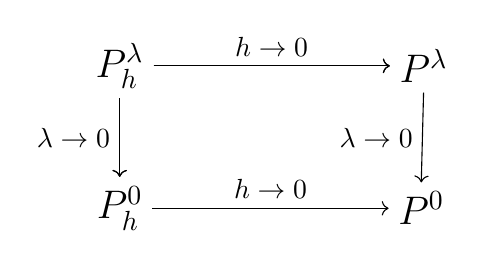
\begin{tikzpicture}
    \node (nw) {\Large $P^\lambda_h$};
    \node (ne) [right=3cm of nw]{\Large $P^\lambda$};
    \node (sw) [below=of nw]{\Large $P^0_h$};
    \node (se) [right=3cm of sw]{\Large $P^0$};
    \draw[->] (nw.east)  -- node [above,midway] {$h\rightarrow0$} (ne.west) ;
    \draw[->] (nw.east)  --  (ne.west) ;
    \draw[->] (nw.south) -- node [left,midway] {$\lambda\rightarrow0$} (sw.north);
    \draw[->] (nw.south) -- node {} (sw.north);
    \draw[->] (sw.east)  -- node [above,midway] {$h\rightarrow0$}(se.west);
    \draw[->] (ne.south) -- node [left,midway] {$\lambda\rightarrow0$} (se.north);
    \end{tikzpicture}
    \caption{Commuting diagram of AP schemes}
    \label{fig:commutative_diagram_ap}
\end{figure}

The content of this paper is organized as follows. In Section 2, we first give full details on the underlying equations of the Maxwell-Euler system and its rescaling procedure. Afterwards we introduce the ECE-type boundary conditions for our problem. A reformulation of Maxwell's equations in the insulating region is then presented. Section 3 is devoted to the discretization. \todo{outline}  

\begin{figure}
    \centering
    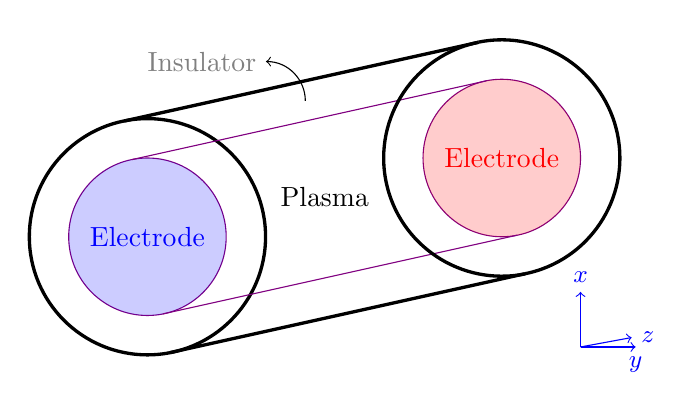
\begin{tikzpicture}
    \coordinate (O1) at (0,0);
    \draw[violet] (O1) circle (1) node[blue] {Electrode};
    \fill[blue, opacity=0.2] (O1) circle (1);
    \draw[very thick] (O1) circle (1.5);
    \coordinate (O2) at (4.5,1);
    \draw[violet] (O2) circle (1);
    \node at (O2) {\textcolor{red}{Electrode}};
    \node at (barycentric cs:O1=1,O2=1) {Plasma}; 
    \fill[red, opacity=0.2] (O2) circle (1);
    \coordinate (S1) at ([shift={(-0.196,0.98)}]O1);
    \coordinate (S2) at ([shift={(-0.196,0.98)}]O2);
    \coordinate (P1) at ([shift={(0.196,-0.98)}]O1);
    \coordinate (P2) at ([shift={(0.196,-0.98)}]O2);
    \draw[violet] (S1) -- (S2);
    \draw[violet] (P1) -- (P2);
    \coordinate (SS1) at ([shift={({-0.196*1.5},{0.98*1.5})}]O1);
    \coordinate (SS2) at ([shift={({-0.196*1.5},{0.98*1.5})}]O2);
    \coordinate (PP1) at ([shift={({0.196*1.5},{-0.98*1.5})}]O1);
    \coordinate (PP2) at ([shift={({0.196*1.5},{-0.98*1.5})}]O2);
    \draw[very thick] (SS1) -- (SS2);
    \draw[very thick] (PP1) -- (PP2); 
    \draw[black, very thick] (SS2) arc (101.31:180+101.31:1.5);
    \draw[very thick] (PP2) arc (101.31-180:101.31:1.5);
    \draw[-to] (barycentric cs:SS1=1,SS2=1,S1=1,S2=1) to[out=90,in=0] ([shift={(-0.5,0.5)}]barycentric cs:SS1=1,SS2=1,S1=1,S2=1) node[left, gray] {Insulator};
    \begin{scope}[shift={(5.5,-1.4)}]
    \draw[blue, -to] (0,0) -- (0.65,0.12) node[right]{\small $z$};
    \draw[blue, -to] (0,0) -- (0,0.7) node[above]{\small $x$};
    \draw[blue, -to] (0,0) -- (0.7,0) node[below]{\small $y$};
    \end{scope}
    \end{tikzpicture}
\caption{The domain geometry}
\label{fig:domain_geometry}
\end{figure}



\section{Plasma model}
\begin{comment}
Under moderate assumptions, plasmas, which are gases composed of charged particles (and possibly neutral particles), can be treated as fluid and described by hydrodynamic equations. Maxwell's equations are involved to describe their induction of and interaction with electromagnetic fields. 

After rescalling all the variables with respect to the prescribed reference units, the Debye length $\lambda_D$, characterizing the charge screening ability of the plasma, would pop up and its zero limit, which is what we called \emph{quasi-neutral limit}, is of great interest, since the limit model largely simplifies the system and in many cases the accuracy of the assumption is satisfactory enough. 

In this section, the multi-species Maxwell-Euler equations with collision term is introduced first, followed by detailed rescalling procedure. The quasi-neutral model will be make clear by letting the rescaled Debye length $\lambda$ go to zero. Afterwards, a set of boundary conditions are presented and its validity to both non-limit and limit model is discussed. Finally, we would like to present a reformulation of the system which would be crucial to the stability of the numerical scheme.
\end{comment}

\begin{comment}
In this work, we discuss and implement the so-called \emph{Euler-Maxwell} system with a focus on its limiting behavior of quasi-neutrality, namely when the \emph{Debye length} goes to zero. The dimensionless form of the Euler-Maxwell equations is parameterized by the rescaled Debye length $\lambda$ whose vanishing limit alters the mathematical nature of the equations. To be more concrete, the non-limit model ($\lambda = \mathcal{O}(1)$) is hyperbolic where information spreads with a finite speed whereas the limit model ($\lambda \rightarrow 0$) becomes elliptic, and any changes immediately influence the whole domain. In other words, the perturbation of $\lambda$ in the Maxwell-Euler system poses a singular perturbation problem. Such switching makes it difficult to handle both models in a single implementation framework, which, however, is desired in many cases where both models coexist in the computational domain. Now comes the concept of \emph{asymptotic-preserving}(AP) scheme. We turn to the celebrated commuting diagram Fig. \ref{fig:commuting_diagram_ap} for illustration.\todo{add illustration of AP schemes}.

The other emphasis of this work is the development of a 3D discretization framework for the Maxwell-Euler system. The key ingredient is the combination of the Finite Volume Method (FVM) for the Euler equations and the Finite Integration Technique (FIT) for Maxwell's equations. The latter one is usually treated as a generalization to Yee's scheme \citep{yee_1966} or FDTD. The advantage of the FVM-FIT framework lie in the \emph{discrete exterior calculus} (DEC) nature of FIT and straightforward coupling of both systems through the primal-dual mesh pair. These would be made clear in the corresponding sections. 

\todo{add previous work on AP schemes, FIT, plasma simulation}.

The content of this paper is organized as follows. In Section 2 we introduce the full Maxwell-Euler model for plasmas, followed by the rescaling procedure which is crucial to define the rescaled Debye length $\lambda$ and to identify its limiting behavior. In the meantime, it is essential to discuss what boundary conditions are appropriate for this singular perturbation problem. Section 3 is then dedicated to a brief introduction about \cite{degond_2012} based on which our work is extended. In Section 4, we first discuss our FVM-FIT framework in details, especially how the unknowns are assigned on the staggered meshes and the boundary treatment in 3D case. Afterwards, the full discretization scheme is presented. Special care shall be taken to the treatment of boundary conditions and insulator part of the domain as $\lambda \rightarrow 0$, which is crucial to make the scheme AP. A numerical experiment for a 3D cylindrical domain is presented in Section 5 where we want to demonstrate the capability of our scheme in dealing with both non-neutral and quasi-neutral regimes of plasmas.    

\begin{figure}
    \centering
    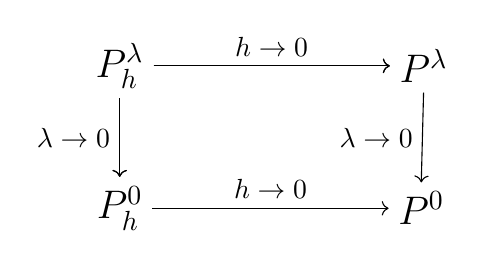
\begin{tikzpicture}
    \node (nw) {\Large $P^\lambda_h$};
    \node (ne) [right=3cm of nw]{\Large $P^\lambda$};
    \node (sw) [below=of nw]{\Large $P^0_h$};
    \node (se) [right=3cm of sw]{\Large $P^0$};
    \draw[->] (nw.east)  -- node [above,midway] {$h\rightarrow0$} (ne.west) ;
    \draw[->] (nw.east)  --  (ne.west) ;
    \draw[->] (nw.south) -- node [left,midway] {$\lambda\rightarrow0$} (sw.north);
    \draw[->] (nw.south) -- node {} (sw.north);
    \draw[->] (sw.east)  -- node [above,midway] {$h\rightarrow0$}(se.west);
    \draw[->] (ne.south) -- node [left,midway] {$\lambda\rightarrow0$} (se.north);
    \end{tikzpicture}
    \caption{Commuting diagram of AP schemes}
    \label{fig:commuting_diagram_ap}
\end{figure}
\end{comment}

\subsection{The Maxwell-Euler System}
Under moderate assumptions, plasmas, which are gases composed of charged particles (and possibly neutral particles), can be treated as fluids governed by hydrodynamic equations. Maxwell's equations take charge of their interaction with electromagnetic fields. For more details on the fluid model of plasma, see \cite{chen2016, remi_2014}.

The Maxwell's equations in SI units read
\begin{subequations}
\begin{align}
    \partial_t \mathbf{B} + \nabla \times \mathbf{E} &= 0, \label{equ:maxwell_faraday} \\ 
    \partial_t \mathbf{D} - \nabla \times \mathbf{H} &= -\mathbf{J}, \label{equ:maxwell_ampere} \\
    \nabla \cdot \mathbf{B} &= 0,  \label{equ:maxwell_gauss_B}\\
    \nabla \cdot \mathbf{D} &= \rho, \label{equ:maxwell_gauss_D}
\end{align}
\end{subequations}
where the involved quantities are magnetic flux density $\mathbf{B}$, electric field intensity $\mathbf{E}$, electric induction $\mathbf{D}$, magnetic field intensity $\mathbf{H}$, electric current density $\mathbf{J}$ and electric charge density $\rho$. These equations are known as Faraday's law (\ref{equ:maxwell_faraday}), Amp\`{e}re's law (\ref{equ:maxwell_ampere}), Gauss's law for magnetism (\ref{equ:maxwell_gauss_B}) and Gauss's law for electric field (\ref{equ:maxwell_gauss_D}). For simplicity, we only consider isotropic and homogeneous media in vacuum. We consider the linear constitutive relations 
\begin{equation} \label{equ:material_law}
    \mathbf{D} = \varepsilon_0 \mathbf{E}, \ \ \ \mathbf{B} = \mu_0\mathbf{H}, 
\end{equation}
where $\varepsilon_0$ and $\mu_0$ are the vacuum permittivity and permeability of the medium. By definition of the electric current density $\mathbf{J}$ and electric charge density $\rho$, they are supposed to satisfy the continuity equation
\begin{equation} \label{equ:charge_continuity}
    \partial_t\rho + \nabla \cdot \mathbf{J} = 0.
\end{equation}
Besides, on taking the divergence of equations (\ref{equ:maxwell_faraday}) and (\ref{equ:maxwell_ampere}) together with the relation (\ref{equ:charge_continuity}), it is possible to verify that Gauss's laws (\ref{equ:maxwell_gauss_B}) (\ref{equ:maxwell_gauss_D}) are consequences of (\ref{equ:maxwell_faraday}) and (\ref{equ:maxwell_ampere}) provided that (\ref{equ:maxwell_gauss_B}) (\ref{equ:maxwell_gauss_D}) are satisfied at the initial time. In other words, Gauss's laws (\ref{equ:maxwell_gauss_B}) (\ref{equ:maxwell_gauss_D}) can be thought of as initial conditions. 

Each species in plasmas are treated as a compressible flow and assocated to one set of Euler equations that includes electromagnetic forces as well as other processes, e.g. collisions and recombination. The generic expressions are
\begin{align} \label{equ:euler_}
    \partial_t
    \begin{bmatrix}
    n_* \\
    m_*n_* \mathbf{u}_* \\
    m_*n_* e_*
    \end{bmatrix}
    + \nabla \cdot
    \begin{bmatrix}
    n_* \mathbf{u}_* \\
    m_*n_* \mathbf{u}_* \otimes \mathbf{u}_* + p_*\mathbb{I} \\
    m_*n_* h_* \mathbf{u}_*
    \end{bmatrix}
    =
    \begin{bmatrix}
    0 \\
    q_*n_*(\mathbf{E} + \mathbf{u}_* \times \mathbf{B}) \\
    \mathbf{J}_* \cdot \mathbf{E}
    \end{bmatrix}
    +
    \begin{bmatrix}
    \Gamma_* \\
    \mathbf{R}_* \\
    Q_*
    \end{bmatrix}.
\end{align}
The subscript $*$ represents the indices for different species, and by convention we assign $* = e$ to electrons, $* = i$ to ions, and $* = n$ to neutral atoms. The involved fluid quantities are: number density $n_*$, particle mass $m_*$,  charge number $q_*$, velocity $\mathbf{u}_*$, pressure $p_*$, specific total energy $e_* := \frac{1}{2}|\mathbf{u}_*|^2 + \frac{p_*}{m_*n_*(\gamma - 1)}$, specific total enthalpy $h_* := e_* + \frac{p_*}{m_*n_*}$ and current density $\mathbf{J}_* := q_*n_*\mathbf{u}_*$. All the species are assumed ideal gases with heat capacity ratio $\gamma=5/3$ for monatomic gases. The left-hand side of the equations describes the convection of plasma fluids. The first term at the right-hand side denotes Lorentz force in the momentum equation and Joule heating in the energy equation. $\Gamma_*, \mathbf{R}_*, Q_*$ are generic terms due to effects of inter-species collision, ionization, recombination, etc. 

For the sake of simplicity for presentation, we only consider ion-electron collision in this work, but extension to more species is straightforward. Under moderate assumptions, such collisions can be well modelled by frictions, and we simply present the expressions without derivation (see \citep[][sec. 5.6.2]{chen2016}):
\begin{equation} \label{equ:collision}
    \mathbf{R}_{e}^{\text{coll}} = \frac{\pi Ze^4m_e^{1/2}}{(4\pi\varepsilon_0)^2(k_BT_e)^{3/2}}\text{ln}\Lambda n_en_i(\mathbf{u}_i - \mathbf{u}_e) = - \mathbf{R}_{i}^{\text{coll}},  
\end{equation}
which models the collision force that is applied on the electrons. ln$\Lambda$ is called the \emph{Coulomb logarithm}, which typically takes a numerical value of order 10–20 . Because of the conservation of momentum, the collision term for ions $\mathbf{R}_{i}^{\text{coll}}$ is nothing but the negation of $\mathbf{R}_{e}^{\text{coll}}$. In this work, the other effects, e.g. ionization and recombination, are not considered. For full details about the modeling of these physical processes, readers are referred to \cite{fuchs_2021}.  


Combination of the two sets of equations (\ref{equ:maxwell_faraday}) to (\ref{equ:maxwell_gauss_D}) and (\ref{equ:euler_}) leads to the governing equations for a multi-species plasma model. The coupling of the two subsystems is due to the following relations that connect the fluid and electromagnetic quantities
\begin{equation} \label{equ:maxwell_euler_coupling}
    \rho = \sum_* q_*n_*, \ \ \  \mathbf{J} = \sum_* q_*n_*\mathbf{u}_*. 
\end{equation}

\subsection{Rescaling} \label{sec:rescaling}
In the rescaling, the variables in the equations are taken as the ratio of their original quantities and reference units, which transforms the system into dimensionless form. In this part, the rescaling procedure mostly follows that of \cite{degond_2017}.

First, reference units for each quantity, e.g. the characteristic length and time scale, are prescribed. We define $\overline{x}$ and $\overline{t}$ as space and time scale of interest, by which the reference velocity $\overline{v}$ is defined as $\overline{x}/\overline{t}$. The typical magnitudes of electromagnetic fields are $\overline{E}$ and $\overline{B}$. The typical magnitudes of fluid quantities are denoted by $\overline{u}$ for plasma drift velocity, $\overline{n}$ for plasma number density, $\overline{T}$ for plasma temperature. On top of that, the typical pressure is set $\overline{n}k_B\overline{T}$ with $k_B$ being the Boltzmann constant; the typical value for the specific total energy and enthalpy is set $\overline{u}^2$. Together with the physical parameters, namely, permittivity $\varepsilon_0$, permeability $\mu_0$, light speed $c^2 = (\varepsilon_0\mu_0)^{-1}$, Boltzmann constant $k_B$, the elementary charge $e$, and ion mass $m_i$, the following dimensionless parameters are induced,
\begin{align*} 
    \xi &:= \frac{\overline{v}}{c} \text{ the velocity of interest \emph{w.r.t.}\footnotemark[1] the light speed}, &\\
    \zeta &:= \frac{\overline{u}}{\overline{v}} \text{ the plasma velocity \emph{w.r.t.} the speed of interest}, &\\
    M &:= \frac{\overline{u}}{v_{th,i}} \text{ the plasma drift velocity \emph{w.r.t.} the thermal speed of ions, where } v_{th,i} := \left(\frac{k_B \overline{T}}{m_i}\right)^{1/2}, &\\
    \eta &:= \frac{e\overline{E}\overline{x}}{m_i\overline{u}^2} \text{ the electric energy \emph{w.r.t.} the kinetic energy of ions}, &\\
    \beta &:= \frac{\overline{v}\overline{B}}{\overline{E}} \text{ the induced electric field \emph{w.r.t.} the total electric field}, &\\
    \lambda &:= \frac{\lambda_D}{\overline{x}} \text{ the dimensionless Debye length, where }\lambda_D := \left(\frac{\varepsilon_0k_B\overline{T}}{e^2\overline{n}}\right)^{1/2}, &\\
    \varepsilon_*^2 &:= \frac{m_*}{m_i} \text{ the species mass \emph{w.r.t.} the ion mass},\ \  * \in \{i,e,n,\cdots\}, &\\
    g &:= \frac{1}{\overline{n}\lambda_D^3} \text{ the plasma parameter\footnotemark[2]}.&
\end{align*}
\footnotetext[1]{Abbreviation of \emph{with respect to}.}
\footnotetext[2]{It is basically the reciprocal of the number of particles per Debye sphere, see \cite[][sec. 1.1]{gibbon2020}. Classical plasma theory assumes $g \ll 1$.} 

By abuse of notation, the dimensionless quantities have the same symbol with their original ones without incurring any ambiguity. For the sake of simplicity, we only consider the collision terms, namely $\Gamma_* = 0, \mathbf{R}_* = \mathbf{R}_*^\text{coll}, Q_* = Q_*^\text{coll}$ in (\ref{equ:euler_}), while neglecting other effects. The rescaled Euler-Maxwell system reads
\begin{subequations}
\begin{align}
    \beta \partial_t \mathbf{B} + \nabla \times \mathbf{E} &= 0, \label{equ:maxwell_faraday_rescalling} \\ 
    \lambda^2 \partial_t \mathbf{D} - \frac{\beta \lambda^2}{\xi^2}\nabla \times \mathbf{H} &= - \frac{\zeta}{\eta M^2}\mathbf{J}, \label{equ:maxwell_ampere_rescalling} \\
    \nabla \cdot \mathbf{B} &= 0,  \label{equ:maxwell_gauss_B_rescalling}\\
    \lambda^2 \eta M^2 \nabla \cdot \mathbf{D} &= \rho, \label{equ:maxwell_gauss_D_rescalling} \\
    \partial_t
    \begin{bmatrix}
    n_* \\
    n_* \mathbf{u}_* \\
    n_* e_*
    \end{bmatrix}
    + \nabla \cdot
    \begin{bmatrix}
    \zeta n_* \mathbf{u}_* \\
    \zeta n_* \mathbf{u}_* \otimes \mathbf{u}_* + \zeta M^{-2} \varepsilon_*^{-2} p_*\mathbb{I} \\
    \zeta n_* h_* \mathbf{u}_*
    \end{bmatrix}
    &=
    \begin{bmatrix}
    0 \\
    \eta \zeta \varepsilon_*^{-2} q_* n_*\mathbf{E} + \eta \zeta^2 \beta \varepsilon_*^{-2} q_* n_* \mathbf{u}_* \times \mathbf{B} \\
    \zeta \eta \varepsilon_*^{-2} \mathbf{J}_* \cdot \mathbf{E}
    \end{bmatrix} +
    \begin{bmatrix}
    0 \\
    \varepsilon_*^{-2}\mathbf{R}_*^{\text{coll}} \\
    \varepsilon_*^{-2}Q_*^{\text{coll}} \\
    \end{bmatrix}, \label{equ:euler_rescalling}
\end{align}
\end{subequations}
where the equation of state becomes $e_* = \frac{1}{2}|\mathbf{u_*}|^2 + M^{-2}\frac{p_*}{\epsilon^2_* n_* (\gamma - 1)}$ and $h_* = e_* + M^{-2}\frac{p_*}{\epsilon^2_* n_*}$. For a fully-ionized gas, we have the original expression of $\mathbf{R}_*^{\text{coll}}$ in (\ref{equ:collision}), and its rescaled expression becomes
\begin{equation*}
    \mathbf{R}_i^{\text{coll}} = \frac{Z\text{ln}\Lambda}{16\pi}g\lambda^{-1}M^{-1}\varepsilon_en_en_i(\mathbf{u}_i - \mathbf{u}_e). 
\end{equation*}

Following the assumption in \cite{degond_2017}, the reference speed $\overline{v}$ is of the same scale with the plasma speed $\overline{u}$ and the thermal speed $v_{th,i}$ whereas it is much smaller than the light speed $c$. To study the quasi-neutral regime, the dimensionless Debye length $\lambda$ is an asymptotic parameter ranging in $[0,1]$. It is assumed that $\alpha$ has the same magnitude as $\lambda$, and $\eta$ and $\beta$ are of order one. 

Special treatment is needed for the collision term. One would notice the inverse proportionality to $\lambda$, which would introduce a singular perturbation to the Euler system as $\lambda \rightarrow 0$. However, the validity of such a collision model is doubtful when $\lambda \rightarrow 0$. From the physical viewpoint, the shielding effect characterized by Debye length $\lambda$ makes the impact parameter no larger than $\lambda$. The $\lambda \rightarrow 0$ limit implies that the collisions happen in the atomic length scale, in which quantum-mechanical effects must be taken into effect \citep{frank_1972}. Therefore, for the sake of simplicity, we eliminate the perturbation parameter in the friction term by assuming $g \sim \lambda$ and keep the prefactor of collision term constant $\alpha^{\text{coll}}$ throughout the simulation.

\begin{remark}
    It is also of research interest when there is an asymptotic parameter at the denominator of the friction term. Such problem is called relaxation limit, see \cite{peng_2011, wasiolek_2016, Li_2021, Chen_2000}.
\end{remark}

In summary, we make the following choices
\begin{align*}
    \xi \sim g \sim \lambda \in [0,1], \ \ \ \zeta \sim M \sim \eta \sim \beta \sim \mathcal{O}(1).
\end{align*}


Under such assumptions on these dimensionless parameters, the rescaled Euler-Maxwell system is simplified into a parametric system with the dimensionless Debye length $\lambda$ being the asymptotic parameter
\begin{subequations}
\begin{align}
    \partial_t \mathbf{B} + \nabla \times \mathbf{E} &= 0, \label{equ:maxwell_faraday_rescaled} \\ 
    \lambda^2 \partial_t \mathbf{D} - \nabla \times \mathbf{H} &= - \mathbf{J}, \label{equ:maxwell_ampere_rescaled} \\
    \nabla \cdot \mathbf{B} &= 0,  \label{equ:maxwell_gauss_B_rescaled}\\
    \lambda^2 \nabla \cdot \mathbf{D} &= \rho, \label{equ:maxwell_gauss_D_rescaled} \\
    \partial_t
    \begin{bmatrix}
    n_* \\
    n_* \mathbf{u}_* \\
    n_* e_*
    \end{bmatrix}
    + \nabla \cdot
    \begin{bmatrix}
    n_* \mathbf{u}_* \\
    n_* \mathbf{u}_* \otimes \mathbf{u}_* + \varepsilon_*^{-2} p_*\mathbb{I} \\
    n_* h_* \mathbf{u}_*
    \end{bmatrix}
    &=
    \begin{bmatrix}
    0 \\
    \varepsilon_*^{-2} q_* n_* (\mathbf{E} + \mathbf{u}_* \times \mathbf{B}) \\
    \varepsilon_*^{-2} \mathbf{J}_* \cdot \mathbf{E}
    \end{bmatrix}+
    \begin{bmatrix}
    0 \\
    \varepsilon_*^{-2}\mathbf{R}_*^{\text{coll}} \\
    \varepsilon_*^{-2}Q_*^{\text{coll}} 
    \end{bmatrix}, \label{equ:euler_rescaled}
\end{align}
\end{subequations}
with the equation of state $e_* = \frac{1}{2}|\mathbf{u_*}|^2 + \frac{p_*}{\varepsilon^2_* n_* (\gamma - 1)}$ and $h_* = e_* + \frac{p_*}{\varepsilon^2_* n_*}$. For a fully-ionized gas with only ions and electrons, 
\begin{equation} \label{equ:collision_rescaled} 
    \mathbf{R}_i^{\text{coll}} = \alpha^{\text{coll}}n_en_i(\mathbf{u}_i - \mathbf{u}_e) = - \mathbf{R}_e^{\text{coll}},
\end{equation}
and consequently, the rescaled friction heat for ions and electrons takes the expression
\begin{align*} 
    Q_i^{\text{coll}} &= \alpha^{\text{coll}}n_en_i \mathbf{u}_i (\mathbf{u}_i - \mathbf{u}_e), \\
    Q_e^{\text{coll}} &= \alpha^{\text{coll}}n_en_i \mathbf{u}_e (\mathbf{u}_e - \mathbf{u}_i).
\end{align*}

We end up getting the rescaled Maxwell-Euler system parameterized by $\lambda$. The rescaling enables us to identify the magnitude of each term in the equations, which is revealed by the prefactor polynomial of $\lambda$.  

\subsection{Quasi-neutral Limit} \label{sec:quasi-neutral_limit}
The Debye length $\lambda_D$ (see its definition at the preceding section) is an characteristic length over which local concentrations of charge are shielded out. For the underlying physics, see \cite[Sec. 1.4]{chen2016}. In many situations, it has a rather low value compared to the interested length scale: the typical $\lambda_D$ for gas discharge and Tokamak is $10^{-4}$ m; for interstellar medium, the magnitude is about $1$ m \cite[ch. 20]{Blandford_2013}. That justifies the quasi-neutrality assumption that the plasma is locally neutral, namely $\rho = \sum_* q_*n_* = 0$. The limit model is obtained by formally taking the rescaled Debye length $\lambda$ to zero:
\vspace{-\baselineskip}
\begin{center}
    \begin{minipage}{0.3\textwidth}
\begin{subequations}
\begin{align*}
    \partial_t \mathbf{B} + \nabla \times \mathbf{E} &= 0,\\ 
    \lambda^2 \partial_t \mathbf{D} - \nabla \times \mathbf{H} &= - \mathbf{J}, \\
    \nabla \cdot \mathbf{B} &= 0, \\
    \lambda^2 \nabla \cdot \mathbf{D} &= \rho.
\end{align*}
\end{subequations}

\end{minipage}
$\xrightarrow[]{\lambda \rightarrow 0}$
\begin{minipage}{0.3\textwidth}
\begin{subequations}
\begin{align}
    \partial_t \mathbf{B} + \nabla \times \mathbf{E} &= 0, \label{equ:maxwell_faraday_limit} \\ 
    - \nabla \times \mathbf{H} &= - \mathbf{J}, \label{equ:maxwell_ampere_limit} \\
    \nabla \cdot \mathbf{B} &= 0,  \label{equ:maxwell_gauss_B_limit}\\
     0 &= \rho. \label{equ:maxwell_gauss_D_limit}
\end{align}
\end{subequations}
\end{minipage}
\end{center}
The quasi-neutral condition (\ref{equ:maxwell_gauss_D_limit}) is the consequence of taking $\lambda = 0$ in Gauss's law for electric field (\ref{equ:maxwell_gauss_D_rescaled}). Like the non-neutral case, Gauss's laws (\ref{equ:maxwell_gauss_B_limit}) (\ref{equ:maxwell_gauss_D_limit}) are the consequence of (\ref{equ:maxwell_faraday_limit}) (\ref{equ:maxwell_ampere_limit}) provided (\ref{equ:maxwell_gauss_B_limit}) (\ref{equ:maxwell_gauss_D_limit}) are satisfied at initial time. 


This limit poses a \emph{singular perturbation problem} in the sense that vanishing $\lambda$ changes the character of the PDE system. To be more specific, in the non-limit model the $\mathbf{E}$-field evolves with time whereas in the quasi-neutral model it responds instantaneously to other quantities according to the constraint (\ref{equ:maxwell_ampere_limit}). To make it clear, we replace the equation (\ref{equ:maxwell_ampere_rescaled}) by the sum of the curl of (\ref{equ:maxwell_faraday_rescaled}) and the time-derivative of (\ref{equ:maxwell_ampere_rescaled}). Meanwhile exploiting the momentum equation in (\ref{equ:euler_rescaled}) to express $\partial_t\mathbf{J}$, we end up getting the equation that the $\mathbf{E}$-field satisfies
\begin{align}
    \lambda^2\partial_t^2 \mathbf{E} + \nabla \times \nabla \times \mathbf{E} &= - a\mathbf{E} - \mathbf{b}, \label{equ:E}
\end{align}
where
\begin{equation*}
    a = \sum_*\varepsilon_*^{-2}q_*^2n_*, \ \ \ \mathbf{b} = \sum_* \epsilon_*^{-2}q_*^2n_*\mathbf{u}_*\times\mathbf{B} - q_*\nabla\cdot(n_* \mathbf{u}_* \otimes \mathbf{u}_* + \varepsilon_*^{-2}p_*\mathbb{I}).
\end{equation*}
 The equation (\ref{equ:E}) implies the shift from the hyperbolic nature to the elliptic nature of the $\mathbf{E}$-field as $\lambda\rightarrow0$. 

\begin{remark}
    The preceeding formal limit argument is rather heuristic. Deep mathematical tools from perturbation theory is needed to rigorously prove the convergence of the limiting sequence. This topic is beyond the scope of this paper and thus omitted. Readers are referred to \cite[ch. 2]{remi_2014} \cite{Peng_2008} for the quasi-neutral limit of the Maxwell-Euler system, and \cite{mark_1995, Eckhaus_1980} for the general theory.
\end{remark} 

\subsection{Boundary Conditions} \label{sec:BC}

We consider a simply connected domain $\Omega$ that is decomposed into two sub-domains $\Omega_P$ and $\Omega_I$ representing plasma domain and insulating domain respectively. We use the notation $\Gamma_C := \partial\Omega \cap \partial\Omega_P$, denoting the contact boundary, and $\Gamma_I := \partial\Omega \cap \partial\Omega_I$ for the insulating boundary which an artificial cut-off boundary. The interface between the two domains is denoted by $\Gamma_W = \partial\Gamma_I \cap \partial\Gamma_P$. A geometric arrangement corresponding to his setting is visualized in Fig. \ref{fig:domain_sketch}. 

The plasma fills $\Omega_P$ where the Euler system is defined and the boundary of plasmas lies on $\partial\Omega_P$. We consider the physical scenario where plasmas are confined with the solid insulator. Therefore, the interface $\Gamma_W$ is treated as reflective walls where fluid particles are bounced back while keeping the tangential velocity and energy unchanged. The contact boundary $\Gamma_C$ is where the plasma and energy flow across, modelled by open boundaries in the sense that they are free to flow through, namely, ions and electrons are emitted and absorbed by the electron. 

\begin{remark}
    The treatment of electrodes as open boundary is a rather simplified approach. For more realistic electrode modelling, see \cite{godyak_1990, parker_1993}.
\end{remark}

The Maxwell system is defined on the whole domain $\Omega$. External voltages are enforced on the contact boundary $\Gamma_C$ to model electrodes. More specifically, $\Gamma_C$ is composed of two disjoint connecting components $\Gamma_C^\pm$. Constant potentials are enforced on each component in the sense that $\Phi|_{\Gamma_C^\pm} = \Phi_\pm$. The insulating boundary blocks the energy interchange and therefore only admits zero electric and magnetic flux, in the sense that $\text{curl}\mathbf{E}\cdot \mathbf{n} = 0$ and $\text{curl}\mathbf{H}\cdot \mathbf{n} = 0$ where $\mathbf{n}$ is the outer normal vector. \todo{A few works on ECE BC?} 
\begin{figure}
\begin{minipage}{0.45\textwidth}
    \resizebox{\textwidth}{!}{
    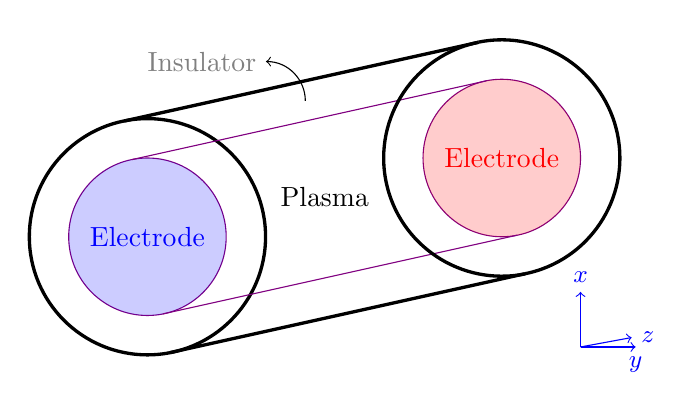
\begin{tikzpicture}
    \coordinate (O1) at (0,0);
    \draw[violet] (O1) circle (1) node[blue] {Electrode};
    \fill[blue, opacity=0.2] (O1) circle (1);
    \draw[very thick] (O1) circle (1.5);
    \coordinate (O2) at (4.5,1);
    \draw[violet] (O2) circle (1);
    \node at (O2) {\textcolor{red}{Electrode}};
    \node at (barycentric cs:O1=1,O2=1) {Plasma}; 
    \fill[red, opacity=0.2] (O2) circle (1);
    \coordinate (S1) at ([shift={(-0.196,0.98)}]O1);
    \coordinate (S2) at ([shift={(-0.196,0.98)}]O2);
    \coordinate (P1) at ([shift={(0.196,-0.98)}]O1);
    \coordinate (P2) at ([shift={(0.196,-0.98)}]O2);
    \draw[violet] (S1) -- (S2);
    \draw[violet] (P1) -- (P2);
    \coordinate (SS1) at ([shift={({-0.196*1.5},{0.98*1.5})}]O1);
    \coordinate (SS2) at ([shift={({-0.196*1.5},{0.98*1.5})}]O2);
    \coordinate (PP1) at ([shift={({0.196*1.5},{-0.98*1.5})}]O1);
    \coordinate (PP2) at ([shift={({0.196*1.5},{-0.98*1.5})}]O2);
    \draw[very thick] (SS1) -- (SS2);
    \draw[very thick] (PP1) -- (PP2); 
    \draw[black, very thick] (SS2) arc (101.31:180+101.31:1.5);
    \draw[very thick] (PP2) arc (101.31-180:101.31:1.5);
    \draw[-to] (barycentric cs:SS1=1,SS2=1,S1=1,S2=1) to[out=90,in=0] ([shift={(-0.5,0.5)}]barycentric cs:SS1=1,SS2=1,S1=1,S2=1) node[left, gray] {Insulator};
    \begin{scope}[shift={(5.5,-1.4)}]
    \draw[blue, -to] (0,0) -- (0.65,0.12) node[right]{\small $z$};
    \draw[blue, -to] (0,0) -- (0,0.7) node[above]{\small $x$};
    \draw[blue, -to] (0,0) -- (0.7,0) node[below]{\small $y$};
    \end{scope}
    \end{tikzpicture}}
\end{minipage}
\begin{minipage}{0.49\textwidth}
    \resizebox{1.1\textwidth}{!}{ 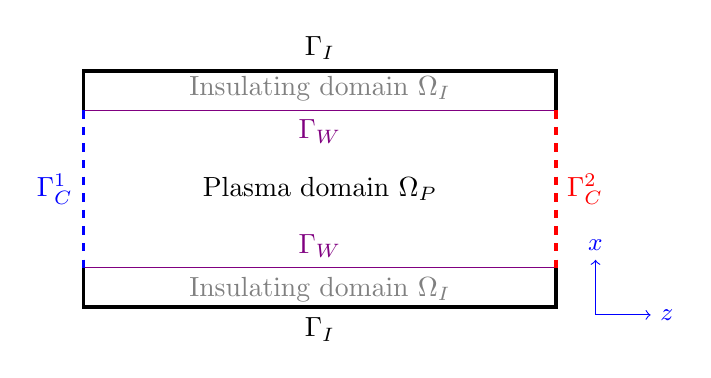
\begin{tikzpicture}
        \coordinate (A1) at (0,1.5);
        \coordinate (A2) at (0,1);
        \coordinate (A3) at (0,-1);
        \coordinate (A4) at (0,-1.5);
        \coordinate (B1) at (6,1.5);
        \coordinate (B2) at (6,1);
        \coordinate (B3) at (6,-1);
        \coordinate (B4) at (6,-1.5);
        \draw[violet] (A2) -- node[above]{\color{gray}Insulating domain $\Omega_I$} node[black, below]{\textcolor{violet}{$\Gamma_W$}} (B2);
        \draw[violet] (A3) -- node[below]{\color{gray}Insulating domain $\Omega_I$} node[black, above]{\textcolor{violet}{$\Gamma_W$}} (B3);
        \draw[very thick] (A2) -- (A1) -- node[above]{$\Gamma_I$}  (B1) -- (B2);
        \draw[very thick] (A3) -- (A4) -- node[below]{$\Gamma_I$} (B4) -- (B3);
        \draw[very thick, dashed, blue] (A2) -- node[left] {$\Gamma_C^1$} (A3);
        \draw[very thick, dashed, red]  (B2) -- node[right] {$\Gamma_C^2$}  (B3);
        \node at (3,0) {Plasma domain $\Omega_P$};
        \begin{scope}[shift={(6.5,-1.6)}]
        \draw[blue, -to] (0,0) -- (0,0.7) node[above]{\small $x$};
        \draw[blue, -to] (0,0) -- (0.7,0) node[right]{\small $z$};
        \end{scope}
    \end{tikzpicture}}
\end{minipage}
\caption{Sketch of the domain. The right figure shows the cross section on the $x$-$z$ plane.}
\label{fig:domain_sketch}
\end{figure}


    To summarize the boundary conditions for both systems:
    
\vspace{10pt}
\begin{minipage}[t]{0.49\textwidth}
    \textbf{For the Euler equations:}
    \begin{align*}
    \mathbf{u_*}\cdot \mathbf{n} &= 0 \ \ \text{on} \ \ \Gamma_W, \\
    \text{grad}n_* \cdot \mathbf{n} &= 0 \ \ \text{on} \ \ \Gamma_W. \\
    \text{grad}e_* \cdot \mathbf{n} &= 0 \ \ \text{on} \ \ \Gamma_W. \\
    \text{grad}\mathbf{U_*} \cdot \mathbf{n} &= \mathbf{0} \ \ \text{on} \ \ \Gamma_C.
\end{align*}
\end{minipage}
\begin{minipage}[t]{0.49\textwidth}
    \textbf{For Maxwell's equations:}
    \begin{align*}
    \Phi = \Phi^\pm(t)\ \ &\text{on} \ \ \Gamma_C^\pm, \\
    \text{curl} \mathbf{E} \cdot \mathbf{n} = 0\ \ &\text{on} \ \  \Gamma_I,  \\
    \text{curl} \mathbf{H} \cdot \mathbf{n} = 0\ \ &\text{on} \ \  \Gamma_I.\
    \end{align*}
\end{minipage}

\vspace{10pt}

\begin{remark}
    A small remark goes to the validity of assignment of electric potentials on $\Gamma_c^\pm$. Since the surface curl $\text{\emph{curl}}_\gamma\mathbf{E} = \text{\emph{curl}} \mathbf{E} \cdot \mathbf{n} = 0$, there exists a surface potential $\varphi$ such that the surface gradient $\nabla_\Gamma \varphi = \gamma_\tau \mathbf{E}$ where $\gamma_\tau $ is the tangential trace operator. However, for a geometric setting with non-trivial geometry, one needs to consider co-homology vector fields \cite{Hiptmair_2021}.
\end{remark}



\subsection{Reformulation} \label{sec:reform_continuous}
In the insulating domain $\Omega_I$ (see Fig. \ref{fig:sketch_domain}), the Euler system is not defined there due to the absence of plasmas. Consequently, the Maxwell system in $\Omega_I$ is described by
\begin{subequations}
\begin{align}
    \partial_t \mathbf{B} + \nabla \times \mathbf{E} &= 0, \label{equ:faraday_ins}\\ 
    \lambda^2 \partial_t \mathbf{D} - \nabla \times \mathbf{H} &= 0,  \label{equ:ampere_ins}\\
    \nabla \cdot \mathbf{B} &= 0, \label{equ:gauss_B_ins}\\
    \lambda^2 \nabla \cdot \mathbf{D} &= 0 \label{equ:gauss_D_ins}.
\end{align}
\end{subequations}

In non-neutral regime where $\lambda = \mathcal{O}(1)$, the Maxwell system in $\Omega_I$ is well-posed and Gauss's laws (\ref{equ:gauss_B_ins}) (\ref{equ:gauss_D_ins}) are redundant as long as they are satisfied at initial moment. Nonetheless, as the system approaches the quasi-neutral limit as $\lambda \rightarrow 0$, Gauss's law for $\mathbf{D}$-field (\ref{equ:gauss_D_ins}) becomes degenerate. Due to limited precision of computers, schemes based on this set of PDEs would run into instability. The vanishing divergence would be broken down as $\nabla \cdot \mathbf{D} = 0/\lambda^2 = 0$ would not hold numerically when $\lambda^2$ becomes extremely small. 

To see this issue from another perspective, we observe the limit Maxwell system in $\Omega_I$
\begin{subequations}
\begin{align}
    \partial_t \mathbf{B} + \nabla \times \mathbf{E} &= 0, \label{equ:faraday_ins_limit}\\ 
    - \nabla \times \mathbf{H} &= 0,  \label{equ:ampere_ins_limit}\\
    \nabla \cdot \mathbf{B} &= 0, \label{equ:gauss_B_ins_limit}\\
    \nabla \cdot \mathbf{D} &= 0 \label{equ:gaus_D_ins_limit}.
\end{align}
\end{subequations}

Again, Gauss's law for $\mathbf{B}$-field (\ref{equ:gauss_B_ins_limit}) is redundant while Gauss's law for $\mathbf{D}$-field (\ref{equ:gaus_D_ins_limit}) is no longer the consequence of the Amper\`{e}'s law and essential for the well-posedness of the problem \citep{ana_2010}. From this perspective, the degeneracy of Gauss's law for $\mathbf{D}$-field of the system (\ref{equ:faraday_ins_limit}) to (\ref{equ:gaus_D_ins_limit}) as $\lambda \rightarrow 0$ potentially poses some problem.

In one word, the set of equations (\ref{equ:faraday_ins_limit}) to (\ref{equ:gaus_D_ins_limit}) ``approaches" an ill-posed situation as $\lambda \rightarrow 0$. This is totally fine in the continuous level while it could be problematic in the discrete level due to a limited floating-point precision. 

We propose the following reformulation as a remedy, which introduces a Lagrange multiplier $p$ and removes the $\lambda^2$ prefactor in Gauss's law for $\mathbf{D}$-field:
\begin{subequations}
\begin{align}
    \partial_t \mathbf{B} + \nabla \times \mathbf{E} &= 0, \label{equ:faraday_ins_reform}\\ 
    \lambda^2 \partial_t \mathbf{D} - \nabla \times \mathbf{H} + \colorbox{orange!20}{$\nabla p$} &= 0,  \label{equ:ampere_ins_reform}\\
    \nabla \cdot \mathbf{B} &= 0, \label{equ:gauss_B_ins_reform}\\
    \nabla \cdot \mathbf{D} &= 0 \label{equ:gauss_D_ins_reform}.
\end{align}
\end{subequations}

Supplemented with the boundary condition $p = 0$ on $\partial\Omega_I$, one can check that (\ref{equ:faraday_ins_reform}) to (\ref{equ:gauss_D_ins_reform}) are equivalent to the original formulation (\ref{equ:faraday_ins})-(\ref{equ:gauss_D_ins}) by verifying that $p = 0$ in $\Omega_I$. This is done by taking the divergence of (\ref{equ:ampere_ins_reform}) such that the Laplace equation of $p$ with zero Dirichlet boundary condition gives vanishing $p$. The importance of this reformulation will be make clear in the numerical experiment. 

We would like to point out that this reformulation is not needed in the plasma domain $\Omega_P$ since the Maxwell system is uniformly well-posed for $\lambda \in [0,1]$ thanks to the existence of electric current and its dependence on the $\mathbf{E}$-field. 

\begin{comment}
To devise an AP scheme, the dependence of the stability constraints of $h$ on $\lambda$ has to be removed. This is mainly achieved by utilizing implicit time-stepping for certain terms. As is summarized by \cite{degond_2017}, AP schemes aim to bridge several sets of equations describing the system in different regimes, rather than to alleviate the stability constraints of the numerical methods. In this sense, a fully-implicit scheme is likely to be overkill and thus a smart construction is necessary. The second consideration goes to the identification of a compatible boundary conditions for both regimes, which would be shown to be essential for the numerical stability.      

In the following sections, we first briefly discuss the 1D scheme for the Maxwell-Euler system devised by \cite{degond_2012} on which our work us built. This section also serves as a preliminary case study such that readers can better understand the 3D scheme.
\end{comment}

\section{Spatial Discretization}
\subsection{Primal-dual Staggered Meshes}
\subsubsection{Geometric Property}
Prior to the spatial discretization of the Maxwell-Euler system, we introduce primal-dual staggered meshes that are necessary in the discretization framework we use. The spatial domain is discretized by two meshes that interlace with each other, denoted by a mesh doublet $(\mathcal{M}, \Tilde{\mathcal{M}})$ for primal mesh and dual mesh respectively. The fundamental duality property requires that \emph{each edge of one mesh penetrates a face of the other mesh and that each vertex of one mesh lies at the center of a cell of the other mesh} \citep{weiland_2003}, which makes $(\mathcal{M}, \Tilde{\mathcal{M}})$ staggered. 

To clarify the notation, in three dimensions the primal mesh $\mathcal{M}$ is a cell complex defined by the set of elements $\{P, L, A, V\}$\footnote{The notation here is a bit floppy. $P, L, A, V$ can refer to a single element or a set of elements.} denoting \emph{vertices, edges, faces} and \emph{volume} respectively. In the same way, the dual mesh $\Tilde{\mathcal{M}}$ is defined by $\{\Tilde{P}, \Tilde{L}, \Tilde{A}, \Tilde{V}\}$. Elements of two meshes are associated with bijective mappings $P \leftrightarrow \Tilde{V}$, $L \leftrightarrow \Tilde{A}$, $A \leftrightarrow \Tilde{L}$ and $V \leftrightarrow \Tilde{P}$ which arise in a very natural way: $P(\Tilde{P} \text{ resp.})$ corresponds to $\Tilde{V}(V \text{ resp.})$ where it lies and $L(\Tilde{L} \text{ resp.})$ penetrates its corresponding $\Tilde{A}(A \text{ resp.})$. According to their dimensions, vertices, edges, faces and volumes are also termed 0-dim, 1-dim, 2-dim and 3-dim elements respectively. Meanwhile, we denote by $N_\ast, \ast \in \{P, \Tilde{P}, L, \Tilde{L},A, \Tilde{A},V, \Tilde{V}\}$ the total number of elements in $\mathcal{M}, \Tilde{\mathcal{M}}$. 

First, we illustrate the 2D case and construct the meshes based on the Delaunay-Voronoi approach: we start with a Delaunay triangulation $\mathcal{M}$ of the domain and construct $\Tilde{\mathcal{M}}$ by connecting \emph{circumcenters} of any two adjacent triangles, see Fig. \ref{fig:2d-mesh}.

In three dimensions, the meshes are constructed by extruding the 2D meshes vertically along one axis in a staggered manner \cite{Marrone_2001}. See an example in Fig. \ref{fig:2d-extrusion}. In this way, the meshes are composed of prisms. This particular choice is compatible with the cylindrical geometric setting that we are in, see Fig. \ref{fig:sketch_domain}. For a general setting, one directly decomposes the domain into tetrahedrons and constructs the Voronoi grid in the same manner as before, but the procedure is more complicated and time-consuming. The full discretization of the cylindrical domain is given in Fig. \ref{fig:primal_dual_meshes}.

The orthogonality between $L \leftrightarrow \Tilde{A}$ and $A \leftrightarrow \Tilde{L}$ is satisfied and would be a crucial property for approximating the material laws shown in the following section. 

\begin{remark}
    The use of the Delaunay-Voronoi based primal-dual meshes may lead to bad performance in simulations if there are obtuse-angle triangles in $\mathcal{M}$. In this case their circumcenters lie outside the triangles and the intersection between edges and faces is violated. An alternative approach is barycenter-based dual mesh, which is not constraint to an acute-angle triangulation \cite{Marrone_2001}. 
\end{remark}



\begin{figure}
    \begin{subfigure}[b]{0.45\textwidth}
    \centering
    \resizebox{0.45\textwidth}{!}{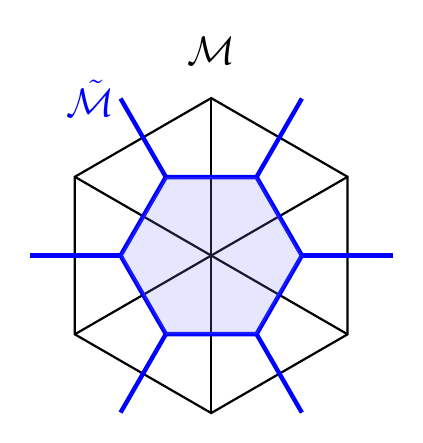
\begin{tikzpicture}
    \def\primalstyle{thick}
    \def\dualstyle{ultra thick}
    \coordinate (P0) at (0cm, 0cm);
    \foreach \i in {1,2,...,6}
    {
    \coordinate (P\i) at ({60*\i-30}:2cm);
    \draw[\primalstyle] (P0) -- (P\i);
    }
    \draw[\primalstyle] (P1) -- (P2) node[above=3mm]{\Large $\mathcal{M}$} node[left=11mm]{\Large \color{blue} $\Tilde{\mathcal{M}}$} -- (P3) -- (P4) -- (P5) -- (P6) -- cycle;
    \foreach \i in {1,2,...,6}
    {
    \coordinate (D\i) at ({60*\i-60}:{2./1.737});
    \coordinate (DD\i) at ({60*\i-60}:{4./1.737});
    }
    \draw[blue,\dualstyle] (D1) -- (D2) -- (D3) -- (D4) -- (D5) -- (D6) -- cycle;
    \foreach \i in {1,2,...,6}
    {
    \draw[blue,\dualstyle] (D\i) -- (DD\i);
    }
    \fill[blue!50, opacity=0.2] (D1) -- (D2) -- (D3) -- (D4) -- (D5) -- (D6) -- cycle;
    \end{tikzpicture}}
    \caption{2D case}
    \label{fig:2d-mesh}
    \end{subfigure}
    \begin{subfigure}[b]{0.45\textwidth}
    \centering
    \resizebox{0.8\textwidth}{!}{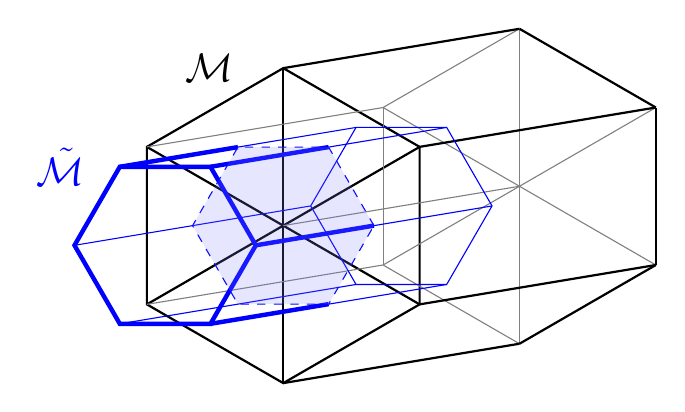
\begin{tikzpicture}
    \def\primalstyle{thick}
    \def\dualstyle{thick}
    \coordinate (P0) at (0cm, 0cm);
    \foreach \i in {1,2,...,6}
    {
    \coordinate (P\i) at ({60*\i-30}:2cm);
    \draw[\primalstyle] (P0) -- (P\i);
    }
    \draw[\primalstyle] (P1) -- (P2) node[left=5mm]{\Large $\mathcal{M}$} -- (P3) -- (P4) -- (P5) -- (P6) -- cycle;
    \begin{scope}[shift={(3cm,0.5cm)}]
        \coordinate (PP0) at (0cm, 0cm);
        \foreach \i in {1,2,...,6}
        {
        \coordinate (PP\i) at ({60*\i-30}:2cm);
        \draw[gray] (PP0) -- (PP\i);
        }
    \end{scope}
    
    \draw[\primalstyle] (PP1) -- (PP2);
    \draw[gray] (PP2) -- (PP3);
    \draw[gray] (PP3) -- (PP4);
    \draw[gray] (PP4) -- (PP5);
    \draw[\primalstyle] (PP5) -- (PP6);
    \draw[\primalstyle] (PP6) -- (PP1);
    
    \draw[gray] (P0) -- (PP0);
    \draw[\primalstyle] (P1) -- (PP1);
    \draw[\primalstyle] (P2) -- (PP2);
    \draw[gray] (P3) -- (PP3);
    \draw[gray] (P4) -- (PP4);
    \draw[\primalstyle] (P5) -- (PP5);
    \draw[\primalstyle] (P6) -- (PP6);
    
    \foreach \i in {1,2,...,6}
    {
    \coordinate (D\i) at ({60*\i-60}:{2./1.737});
    }
    \draw[dashed, blue] (D1) -- (D2) -- (D3) -- (D4) -- (D5) -- (D6) -- cycle;
    \begin{scope}[shift={(1.5,0.25)}]
        \foreach \i in {1,2,...,6}
        {
        \coordinate (DD\i) at ({60*\i-60}:{2./1.737});
        }
    \end{scope}
    \draw[blue] (DD1) -- (DD2) -- (DD3) -- (DD4) -- (DD5) -- (DD6) -- cycle;
    \draw[blue] (D1) -- (DD1);
    \draw[blue] (D2) -- (DD2);
    \draw[blue] (D3) -- (DD3);
    \draw[blue] (D4) -- (DD4);
    \draw[blue] (D5) -- (DD5);
    \draw[blue] (D6) -- (DD6);
    
    \begin{scope}[shift={(-1.5,-0.25)}]
        \foreach \i in {1,2,...,6}
        {
        \coordinate (DDD\i) at ({60*\i-60}:{2./1.737});
        }
    \end{scope}
    \draw[blue, ultra thick] (DDD1) -- (DDD2) -- (DDD3) node[left=3mm]{\textcolor{blue}{\Large $\Tilde{\mathcal{M}}$}} -- (DDD4) -- (DDD5) -- (DDD6) -- cycle;
    \draw[blue, ultra thick] (D1) -- (DDD1);
    \draw[blue, ultra thick] (D2) -- (DDD2);
    \draw[blue, ultra thick] (D3) -- (DDD3);
    \draw[blue] (D4) -- (DDD4);
    \draw[blue] (D5) -- (DDD5);
    \draw[blue, ultra thick] (D6) -- (DDD6);
    
    \fill[blue!50, opacity=0.2] (D1) -- (D2) -- (D3) -- (D4) -- (D5) -- (D6);
    
    \end{tikzpicture}}
    \caption{3D case (2D extrusion)}
    \label{fig:2d-extrusion}
    \end{subfigure}
    \hfill
    \caption{Illustration of primal and dual meshes. (a) A Delaunay-Voronoi grid in 2D (b) The extrusion of 2D mesh. Six triangle prisms are primal cells (depicted by black and gray edges). One dual cell, which is a hexagon prism, is depicted by blue edges. The dashed hexagon represents the intersection of the dual cell and primal cells.}
    \label{fig:illustration_primal_dual}
\end{figure}

\subsubsection{Orientation and Incidence Matrices}
Each geometrical element in the primal mesh $\mathcal{M}$ is (arbitrarily) endowed of an \emph{internal orientation} \footnote{This notion should not be aliased with \emph{inner orientation}, which has a slightly different definition, see \cite{tonti_2002}.}. The notion is sketched in Fig. \ref{fig:orientation}. For the elements of the dual mesh $\Tilde{\mathcal{M}}$, we set their internal orientations to be aligned with their corresponding primal elements according to the bijective mappings.

Another orientation attribute, \emph{induced orientation}, is defined as follows: an induced orientation of a k-dim element $f$ with respect to a (k+1)-dim element $f'$, satisfying $f \subset \partial f' $, is determined by the internal orientation of $f'$ according to the rule shown in Fig. \ref{fig:orientation}. 

These information can be formulated into matrices with entries in $\{0,-1,+1\}$, called \emph{incidence matrices}. To describe the primal face-to-edge relation, for instance, a sparse matrix $\mathbb{C} \in \mathbb{R}^{N_A \times N_L}$ is assembled whose $(i,j)$-entry is assigned $+1$ if the internal orientation of edge $L_j$ and its induced orientation with respect to face $A_i$ coincides; it is assigned $-1$ if two orientations are opposite; and assigned $0$ if $L_j$ is not a subset of the boundary of $A_i$. One would see in the later section that $\mathbb{C}$ functions as a discrete version of curl operator. The other incidence matrices are constructed in the same manner, see Tab. \ref{tab:incidence_mat} for a summary. Given the link of orientations of $\mathcal{M}$ and $\Tilde{\mathcal{M}}$, we can derive the relations listed in Tab. \ref{tab:incidence_relation}.  

\begin{table}[h!]
    \centering
    \begin{tabular}{c c c c}
    \hline
         Matrix & Size & Incidence relation & Intuition  \\
    \hline
         $\mathbb{D}\ (\Tilde{\mathbb{D}})$ & $N_V \times N_A\ (N_{\Tilde{V}} \times N_{\Tilde{A}})$ & volume $\rightarrow$ face & discrete div \\
         $\mathbb{C}\ (\Tilde{\mathbb{C}})$ & $N_A \times N_L\ (N_{\Tilde{A}} \times N_{\Tilde{L}})$ & face $\rightarrow$ edge & discrete curl \\
         $\mathbb{G}\ (\Tilde{\mathbb{G}})$ & $N_L \times N_P\ (N_{\Tilde{L}} \times N_{\Tilde{P}})$ & edge $\rightarrow$ vertex & discrete grad \\
    \hline
    \end{tabular}
    \caption{Summary of incidence matrices}
    \label{tab:incidence_mat}
\end{table}

\begin{table}[h!]
    \centering
    \begin{tabular}{l c}
    \hline
         Relation & Intuition \\
    \hline
         $\mathbb{G}^T = -\Tilde{\mathbb{D}}$  &  $\text{grad}^* = - \text{div}$\\
         $\mathbb{C}^T = \Tilde{\mathbb{C}}$   &  $\text{curl}^* = - \text{curl}$\\
         $\mathbb{D}^T = -\Tilde{\mathbb{G}}$  &  $\text{div}^* = - \text{grad}$\\
         $\mathbb{C}\mathbb{G} = \mathbf{0}, \Tilde{\mathbb{C}}\Tilde{\mathbb{G}} = \mathbf{0}$  &  curl $\circ$ grad = 0 \\
         $\mathbb{D}\mathbb{C} = \mathbf{0}, \Tilde{\mathbb{D}}\Tilde{\mathbb{C}} = \mathbf{0}$   &  div $\circ$ curl = 0 \\
    \hline
        \small $\ast$ denotes adjoint operator.
    \end{tabular}
    \caption{Relations between incidence matrices}
    \label{tab:incidence_relation}
\end{table}

These matrices are topological and thus invariant under smooth deformation of the domain. In the next section, we will show that they play a crucial role in constructing the topological relations of the unknowns. 

\begin{figure}
    \centering
    \begin{minipage}{0.2\textwidth}
    \centering
    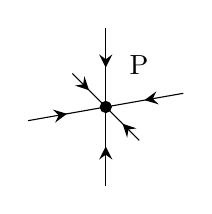
\begin{tikzpicture}
        \coordinate (P0) at (0,0);
        \coordinate (P1) at (10:1); 
        \coordinate (P2) at (90:1);
        \coordinate (P3) at (190:1);
        \coordinate (P4) at (270:1);
        \coordinate (P5) at (135:0.6);
        \coordinate (P6) at (-45:0.6);
        \foreach \i in {1,2,...,6} 
        {
            \draw[decoration={markings, mark= at position 0.5 with {\arrow[scale=1.5]{stealth}}},postaction={decorate}] (P\i) -- (P0);
        }
        \draw[fill=black] (P0) circle (0.07) node[yshift=15pt, xshift=12pt]{P}; 
    \end{tikzpicture}
    \end{minipage}
    \begin{minipage}{0.2\textwidth}
    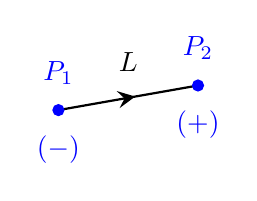
\begin{tikzpicture}
        \coordinate (P1) at (0,0);
        \coordinate (P2) at (10:1.8);
        \draw[decoration={markings, mark= at position 0.55 with {\arrow[scale=1.5]{stealth}}},postaction={decorate}, thick] (P1) -- node[above=2mm]{$L$} (P2);
        \draw[blue, fill=blue] (P1) circle (0.07) node[above=2mm] {\color{blue}$P_1$} node[below=2mm] {\color{blue}$(-)$};
        \draw[blue, fill=blue] (P2) circle (0.07) node[above=2mm] {\color{blue}$P_2$} node[below=2mm] {\color{blue}$(+)$};
    \end{tikzpicture}
    \end{minipage}
    \begin{minipage}{0.2\textwidth}
    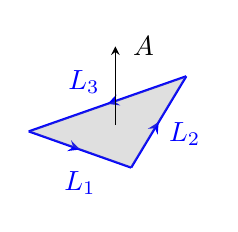
\begin{tikzpicture}
        \coordinate (Q1) at (0,0);
        \coordinate (Q2) at (1.3cm, -0.46cm);
        \coordinate (Q3) at (2.0cm, 0.7cm);
        \draw[decoration={markings, mark= at position 0.5 with {\arrow[scale=1]{stealth}}}, postaction={decorate}, thick, blue] (Q1) -- node[below=1.5mm]{$L_1$} (Q2);
        \draw[decoration={markings, mark= at position 0.5 with {\arrow[scale=1]{stealth}}}, postaction={decorate},  thick, blue] (Q2) -- node[right,yshift=-1.5mm]{$L_2$} (Q3);
        \draw[decoration={markings, mark= at position 0.5 with {\arrow[scale=1]{stealth}}}, postaction={decorate},  thick, blue] (Q3) -- node[above,xshift=-3mm] {$L_3$}(Q1);
        \fill[black!50, opacity=0.25] (Q1) -- (Q2) -- (Q3);
        \draw[-stealth](barycentric cs:Q1=1,Q2=1,Q3=1) -- ([shift={(0,1cm)}] barycentric cs:Q1=1,Q2=1,Q3=1) node[right,xshift=1mm] {$A$}; 
    \end{tikzpicture}
    \end{minipage}
    \begin{minipage}{0.2\textwidth}
    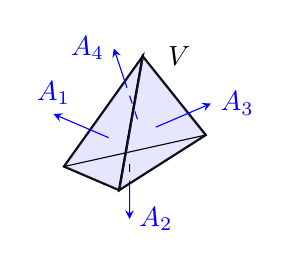
\begin{tikzpicture}
        \coordinate (S1) at (0,0);
        \coordinate (S2) at (-0.7,0.3);
        \coordinate (S3) at (1.1,0.7);
        \coordinate (S4) at (0.3,1.7);
        \draw[thick] (S1) -- (S2) -- (S4) -- cycle;
        \fill[blue!50, opacity=0.2] (S1) -- (S2) -- (S4);
        \draw[thick] (S1) -- (S3) -- (S4) -- cycle;
        \fill[blue!50, opacity=0.2] (S1) -- (S3) -- (S4);
        \draw[thin] (S2) -- (S3);
        \draw[-stealth, blue] (barycentric cs:S1=1,S2=1,S4=1) -- ([shift={(-0.7,0.3)}] barycentric cs:S1=1,S2=1,S4=1) node[above] {$A_1$};
        \coordinate (O1) at (barycentric cs:S1=1,S2=1,S3=1);
        \coordinate (O2) at ([shift={(0,-0.7)}] barycentric cs:S1=1,S2=1,S3=1);
        \coordinate (S)  at (intersection of O1--O2 and S1--S3);
        \draw[dashed] (O1) -- (S);
        \draw[-stealth, blue] (S) -- (O2) node[right] {$A_2$};
        \draw[-stealth, blue] (barycentric cs:S1=1,S3=1,S4=1) -- ([shift={(0.7,0.3)}] barycentric cs:S1=1,S3=1,S4=1) node[right] {$A_3$} ;
        \coordinate (OO1) at (barycentric cs:S2=1,S3=1,S4=1);
        \coordinate (OO2) at ([shift={(-0.3,0.9)}] barycentric cs:S2=1,S3=1,S4=1);
        \coordinate (SS)  at (intersection of OO1--OO2 and S2--S4);
        \draw[dashed, blue] (OO1) -- (SS);
        \draw[-stealth, blue] (SS) -- (OO2) node[left] {$A_4$};
        \node at (S4) [right, xshift=2mm] {$V$};
    \end{tikzpicture}
    \end{minipage}
    \caption{Illustration of internal and induced orientations. The internal orientation of each element is depicted in black color: vertices are oriented as \emph{sink} by default; edges are oriented by their pointing direction; faces are oriented by their normal vector; volumes are oriented as positive default. The induced orientations are depicted in blue color: the ending vertex of an edge is negatively oriented while the starting point is positively oriented; the orientations of edges with respect to a face obey the right-hand rule; a face of a volume are oriented by its outer normal vector. }
    \label{fig:orientation}
\end{figure}

\subsubsection{Cut-off Boundary}
In simulations, the meshes are confined by a definite boundary. To make them aligned at boundary, we have to cut off the \emph{dual} elements near the boundary due to the staggered character. In the meantime, extra elements are needed to close $\Tilde{\mathcal{M}}$. These issues are illustrated in Fig. \ref{fig:illustraion_dual_boundary}.

Note that the auxiliary edges might not be straight and the auxiliary faces might not be flat, which necessitates a versatile data structure to include such situations. In the following, the auxiliary elements would be treated as dual elements, which limits the validity of the relations in Tab. \ref{tab:incidence_relation} only for interior part of $\Tilde{\mathcal{M}}$.

\begin{figure}
    \begin{subfigure}[b]{0.3\textwidth}
        \centering
        \begin{tikzpicture}
            \colorlet{dual}{blue}
            \tkzDefPoint(0,0){P1} 
            \tkzDefPoint(1,1){P1}
            \tkzDefPoint(1.1,-0.8){P2} 
            \tkzDefPoint(0.4,-1.4){P3} 
            \tkzDefPoint(2,0.9){P4} 
            \tkzDefPoint(1.4, 0){P5}
            \tkzDefPoint(2.3, 0){P6}
            \tkzDefPoint(2.1,-1){P7} 
            \tkzDefPoint(1.6,-1.7){P8} 
            \foreach \i in {0,...,8} {\tkzDrawPoints(P\i)}
            %\foreach \i in {0,...,8} {\tkzLabelPoints(P\i)}
            \tkzDrawSegments(P1,P0 P1,P4 P1,P5 P5,P0 P5,P4 P5,P2 P5,P6 P4,P6 P0,P2 P2,P7 P5,P7 P6,P7 P3,P0 P3,P2 P3,P8 P2,P8 P8,P7)
            \tkzDefTriangleCenter[circum](P1,P0,P5) \tkzGetPoint{O1} 
            \tkzDefTriangleCenter[circum](P1,P4,P5) \tkzGetPoint{O2}
            \tkzDefTriangleCenter[circum](P4,P6,P5) \tkzGetPoint{O3}
            \tkzDefTriangleCenter[circum](P2,P0,P5) \tkzGetPoint{O4} 
            \tkzDefTriangleCenter[circum](P2,P7,P5) \tkzGetPoint{O5}
            \tkzDefTriangleCenter[circum](P2,P0,P3) \tkzGetPoint{O6}
            \tkzDefTriangleCenter[circum](P2,P3,P8) \tkzGetPoint{O7}
            \tkzDefTriangleCenter[circum](P2,P7,P8) \tkzGetPoint{O8}
            \tkzDefTriangleCenter[circum](P5,P6,P7) \tkzGetPoint{O9}
            \foreach \i in {1,...,9} {\tkzDrawPoints[dual](O\i)}
            %\foreach \i in {1,...,9} {\tkzLabelPoints(O\i)}
            \tkzDrawSegments[dual](O1,O2 O2,O3 O3,O9 O9,O5 O5,O4 O1,O4 O4,O6 O6,O7 O7,O8 O8,O5 O5,O9)
            \tkzDefMidPoint(P0,P1) \tkzGetPoint{M0} \tkzDrawSegment[dual, add= 0 and 1](O1, M0)
            \tkzDefMidPoint(P1,P4) \tkzGetPoint{M1} \tkzDrawSegment[dual, add= 0 and 1](O2, M1)
            \tkzDefMidPoint(P4,P6) \tkzGetPoint{M2} \tkzDrawSegment[dual, add= 0 and 1](O3, M2)
            \tkzDefMidPoint(P6,P7) \tkzGetPoint{M3} \tkzDrawSegment[dual, add= 0 and 1](O9, M3)
            \tkzDefMidPoint(P7,P8) \tkzGetPoint{M4} \tkzDrawSegment[dual, add= 0 and 1](O8, M4)
            \tkzDefMidPoint(P3,P8) \tkzGetPoint{M5} \tkzDrawSegment[dual, add= 0 and 1](O7, M5)
            \tkzDefMidPoint(P0,P3) \tkzGetPoint{M6} \tkzDrawSegment[dual, add= 0 and 1](O6, M6)
        \end{tikzpicture}
        \caption{Before cut-off}
    \end{subfigure}
    \begin{subfigure}[b]{0.3\textwidth}
        \centering
        \begin{tikzpicture}
            \colorlet{dual}{blue}
            \colorlet{aux}{orange}
            \tkzDefPoint(0,0){P1} 
            \tkzDefPoint(1,1){P1}
            \tkzDefPoint(1.1,-0.8){P2} 
            \tkzDefPoint(0.4,-1.4){P3} 
            \tkzDefPoint(2,0.9){P4} 
            \tkzDefPoint(1.4, 0){P5}
            \tkzDefPoint(2.3, 0){P6}
            \tkzDefPoint(2.1,-1){P7} 
            \tkzDefPoint(1.6,-1.7){P8} 
            \foreach \i in {0,...,8} {\tkzDrawPoints(P\i)}
            %\foreach \i in {0,...,8} {\tkzLabelPoints(P\i)}
            \tkzDrawSegments(P1,P0 P1,P4 P1,P5 P5,P0 P5,P4 P5,P2 P5,P6 P4,P6 P0,P2 P2,P7 P5,P7 P6,P7 P3,P0 P3,P2 P3,P8 P2,P8 P8,P7)
            \tkzDefTriangleCenter[circum](P1,P0,P5) \tkzGetPoint{O1} 
            \tkzDefTriangleCenter[circum](P1,P4,P5) \tkzGetPoint{O2}
            \tkzDefTriangleCenter[circum](P4,P6,P5) \tkzGetPoint{O3}
            \tkzDefTriangleCenter[circum](P2,P0,P5) \tkzGetPoint{O4} 
            \tkzDefTriangleCenter[circum](P2,P7,P5) \tkzGetPoint{O5}
            \tkzDefTriangleCenter[circum](P2,P0,P3) \tkzGetPoint{O6}
            \tkzDefTriangleCenter[circum](P2,P3,P8) \tkzGetPoint{O7}
            \tkzDefTriangleCenter[circum](P2,P7,P8) \tkzGetPoint{O8}
            \tkzDefTriangleCenter[circum](P5,P6,P7) \tkzGetPoint{O9}
            \foreach \i in {1,...,9} {\tkzDrawPoints[dual](O\i)}
            %\foreach \i in {1,...,9} {\tkzLabelPoints(O\i)}
            \tkzDrawSegments[dual](O1,O2 O2,O3 O3,O9 O9,O5 O5,O4 O1,O4 O4,O6 O6,O7 O7,O8 O8,O5 O5,O9)
            \tkzDefMidPoint(P0,P1) \tkzGetPoint{M0} \tkzDrawSegment[dual](O1, M0)
            \tkzDefMidPoint(P1,P4) \tkzGetPoint{M1} \tkzDrawSegment[dual](O2, M1)
            \tkzDefMidPoint(P4,P6) \tkzGetPoint{M2} \tkzDrawSegment[dual](O3, M2)
            \tkzDefMidPoint(P6,P7) \tkzGetPoint{M3} \tkzDrawSegment[dual](O9, M3)
            \tkzDefMidPoint(P7,P8) \tkzGetPoint{M4} \tkzDrawSegment[dual](O8, M4)
            \tkzDefMidPoint(P3,P8) \tkzGetPoint{M5} \tkzDrawSegment[dual](O7, M5)
            \tkzDefMidPoint(P0,P3) \tkzGetPoint{M6} \tkzDrawSegment[dual](O6, M6)
            %\foreach \i in {0,...,6} {\tkzLabelPoints(M\i)}
            
            \tkzDefPointWith[K=1.2, linear](O1,M0) \tkzGetPoint{N0} 
            \tkzDefPointWith[K=1.2, linear](O2,M1) \tkzGetPoint{N1}
            \tkzDefPointWith[K=1.2, linear](O3,M2) \tkzGetPoint{N2}
            \tkzDefPointWith[K=1.2, linear](O9,M3) \tkzGetPoint{N3}
            \tkzDefPointWith[K=1.2, linear](O8,M4) \tkzGetPoint{N4}
            \tkzDefPointWith[K=1.5, linear](O7,M5) \tkzGetPoint{N5}
            \tkzDefPointWith[K=1.4, linear](O6,M6) \tkzGetPoint{N6}
            \foreach \i in {0,...,6} {\tkzDrawPoints[aux](N\i)}
            
            \tkzDefPointWith[K=1.07, linear](P5,P1) \tkzGetPoint{PP1}
            \tkzDefPointWith[K=1.07, linear](P5,P4) \tkzGetPoint{PP4}
            \tkzDefPointWith[K=1.08, linear](P5,P6) \tkzGetPoint{PP6}
            \tkzDefPointWith[K=1.07, linear](P2,P7) \tkzGetPoint{PP7}
            \tkzDefPointWith[K=1.07, linear](P2,P8) \tkzGetPoint{PP8}
            \tkzDefPointWith[K=1.07, linear](P2,P3) \tkzGetPoint{PP3}
            \tkzDefPointWith[K=1.03, linear](M3,P0) \tkzGetPoint{PP0}
            
            \tkzDrawSegments[aux](N0,PP1 PP1,N1 N1,PP4 PP4,N2 N2,PP6 PP6,N3 N3,PP7 PP7,N4 N4,PP8 PP8,N5 N5,PP3 PP3,N6 N6,PP0 PP0,N0)
            
        \end{tikzpicture}
    \caption{After cut-off}
    \end{subfigure}
    \begin{subfigure}[b]{0.35\textwidth}
        \centering
        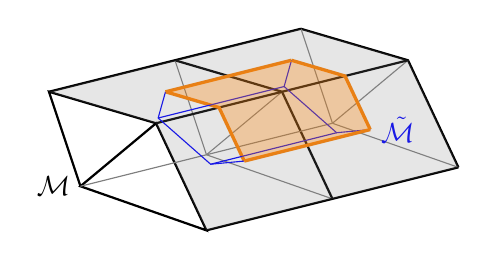
\begin{tikzpicture}[scale=0.8]
            \coordinate (A1) at (0,0);
            \coordinate (A2) at (2,-0.7);
            \coordinate (A3) at (1.2,1);
            \coordinate (A4) at (-0.5,1.5);
            \draw[thick] (A1) node[left] {$\mathcal{M}$} -- (A2) -- (A3) -- cycle;
            \draw[thick] (A1) -- (A4) -- (A3);
            \begin{scope}[shift={(2,0.5)}]
                \coordinate (B1) at (0,0);
                \coordinate (B2) at (2,-0.7);
                \coordinate (B3) at (1.2,1);
                \coordinate (B4) at (-0.5,1.5);
                \draw[thick] (B2) -- (B3) -- (B4);
                \draw[gray]  (B1) -- (B3);
                \draw[gray]  (B1) -- (B2);
                \draw[gray]  (B1) -- (B4);
            \end{scope}
            \begin{scope}[shift={(4,1)}]
                \coordinate (C1) at (0,0);
                \coordinate (C2) at (2,-0.7);
                \coordinate (C3) at (1.2,1);
                \coordinate (C4) at (-0.5,1.5);
                \draw[thick] (C2) -- (C3) -- (C4);
                \draw[gray]  (C1) -- (C3);
                \draw[gray]  (C1) -- (C2);
                \draw[gray]  (C1) -- (C4);
            \end{scope}
            \draw[thick] (A4) -- (B4) -- (C4);
            \draw[thick] (A3) -- (B3) -- (C3);
            \draw[thick] (A2) -- (B2) -- (C2);
            \draw[gray]  (A1) -- (C1);
            \coordinate (O1) at (barycentric cs:A3=1,B3=1);
            \coordinate (O2) at (barycentric cs:A3=1,B3=1,A4=1,B4=1);
            \coordinate (O5) at (barycentric cs:A3=1,B3=1,A2=1,B2=1);
            \draw[orange, very thick] (O2) -- (O1) -- (O5);
            \coordinate (O3) at (barycentric cs:A1=1,A3=1,A4=1,B1=1,B3=1,B4=1);
            \coordinate (O4) at (barycentric cs:A1=1,A2=1,A3=1,B1=1,B2=1,B3=1);
            \draw[blue] (O2) -- (O3) -- (O4) -- (O5);
            \coordinate (OO1) at ([shift={(2,0.5)}]O1);
            \coordinate (OO2) at ([shift={(2,0.5)}]O2);
            \coordinate (OO3) at ([shift={(2,0.5)}]O3);
            \coordinate (OO4) at ([shift={(2,0.5)}]O4);
            \coordinate (OO5) at ([shift={(2,0.5)}]O5);
            \draw[very thick, orange] (OO2) -- (OO1) -- (OO5) node[right] {\textcolor{blue}{$\Tilde{\mathcal{M}}$}};
            \draw[blue] (OO2) -- (OO3) -- (OO4) -- (OO5);
            \draw[very thick, orange] (O2) -- (OO2);
            %\draw[very thick, blue] (O1) -- (OO1);
            \draw[very thick, orange] (O5) -- (OO5);
            \draw[blue] (O3) -- (OO3);
            \draw[blue] (O4) -- (OO4);
            \fill[gray,opacity=0.2] (A4) -- (A3) -- (C3) -- (C4);
            \fill[gray,opacity=0.2] (A3) -- (A2) -- (C2) -- (C3);
            \fill[orange,opacity=0.3] (OO2)--(O2)--(O1)--(O5)--(OO5)--(OO1);
        \end{tikzpicture}
        \caption{3D case}
    \end{subfigure}
    \caption{Illustration of cut-off boundary. Before the cut-off, the boundary of $\Tilde{\mathcal{M}}$ is not well-defined. To resolve the same boundary as $\mathcal{M}$, boundary dual volumes are truncated and auxiliary elements are supplemented (shown in orange color). To be specific, in subfigure (c) four edges and one face are added in order to close this dual volume. Notice that these auxiliary edges and faces can be non-straight and non-flat.}
    \label{fig:illustraion_dual_boundary}
\end{figure}

\subsection{Discrete Maxwell Equations}
\subsubsection{The Finite Integration Technique (FIT)}
We utilize the FIT to discretize Maxwell's equations. This framework was originally proposed in \cite{weiland_1977} and can be treated as a generalization of Yee's FDTD method \cite{yee_1966}. FIT is established based on the integral form of Maxwell's equations:
\begin{subequations}
\begin{align}
    &\oint_{\partial A} \mathbf{E} \cdot d\mathbf{s} \ = - \iint_A \frac{\partial \mathbf{B}}{\partial t} \cdot d\mathbf{A}, \label{equ:maxwell_int_faraday}\\
    &\oint_{\partial A} \mathbf{H} \cdot d\mathbf{s} \ = \iint_A \left(\frac{\partial \mathbf{D}}{\partial t} + \mathbf{J}\right) \cdot d\mathbf{A}, \label{equ:maxwell_int_ampere}\\
    &\oint_{\partial V} \mathbf{B} \cdot d\mathbf{A} = 0, \label{equ:maxwell_int_gauss_B}\\
    &\oint_{\partial V} \mathbf{D} \cdot d\mathbf{A} = \iiint_V \rho dV. \label{equ:maxwell_int_gauss_D}
\end{align}
\end{subequations}
where $A, V$ stand for arbitrary surfaces and volumes in the spatial domain. 

Given the mesh pair $(\mathcal{M}, \Tilde{\mathcal{M}})$, the discrete Maxwell system is described by applying the integral equations (\ref{equ:maxwell_int_faraday})-(\ref{equ:maxwell_int_gauss_D}) to the elements in $(\mathcal{M}, \Tilde{\mathcal{M}})$. We end up with
\begin{subequations}
\begin{align}
    &\sum_{j:L_j\in\partial A_i} \underbrace{\int_{L_j} \mathbf{E} \cdot d\mathbf{s}}_{e_j} = - \frac{\partial}{\partial t} \underbrace{\iint_{A_i} \mathbf{B} \cdot d\mathbf{A}}_{b_i},\ \ \ i = 1,...,N_A, \label{equ:maxwell_grid_faraday} \\
    &\sum_{j:\Tilde{L}_j\in\partial \Tilde{A}_i} \underbrace{\int_{\Tilde{L}_j} \mathbf{H} \cdot d\mathbf{s}}_{h_j} = \frac{\partial}{\partial t} \underbrace{\iint_{\Tilde{A}_i} \mathbf{D} \cdot d\mathbf{A}}_{d_i} + \underbrace{\iint_{\Tilde{A}_i} \mathbf{J} \cdot d\mathbf{A}}_{j_i}, \ \ \ i = 1,...,N_{\Tilde{A}}, \label{equ:maxwell_grid_ampere}\\
    &\sum_{j:A_j\in \partial V_i} \iint_{A_j} \mathbf{B} \cdot d\mathbf{A} = 0,\ \ \ i = 1,..., N_V,\label{equ:maxwell_grid_gauss_B}\\
    &\sum_{j:\Tilde{A}_j \in \partial\Tilde{V}_i}\iint_{\Tilde{A}_j} \mathbf{D} \cdot d\mathbf{A} = \underbrace{\iiint_{\Tilde{V}_i} \rho dV}_{q_i},\ \ \ i = 1,...,N_{\Tilde{V}}. \label{equ:maxwell_grid_gauss_D}
\end{align}
\end{subequations}
where $i, j$ are indices for elements in the meshes.

The integral quantities are the unknowns to be solved. As is defined in (\ref{equ:maxwell_grid_faraday})-(\ref{equ:maxwell_grid_gauss_D}) by the underbraces, these scalar quantities are stacked into vectors:
\begin{equation} \label{equ:fit_scale_vector}
    \mathbf{e} := (e_i)_{i=1}^{N_L},\ \ \mathbf{b} := (b_i)_{i=1}^{N_A}, \ \ \mathbf{h} := (h_i)_{i=1}^{N_{\Tilde{L}}}, \ \ \mathbf{d} := (d_i)_{i=1}^{N_{\Tilde{A}}}, \ \ \mathbf{j} := (j_i)_{i=1}^{N_{\Tilde{A}}}, \ \ \mathbf{q} := (q_i)_{i=1}^{N_{\Tilde{V}}}.
\end{equation}

The material laws (\ref{equ:material_law}) need to be reformulated within this framework. The relations between scalar vectors, in the form of $\mathbf{b} = \mathbb{M}_\mu \mathbf{h}$ and $\mathbf{d} = \mathbb{M}_\varepsilon \mathbf{e}$, are to be derived. In the simplest case where permittivity $\mu$ and permeability $\varepsilon$ are homogeneous in the domain, and the orthogonality of ($\mathcal{M}, \Tilde{\mathcal{M}}$) pair is ensured, the material matrices are diagonal with entries 

\begin{equation*}
    (\mathbb{M}_\mu)_{i,i} = \frac{\mu|A_i|}{|\Tilde{L}_i|}, \ \ \ \ \ (\mathbb{M}_\varepsilon)_{i,i} = \frac{\varepsilon |\Tilde{A}_i|}{|L_i|},
\end{equation*}
where $|\cdot|$ denotes taking length or area. We would like to remark that the approximation error is introduced due to the implicit assumption that vector fields are piecewise constant, see analysis in \cite{Marrone_2001}.

With the aid of incidence matrices defined in the preceding section and given the discrete material law, (\ref{equ:maxwell_grid_faraday})-(\ref{equ:maxwell_grid_gauss_D}) can be reformulated by a set of algebraic equations:
\begin{center}
\vspace{-0.5cm}
\begin{minipage}{0.3\textwidth}
\begin{align*}
    \partial_t \mathbf{B} + \nabla \times \mathbf{E} &= 0, \\
    \partial_t \mathbf{D} - \nabla \times \mathbf{H} &= -\mathbf{J}, \\
    \nabla \cdot \mathbf{B} &= 0,  \\
    \nabla \cdot \mathbf{D} &= \rho, \\
    \mathbf{H} &= \mu^{-1} \mathbf{B}, \\
    \mathbf{D} &= \varepsilon \mathbf{E}. 
\end{align*}
\end{minipage}
\begin{minipage}{0.1\textwidth}
\centering
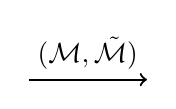
\begin{tikzpicture}
\draw[thick, -{to}] (0,0) -- node[above]{$(\mathcal{M}, \Tilde{\mathcal{M}})$} (1.5,0);
\end{tikzpicture}
\end{minipage}
\begin{minipage}{0.3\textwidth}
\begin{subequations}
\begin{align}
    \dot{\mathbf{b}} + \mathbb{C}\mathbf{e} &= \mathbf{0} , \label{equ:alg_faraday}\\
    \dot{\mathbf{d}} - \Tilde{\mathbb{C}}\mathbf{h} &= - \mathbf{j}, \label{equ:alg_empere}\\
    \mathbb{D}\mathbf{b} &= \mathbf{0},  \label{equ:alg_gauss_b}\\
    \Tilde{\mathbb{D}}\mathbf{d} &= \mathbf{q},  \label{equ:alg_gauss_d}\\
    \mathbf{h} &= \mathbb{M}_\mu^{-1} \mathbf{b}, \label{equ:alg_material_magnetic}\\
    \mathbf{d} &= \mathbb{M}_{\varepsilon} \mathbf{e}, \label{equ:alg_material_electric} 
\end{align}
\end{subequations}
\end{minipage}
\end{center}
where the topping dot $\cdot$ stands for time derivative.

At this point, we would like to emphasis the importance of the primal-dual staggered meshes: the material laws can be included in a rather simple way. For magnetic Gauss's law $\mathbf{D} = \varepsilon \mathbf{E}$, for instance, the $\mathbf{D}$-field is represented by a collection of face integrals $ (d_i)_{i}$ while $\mathbf{E}$-field is represented by a collection of edge integrals $ (e_i)_{i}$. The primal-dual meshes allow us to arrange them in a staggered way -- edges penetrate faces -- such that $\mathbf{D} = \varepsilon \mathbf{E}$ can be approximated by $\mathbf{d} = \mathbb{M}_{\varepsilon}\mathbf{e}$ in a local fashion, namely $\mathbb{M}_{\varepsilon}$ is diagonal. A more schematic illustration involves the language of differential forms and discrete Hodge operator, see \cite{bossavit1999, teixeira_1999, hip_1999}. 

This transformation does not introduce approximations \emph{except for} the discrete material laws. The essence of FIT lies in that the complexity of continuous electric and magnetic field quantities
is reduced to a finite number of well-defined discrete unknowns \citep{weiland_2003}. Also, this discrete version of Maxwell's equations are topological in the sense that they are invariant under different coordinate systems.

\subsubsection{Discrete Boundary Conditions}
The electromagnetic boundary $\Gamma_C, \Gamma_I$ is resolved by the primal mesh $\mathcal{M}$. As is mentioned in Section \ref{sec:BC}, a boundary scalar potential $\Phi$ can be introduced due to the vanishing surface curl of $\mathbf{E}$-field. It holds in the discrete level as well. We assign each primal vertex $P_i \in \partial\Omega$ a scalar value $\varphi_i$. Therefore, the boundary conditions (see Section \ref{sec:BC}) are discretized in the following way:
\begin{center}
    \vspace{-0.5cm}
    \begin{minipage}{0.3\textwidth}
    \begin{align*}
    \varphi = \varphi^\pm(t)\ \ &\text{on} \ \ \Gamma_C^\pm, \\
    \text{curl} \mathbf{E} \cdot \mathbf{n} = 0\ \ &\text{on} \ \  \Gamma_I,  \\
    \text{curl} \mathbf{H} \cdot \mathbf{n} = 0\ \  &\text{on} \ \  \Gamma_I.\
    \end{align*}
    \end{minipage}
    \begin{minipage}{0.1\textwidth}
    \centering
    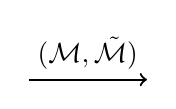
\begin{tikzpicture}
    \draw[thick, -{to}] (0,0) -- node[above]{$(\mathcal{M}, \Tilde{\mathcal{M}})$} (1.5,0);
    \end{tikzpicture}
    \end{minipage}
    \begin{minipage}{0.4\textwidth}
        \begin{subequations}
            \begin{align}
            \varphi_i = \Phi^\pm(t), \ \ &\forall i : P_i \subset \Gamma_C^\pm, \label{equ:bc_1}\\
            e_i = (\mathbb{G}\bm{\varphi})_i,\ \ &\forall i : L_i \subset \partial\Omega, \label{equ:bc_2}\\
            (\Tilde{\mathbb{C}} \bm{h})_i = 0\ \ &\forall i : \Tilde{A}_i \subset \Gamma_I.\label{equ:bc_3}\
            \end{align}
        \end{subequations}
    \end{minipage}
\end{center}

\subsubsection{Reformulation} \label{sec:reform_discrete}
In Section \ref{sec:reform_continuous}, we propose the stabilization of the Maxwell system in the insulating domain $\Omega_I$ by introducing a Lagrange multiplier. In the semi-discrete level, the equations to be solved in $\Omega_I$ are
\begin{subequations}
    \begin{align}
        \dot{\mathbf{b}} + \mathbb{C}\mathbf{e} &= \mathbf{0} ,\\
        \dot{\mathbf{d}} - \Tilde{\mathbb{C}}\mathbf{h} + \colorbox{orange!20}{$\mathbb{H} \mathbb{G} \mathbf{p}$}&= \mathbf{0},\\
        \Tilde{\mathbb{D}}\mathbf{d} &= \mathbf{0} \label{equ:discrete_zero_div}, 
    \end{align} 
\end{subequations}

where $\mathbf{p} = (p_i)_i$ denotes the scalar $p$ assigned to each primal vertex in $\Omega_I$ and the matrix $(\mathbb{H})_{i,i} = \frac{|\Tilde{A}_i|}{|L_i|}$ transforms primal edge integrals to dual face fluxes\footnote{$\mathbb{H}$ functions as a discrete Hodge operator.}. To incorporate the zero Dirichlet BC, we limit the unknowns $(p_i)_{i=1}^{N^{\Omega^\circ_I}_P}$ to primal vertices in the interior of $\Omega_I$.

\subsubsection{An algebraic check on the well-posedness}

We can heuristically examine the well-posedness of the (semi-)discrete Maxwell system by checking whether the numbers of unknowns (also called degrees of freedom (D.o.F.)) and equations coincide. Before counting, we make a meticulous classification for mesh elements according to their locations and summarize the notation for the sake of clarification (see Tab. \ref{tab:def_size_var}). 
\begin{align*}
    \#\  \text{primal cell}\ \  &N_V \\
    \#\  \text{primal edge}\ \  &N_L := \underbrace{N^+_L + N^-_L + N^I_L}_{N^\partial_L} + N^\circ_L  \\
    \#\  \text{primal face}\ \  &N_A := \underbrace{N_A^+ + N_A^- + N^I_A}_{N^\partial_A} + N^\circ_A  \\
    \#\  \text{primal vertex}\ \  &N_P := \underbrace{N_P^+ + N_P^- + N^I_P}_{N^\partial_P} + N^\circ_P \\
    \#\  \text{dual cell}\ \  &N_{\Tilde{V}} := N_P \\
    \#\  \text{dual edge}\ \  &N_{\Tilde{L}} := \underbrace{N^\partial_{\Tilde{L}}}_{=N^\partial_L} + \underbrace{N^\circ_{\Tilde{L}}}_{=N_A} \\
    \#\  \text{dual face}\ \  &N_{\Tilde{A}} := \underbrace{N^\partial_{\Tilde{A}}}_{=N^\partial_P} + \underbrace{N^\circ_{\Tilde{A}}}_{=N_L}
\end{align*}
where the superscripts $\pm, I, \partial, \circ$ indicate that the elements lying in $\gamma^\pm, \gamma^I, \partial\Omega, \Omega^\circ$ respectively . The equations $N^\partial_{\Tilde{L}} = N^\partial_L, N^\partial_{\Tilde{A}} = N^\partial_P$, revealing the bijective relation between the boundary primal elements and auxiliary elements, can be check easily by inspecting Fig. \ref{fig:illustraion_dual_boundary}.

\begin{table}[]
    \centering
\begin{tabular}{c c c}
     \hline
     \textbf{D.o.F.}  & \textbf{Meaning}  & \textbf{Size} \\
     \hline\hline
     $\mathbf{e}$ & line integrals of $\mathbf{E}$-field at primal edges $L$& $N_L$ \\
     $\bm{\varphi}$ & electric potentials at primal vertices $P$ on $\partial\Omega$ & $N_P^\partial$ \\
     $\mathbf{b}$ & surface integrals of $\mathbf{B}$-field at primal faces $A$ & $N_A$ \\
     $\mathbf{h}$ & line integrals of $\mathbf{H}$-field at dual edges $\Tilde{L}$ & $N_{\Tilde{L}}$ \\
     $\mathbf{d}$ & surface integrals of $\mathbf{D}$-field at dual faces $\Tilde{A}$ & $N_{\Tilde{A}}$ \\
     $\mathbf{p}$ & Lagrange multiplier at primal vertices $P$ in $\Omega_I^\circ$ & $N^{\Omega_I^\circ}_P$\\ 
     \hline
\end{tabular}
    \caption{Definitions and sizes of all the degrees of freedom.}
    \label{tab:def_size_var}
\end{table}

Next, we collect all the algebraic equations derived from the Maxwell system and the boundary conditions: 
\begin{align*}
    \text{discrete Faraday law (\ref{equ:alg_faraday})} \ \ &\longrightarrow\ \  N_A \ \ \text{equations} \\
    \text{discrete Ampere law (\ref{equ:alg_empere})} \ \ &\longrightarrow\ \  N_{\Tilde{A}} \ \ \text{equations} \\
    \text{discrete material laws (\ref{equ:alg_material_magnetic})(\ref{equ:alg_material_electric})} \ \ &\longrightarrow\ \  N_A + N_L \ \ \text{equations} \\
    \text{boundary condition (\ref{equ:bc_1})} \ \ &\longrightarrow\ \  N_P^+ + N_P^- \ \ \text{equations} \\
    \text{boundary condition (\ref{equ:bc_2})} \ \ &\longrightarrow\ \  N_L^\partial \ \ \text{equations} \\
    \text{boundary condition (\ref{equ:bc_3})} \ \ &\longrightarrow\ \  N_{\Tilde{A}}^I \ \ \text{equations}. \\
    \text{vanishing divergence constraint (\ref{equ:discrete_zero_div})} \ \ &\longrightarrow\ \  N_P^{\Omega^\circ_I} \ \ \text{equations}. \\
\end{align*}
Comparing the numbers of D.o.F in Tab. \ref{tab:def_size_var} and of the equations we collect, we show that they are equal:
\begin{align*}
    \#\text{ of unknowns} &= \colorbox{violet!20}{$N_L$} + \colorbox{blue!20}{$N_A$} + \colorbox{gray!40}{$N_{\Tilde{L}}$} + \colorbox{orange!20}{$N_{\Tilde{A}}$} + \colorbox{green!20}{$N_P^\partial$} + \colorbox{yellow!40}{$N_P^{\Omega^\circ_I}$}, \\
    \#\text{ of equations} &= \colorbox{blue!20}{$N_A$} + \colorbox{orange!20}{$N_{\Tilde{A}}$} + \colorbox{gray!40}{$N_A$} + \colorbox{violet!20}{$N_L$} + \colorbox{gray!40}{$N_L^\partial$} + \colorbox{green!20}{$N_P^+ + N_P^- + N_P^I$}+ \colorbox{yellow!40}{$N_P^{\Omega^\circ_I}$},
\end{align*}
where the terms with the same color are equal.

However, the matching of numbers of unknowns and equations does not necessarily result in a valid linear system. Inappropriate BCs could cause the singularity of the linear system as $\lambda \rightarrow 0$, which will be discussed later. 

\subsection{Discrete Euler Equations}
We employ the finite volume method (FVM) to discretize the Euler system. As a classical framework for solving conservation laws and hyperbolic systems, FVM is derived from the integral form of the equations in each cell. It is the cell average of quantities that evolves at each time step, based on the \emph{numerical flux} through the cell boundary. The construction of the numerical flux, which serves to approximate the real flux, is the essence of constructing an FVM scheme. Due to the convection nature of fluid dynamics, the numerical fluxes are supposed to respect the convection direction, namely, the \emph{upwind scheme} is preferable. To this end, people resort to the approximated solution of \emph{Riemann problems}. The method is briefly illustrated in the following. For detailed information, see the textbook \cite{leveque_2002}.

The Euler equations (\ref{equ:euler_}) can be generalized into the form of conservation law with source terms:
\begin{equation} \label{equ:euler_conservation}
    \partial_t \mathbf{U} + \nabla \cdot \mathbf{F}(\mathbf{U}) = \mathbf{RHS},
\end{equation}
where $\mathbf{U} \in L^2(\Omega \times [0,T], \mathbb{R}^m)$ stands for $m$ conservative variable, $\mathbf{F}(\mathbf{U}) \in L^2(\Omega \times  [0,T], \mathbb{R}^m)$ is the flux density, and $\mathbf{RHS} \in L^2(\Omega \times  [0,T], \mathbb{R}^m)$ is the source term. 

To obtain the semi-discretization, we first integrate (\ref{equ:euler_conservation}) over a cell $V_i$ 
\begin{equation} \label{equ:euler_grid} 
    \dot{\overline{\mathbf{U}}}_i + \frac{1}{|V_i|}\sum_{j:A_j\in\partial V_i} |A_j|\underbrace{\frac{1}{|A_j|}\iint_{A_j}\mathbf{F}(\mathbf{U})\cdot \mathbf{n}_j \text{d}A}_{\overline{\mathbf{F}}_j} = \underbrace{\frac{1}{|V_i|}\iiint_{V_i} \mathbf{RHS} \text{d}V}_{\overline{\mathbf{RHS}}_i}
\end{equation}
where $\overline{\mathbf{U}}_i := \iiint_{V_i} \mathbf{U} \text{d}V / |V_i| \in L^2([0,T],\mathbb{R}^m)$ calculates the cell average, $\mathbf{n}_j$ is the outer normal vector of face $A_j$ with respect to the cell $V_i$. We approximate the analytic flux $\overline{\mathbf{F}}_j$ in (\ref{equ:euler_grid}) by the numerical flux $\overline{\mathbf{F}}\left(\overline{\mathbf{U}}_i, \overline{\mathbf{U}}_{k(i,j)}, \mathbf{n}_j\right)$, where $k(i,j)$ returns the index of the adjacent cell that shares $A_j$ with cell $V_i$. Classical numerical fluxes include Lax-Friedrich flux, Rusanov flux, Engquist-Osher flux, see \cite[][p. 44-46]{mishra_2019}. Finally, we end up with the semi-discretized equation:
\begin{equation}
    \dot{\overline{\mathbf{U}}}_i + \frac{1}{|V_i|}\sum_{j:A_j\in\partial V_i} |A_j| \overline{\mathbf{F}}\left(\overline{\mathbf{U}}_i, \overline{\mathbf{U}}_{k(i,j)}, \mathbf{n}_j\right) = \overline{\mathbf{RHS}}_i.
    \label{equ:fvm}
\end{equation}
The Rusanov flux in multi-dimensions on face $A_j$ writes
\begin{equation} \label{equ:rusanov-flux-3d}
    \overline{\mathbf{F}}\left(\overline{\mathbf{U}}_L, \overline{\mathbf{U}}_R, \mathbf{n}\right) = \frac{1}{2}\left[\mathbf{F}(\overline{\mathbf{U}}_L)\cdot\mathbf{n} + \mathbf{F}(\overline{\mathbf{U}}_R)\cdot\mathbf{n}\right] - \frac{1}{2}\overline{s}\left(\overline{\mathbf{U}}_R - \overline{\mathbf{U}}_L\right),  
\end{equation}
where $\overline{s} = \text{max}(s(\overline{\mathbf{U}}_L), s(\overline{\mathbf{U}}_R))$ with $s(\mathbf{U}) := |\mathbf{u}\cdot\mathbf{n}| + \sqrt{\gamma p/\rho}$ representing the largest wave speed. 

We would like to emphasis that the Euler system is discretized on $\mathcal{M}'$ due to the fact that 1) the electric current is strongly connected to the momenta of charged particles by (\ref{equ:maxwell_euler_coupling}); 2) the electric current is discretized on dual faces by (\ref{equ:maxwell_grid_ampere}).

To rewrite (\ref{equ:fvm}) into a matrix form, by abuse of notation we stack all the cell average $(\overline{\mathbf{U}}_i)_i$ into a matrix $\mathbf{U} \in \mathbb{R}^{N_{\Tilde{V}}^P \times m}$ with $\mathbf{U}_{i,:} = \overline{\mathbf{U}}_i$. Meanwhile, we denote by $\mathbf{F} \in \mathbb{R}^{N_{\Tilde{A}}^P \times m}$ the collection of the (total) numerical fluxes $|A_i|\overline{\mathbf{F}}_i$, namely $\mathbf{f}_{i,:} = |A_i|\overline{\mathbf{F}}_i$, whose directions are determined by the internal direction of faces where they are defined. In the same way, we denote by $\mathbf{RHS}\in \mathbb{R}^{N_{\Tilde{V}}^P \times m}$ the collection of $\overline{\mathbf{RHS}}_i$. Besides, we define the diagonal matrix $\mathbb{\Tilde{V}} \in \mathbb{R}^{N_{\Tilde{V}}^P}$ with $\mathbb{\Tilde{V}}_{i,i} = |\Tilde{V}_i|$. Making use of the incidence matrices, we end up with
\begin{equation*}
    \dot{\mathbf{U}} + \mathbb{\Tilde{V}}^{-1}\mathbb{\Tilde{D}}\mathbf{F}(\mathbf{U})  = \mathbf{RHS}(\mathbf{U},\mathbf{b},\mathbf{e}),
\end{equation*}
where the dependence of $\mathbf{RHS}$ on $\mathbf{U}, \mathbf{b}, \mathbf{e}$ is implied by (\ref{equ:euler_rescaled}) and will be elaborated below.
\subsubsection{Reconstruction of Lorentz Force}

\subsubsection{Discrete Boundary Conditions}


\subsection{Summary: Spatially Semi-discrete Model}
We collect all the equations and BCs presented above and make a summary for the spatially semi-discrete Maxwell-Euler system:
\begin{subequations}
    \begin{align*}
        [\dot{\mathbf{b}} + \mathbb{C}\mathbf{e} = \mathbf{0}]_i, \ \ &\forall i: A_i \subset \Omega, \\
        [\dot{\mathbf{d}} - \Tilde{\mathbb{C}}\mathbf{h} = - \mathbf{j}]_i, \ \ &\forall i: \Tilde{A}_i \subset \Omega_P,\\
        [\dot{\mathbf{d}} - \Tilde{\mathbb{C}}\mathbf{h} + \mathbb{H} \mathbb{G} \mathbf{p} = - \mathbf{j}]_i, \ \ &\forall i: A_i \subset \Omega_I,\\
        [\Tilde{\mathbb{D}}\mathbf{d} = \mathbf{0}]_i,\ \ &\forall i: \Tilde{V}_i \subset \Omega_I, \\
        [\dot{\mathbf{U}} + \mathbb{\Tilde{V}}^{-1}\mathbb{\Tilde{D}}\mathbf{F} = \mathbf{RHS}]_i,\ \ &\forall i: \Tilde{V}_i \subset \Omega_P,
    \end{align*}
with boundary conditions:
    \begin{align*}
    \varphi_i = \Phi^\pm(t), \ \ &\forall i : P_i \subset \Gamma_C^\pm, \\
    e_i = (\mathbb{G}\bm{\varphi})_i,\ \ &\forall i : L_i \subset \partial\Omega, \\
    (\Tilde{\mathbb{C}} \bm{h})_i = 0,\ \ &\forall i : \Tilde{A}_i \subset \Gamma_I,\\
    \mathbf{F}_i = |\Tilde{A}_i|\overline{\mathbf{F}}(\mathbf{U}_j, \mathbf{U}_j, \mathbf{n}_i), \ \ &\forall i: \Tilde{A}_i \subset \Gamma_C, \\
    \mathbf{F}_i = |\Tilde{A}_i|\overline{\mathbf{F}}(\mathbf{U}_j, \hat{\mathbf{U}}_j, \mathbf{n}_i), \ \ &\forall i: \Tilde{A}_i \subset \Gamma_W.
    \end{align*}
\end{subequations}


\section{Discretization in time}
\subsection{Motivation: 1D Discretization}
\subsubsection{1D plasma model}
The 3D problem is projected onto the 1D axis by assuming vanishing traverse derivatives (see Fig. \ref{fig:1d-frame} for the definition of reference frame). Besides, $u_y, E_y, B_x, B_z$ are set zero for simplicity, which amounts to considering the TE mode. The collision between particles is omitted for the time being. 

Take all the traverse derivatives $\partial_x, \partial_y$ and $u_y, E_y, B_x, B_z$ to be zero, we get the one-fluid Euler-Maxwell system in 1D:
\begin{align*}
    \partial_t n + \partial_z(nu_z) &= 0, \\
    \varepsilon^2[\partial_t(nu_x) + \partial_z(nu_zu_x)] &= - n(E_x - u_zB_y), \\
    \varepsilon^2[\partial_t(nu_z) + \partial_z(nu_z^2)] + \partial_z(p(n)) &= -n(E_z + u_xB_y), \\
    \partial_t B_y + \partial_z E_x &= 0, \\
    \lambda^2 \partial_t E_x + \partial_z B_y &= nu_x, \\
    \lambda^2 \partial_t E_z &= nu_z, \\
    \lambda^2 \partial_z E_z &= 1 - n,
\end{align*}
as well as the quasi-neutral limit by taking $\lambda \rightarrow 0$:
\begin{align*}
    n &= 1\\
    \varepsilon^2 \partial_t(u_x) &= - E_x, \\
    E_z + u_xB_y &= 0, \\
    u_z &= 0 \\
    \partial_t B_y + \partial_z E_x &= 0, \\
    \partial_z B_y &= nu_x
\end{align*}
\subsubsection{Finite difference on staggered grid}
\todo{Add illustration about 1D FDTD}
\subsubsection{Semi-implicit AP time-stepping}
Adapt the AP scheme (\ref{equ:maxwell_faraday_ap}) to (\ref{equ:euler_ap}) to this case, and we end up with
\begin{align}
    \frac{n^{m+1}_k - n^m_k}{\delta^m} + \frac{\textcolor{blue}{f^{m+1/2}_{n,k+1/2} - f^{m+1/2}_{n,k-1/2}}}{h} &= 0, \label{equ:1f1d-n}\\
    \frac{(nu_x)^{m+1}_k - (nu_x)^m_k}{\delta^m} + \frac{f^{m}_{u_x,k+1/2} - f^{m}_{u_x,k-1/2}}{h} &= -\frac{n^m_k \textcolor{blue}{E^{m+1}_{x,k}}}{\varepsilon^2} + \frac{n^m_k u^m_{z,k}\Tilde{B}^m_{y,k}}{\varepsilon^2}, \label{equ:1f1d-nux}\\
    \frac{(nu_z)^{m+1}_k - (nu_z)^m_k}{\delta^m} + \frac{f^{m}_{u_z,k+1/2} - f^{m}_{u_z,k-1/2}}{h} &= - \frac{n^m_k \textcolor{blue}{\Tilde{E}^{m+1}_{z,k}}}{\varepsilon^2} - \frac{n^m_k u^m_{x,k}\Tilde{B}^m_{y,k}}{\varepsilon^2}, \label{equ:1f1d-nuz}\\ 
    \frac{B^{m+1}_{y,k+1/2} - B^{m}_{y,k+1/2}}{\delta^m} + \frac{\textcolor{blue}{E^{m+1}_{x,k+1} - E^{m+1}_{x,k}}}{h} &= 0, \label{equ:1f1d-By}\\
    \lambda^2 \frac{E^{m+1}_{x,k} - E^{m}_{x,k}}{\delta^m} + \frac{\textcolor{blue}{B^{m+1}_{y,k+1/2} - B^{m+1}_{y,k-1/2}}}{h} &= \textcolor{blue}{(nu_x)^{m+1}_k}, \label{equ:1f1d-Ex}\\
    \lambda^2 \frac{E^{m+1}_{z,k+1/2} - E^{m}_{z,k+1/2}}{\delta^m} &= \textcolor{blue}{f^{m+1}_{n,k+1/2}}, \label{equ:1f1d-Ez}
\end{align}
where 
\begin{equation*}
    \Tilde{E}^m_{z,k} = \frac{1}{2}(E^m_{z,k+1/2} + E^m_{z,k-1/2}), \ \ \ \Tilde{B}^m_{y,k} = \frac{1}{2}(B^m_{y,k+1/2} + B^m_{y,k-1/2}),
\end{equation*}
is the consequence of interpolation of electromagnetic field, 
and the fluxes read
\begin{align*}
    f^{m+1/2}_{n,k+1/2} & = \frac{1}{2}[\textcolor{blue}{(nu_z)^{m+1}_k + (nu_z)^{m+1}_{k+1}} + \mu^m_{k+1/2}(n^m_k - n^m_{k+1})], \\
    f^{m}_{u_x,k+1/2} & = \frac{1}{2}[(nu_zu_x)^{m}_k + (nu_zu_x)^{m}_{k+1} + \mu^m_{k+1/2}((nu_x)^m_k - (nu_x)^m_{k+1})], \\
    f^{m}_{u_z,k+1/2} & = \frac{1}{2}[(nu_z^2 + p(n)/\varepsilon^2)^{m}_k + (nu_z^2 + p(n)/\varepsilon^2)^{m}_{k+1} + \mu^m_{k+1/2}((nu_z)^m_k - (nu_z)^m_{k+1})]. \\
\end{align*}

\subsection{Discretization in 3D}
\subsubsection{Primal-dual staggered mesh}

\subsubsection{Discrete Maxwell equations: DEC}
\todo{Reformulate this section in the spirit of DEC. Now it is a bit tedious.}


\subsubsection{Discrete boundary conditions}
Dirichlet BCs lead to setting corresponding DoFs at boundary to zero. Vanishing tangential curl is treated by introducing a boundary potential. 
\todo{More details.}
\subsubsection{Stabilization in insulating domain}
We repeat the dilemma again: the scheme fails for $\lambda \rightarrow 0$. The Maxwell system in $\Omega_I$ is    
\begin{align}
    \partial_t \mathbf{B} + \nabla \times \mathbf{E} &= 0, \label{equ:ex_1}\\ 
    \lambda^2 \partial_t \mathbf{D} - \nabla \times \mathbf{H} &= 0,  \label{equ:ex_2}\\
    \nabla \cdot \mathbf{B} &= 0, \label{equ:ex_3}\\
    \lambda^2 \nabla \cdot \mathbf{D} &= 0 \label{equ:ex_4}.
\end{align}
In non-neutral regime, namely $\lambda = \mathcal{O}(1)$, the Maxwell system in $\Omega_I$ is well-posed and Gauss's laws (\ref{equ:ex_3}) (\ref{equ:ex_4}) are redundant. Therefore, they are \emph{implicitly} satisfied (up to numerical errors) in the scheme. Nonetheless, the quasi-neutral limit $\lambda \rightarrow 0$ dismisses the implicit fulfillment of Gauss's law for electric field (\ref{equ:ex_4}) through Amper\`{e}'s law (\ref{equ:ex_2}). A crucial observation is that formally letting $\lambda \rightarrow 0$ makes (\ref{equ:ex_4}) degenerate, but the divergence-free condition of $\mathbf{D}$-field is always satisfied since the system is divergent as $\lambda \rightarrow 0$ [cite something]. 

The remedy is to \emph{explicitly} include the divergence-free constraint in the scheme for any value of $\lambda$:  
\begin{align}
    \partial_t \mathbf{B} + \nabla \times \mathbf{E} &= 0, \label{equ:ex_5}\\ 
    \lambda^2 \partial_t \mathbf{D} - \nabla \times \mathbf{H} &= 0,  \label{equ:ex_6}\\
    \nabla \cdot \mathbf{D} &= 0 \label{equ:ex_7}.
\end{align}

With the divergence-free constraint (\ref{equ:ex_7}), we have more equations than unknowns, which can be resolved by introducing a Lagrange multiplier $p$ as follows:
\begin{align}
    \partial_t \mathbf{B} + \nabla \times \mathbf{E} &= 0, \label{equ:ex_8}\\ 
    \lambda^2 \partial_t \mathbf{D} - \nabla \times \mathbf{H} + \colorbox{orange!20}{$\nabla p$} &= 0,  \label{equ:ex_9}\\
    \nabla \cdot \mathbf{D} &= 0 \label{equ:ex_10},
\end{align}
supplemented with the boundary condition $p = 0$ on $\partial\Omega_I$. One can check that (\ref{equ:ex_8})-(\ref{equ:ex_10}) are equivalent to (\ref{equ:ex_5})-(\ref{equ:ex_7}) by verifying that $p = 0$ in $\Omega_I$. This is done by taking the divergence of (\ref{equ:ex_9}) such that the Laplace equation of $p$ with zero Dirichlet boundary condition gives vanishing $p$. 

\todo{The following part should be put after the full discretization is presented.}

The discretization of the Maxwell system in the insulating domain then becomes
\begin{align*}
    \delta_m^{-1} (\mathbf{b}^{m+1} - \mathbf{b}^m) + \mathbb{C}\mathbf{e}^{m+1} &= 0, \\
    \lambda^2\delta_m^{-1} (\Tilde{\mathbf{d}}^{m+1} - \Tilde{\mathbf{d}}^m) - \Tilde{\mathbb{C}}\Tilde{\mathbf{h}}^{m+1} + \colorbox{orange!20}{$\mathbb{H} \mathbb{G} \mathbf{p}^{m+1}$} &= 0 \\
    \Tilde{\mathbb{D}} \Tilde{\mathbf{d}}^{m+1} &= 0.
\end{align*}
where $\mathbb{H}$ is the discrete Hodge operator (matrix\footnote{In our case where the orthogonal mesh pair is used, it is diagonal.}) responsible for transforming any primal-edge-integrated variables to dual-face-integrated ones; the vector $\mathbf{p}$ is the discrete representation of $p$ and is defined on primal vertices lying in $\Omega_I$.

\subsubsection{Semi-implicit AP schemes}
In this section, we present the full discretization with AP property. The general approach for spatial discretizations of both the Euler and Maxwell's equations has been introduced in chapter \ref{chap:discretization_euler_maxwell}. As stability is a central issue for the AP property, this section is mostly devoted to the time discretization of the Euler-Maxwell system.

We want to first recall the objective of AP schemes and make clear the direction to proceed towards. By definition \ref{def:ap}, the stability condition that does not depend on $\lambda$ and the consistency of the limit scheme with the quasi-neutral system have to be fulfilled. Furthermore, what is desired for the numerical treatment of Maxwell's equations is that Gauss's law is satisfied at the discrete level. To sum up, the following properties of the constructed scheme are to be realized:

\begin{itemize}
    \item[I] stable regardless of the value of $\lambda$;
    \item[II] the limit scheme by taking $\lambda = 0$ is valid\footnote{By ``valid" we mean the scheme is a valid recursion such that the state at $t^{m+1}$ can be \emph{uniquely} computed by that at $t^m$.} and consistent to its continuous counterpart (\ref{equ:maxwell_faraday_limit}) to (\ref{equ:maxwell_gauss_D_limit});
    \item[III] Gauss's law (\ref{equ:maxwell_gauss_D_rescaled}) is fulfilled at the discrete level for any $\lambda$. \label{condition3}
\end{itemize}

Given the mesh pair $(\mathcal{M}, \Tilde{\mathcal{M}})$, Maxwell's equations are handled by the FIT framework while FVM is applied to Euler equations on the dual mesh 
$\Tilde{\mathcal{M}}$. Naturally extending the AP scheme for 1D two-fluid plasma proposed in \cite{degond_2012} to which the detailed constructing procedure should be referred, we straightforwardly present the full-discretization scheme for 3D multi-species plasma:

\begin{align}
    \delta_m^{-1} (\mathbf{b}^{m+1} - \mathbf{b}^{m}) \hspace{0.4cm}&\;+\; \hspace{1.5cm}\mathbb{C}\textcolor{blue}{\mathbf{e}^{m+1}}\hspace{1.25cm}=\; 0, \label{equ:maxwell_faraday_ap}\\
    \lambda^2\delta_m^{-1}(\mathbf{d}^{m+1} - \mathbf{d}^m) \hspace{0.4cm}&\;-\; \hspace{1.5cm}\Tilde{\mathbb{C}}\textcolor{blue}{\mathbf{h}^{m+1}} \hspace{1.22cm}=\; - \textcolor{blue}{\mathbf{j}^{m+1}}, \label{equ:maxwell_ampere_ap}\\
    \delta_m^{-1}(\mathbf{U}_{*,k}^{m+1} - \mathbf{U}_{*,k}^{m}) \hspace{0.10cm}&\;+\;  \frac{1}{|\Tilde{V}_k|}\sum_{j:\Tilde{A}_j\in\partial\Tilde{V}_k}|\Tilde{A}_j|\textcolor{blue}{\overline{\mathbf{F}}_{*,j}^{m+1/2}} \hspace{0.05cm}=\; \textcolor{blue}{\mathbf{RHS}_{*,k}^{m+1/2}}, \label{equ:euler_ap}
\end{align}
where 
\begin{align}
    \mathbf{U}_{*,k}^{m} &=
    \begin{bmatrix}
    n_* \\
    n_* \mathbf{u}_* \\
    n_* e_*
    \end{bmatrix}^m_k, \\
    \overline{\mathbf{F}}_{*,j}^{m+1/2} &=
    \begin{bmatrix}
    f^{m+1}_{n,*,j} \\
    \bm{f}^m_{u,*,j} \\
    f^m_{e,*,j} 
    \end{bmatrix}
    = 
    \begin{bmatrix}
    \frac{1}{2}\left[\textcolor{blue}{(nu_{\bot})_{*,k}^{m+1}} + \textcolor{blue}{(nu_{\bot})_{*,k+1}^{m+1}}\right] - \frac{1}{2}s^m_{*,k+1/2}(n_{*,k+1}^m - n_{*,k}^m) \\
    \frac{1}{2}\left[(nu_{\bot}\mathbf{u})^m_{*,k} + (nu_{\bot}\mathbf{u})^m_{*,k+1} + p_{*,k}^m\mathbf{n}_j + p_{*,k+1}^m\mathbf{n}_j\right] - \frac{1}{2}s^m_{*,k+1/2}\left[(n\mathbf{u})^m_{*,k+1} - (n\mathbf{u})^m_{*,k}\right] \\
    \frac{1}{2}\left[(nhu_\bot)^m_{*,k} + (nhu_\bot)^m_{*,k+1}\right] - \frac{1}{2}s^m_{*,k+1/2}\left[(ne)^m_{*,k+1} - (ne)^m_{*,k}\right]
    \end{bmatrix}, \label{equ:flux_ap}\\
    \mathbf{RHS}_{*,k}^{m+1/2} &=
    \begin{bmatrix}
    0 \\
    \varepsilon_*^{-2}q_*\left[n_*^m\textcolor{blue}{\mathbf{E}^{m+1}} + (n\mathbf{u})^m_*\times\mathbf{B}^m\right] \\
    \varepsilon_*^{-2}q_*(n\mathbf{u})^m_* \cdot \textcolor{blue}{\mathbf{E}^{m+1}}
    \end{bmatrix}_k +
    \begin{bmatrix}
    0 \\
    \varepsilon_*^{-2}\textcolor{blue}{\mathbf{R}_{*,k}^{\text{coll},m+1}} \\
    0
    \end{bmatrix}, \label{equ:rhs_ap}\\
    \mathbf{R}_{*,k}^{\text{coll},m+1} &= 
    \begin{cases}
    \alpha^\text{coll}\left[n_{e,k}^m\textcolor{blue}{(n\mathbf{u})^{m+1}_{i,k}} - n_{i,k}^m\textcolor{blue}{(n\mathbf{u})^{m+1}_{e,k}}\right] \text{  if  } * = e \\
    \alpha^\text{coll}\left[n_{i,k}^m\textcolor{blue}{(n\mathbf{u})^{m+1}_{e,k}} - n_{e,k}^m\textcolor{blue}{(n\mathbf{u})^{m+1}_{i,k}}\right] \text{  if  } * = i
    \end{cases}  \\
    \mathbf{j}^{m+1} &= \left(\sum_*\pm q_*\textcolor{blue}{f^{m+1}_{n,*,j}}|\Tilde{A}_j|\right)_{j=1}^{N_{\Tilde{A}}}, \label{equ:current_ap}\\
    \mathbf{d}^m &= \mathbb{M}_\varepsilon \mathbf{e}^m, \ \ \ \mathbf{h}^m = \mathbb{M}_\mu^{-1} \mathbf{b}^m. \label{equ:material_law}
\end{align}
In the above scheme, the superscript $m$ indicates the number of iterations, and the quantities with superscript $m+1/2$ implies its dependency on the quantities at both $m$-th and $(m+1)$-th iterations; $\delta_m$ is the time step size for the $m$-th iteration. The numerical flux (\ref{equ:flux_ap}), where $u_\perp$ stands for the velocity component normal to the dual face $\Tilde{A}_j$, is just the application of the generic Rusanov flux (\ref{equ:rusanov-flux-3d}) on the Euler equations, see also the expression (\ref{equ:rusanov_flux_euler}) in the appendix.  

By abuse of notations, quantities with subscript $k+1$ are associated with the adjacent cell of $\Tilde{V}_k$ with respect to $\Tilde{A}_j$, which should not be confused with its real index. $\mathbf{n}_j$ is the outer normal of $\Tilde{A}_j$ as a face of $\Tilde{V}_k$. Since the equations have been rescaled into the dimensionless form, the material matrices $\mathbb{M}_\varepsilon = \text{diag}(\{|\Tilde{A}_i|/{|L_i|}\}_i)$, $\mathbb{M}_\varepsilon = \text{diag}(\{{|A_i|}/{|\Tilde{L}_i|}\}_i)$ now only depend on the meshes. 

Recall that the discrete Euler system (\ref{equ:euler_ap}) is defined on the dual mesh $\Tilde{\mathcal{M}}$, and hence $\mathbf{E}^{m+1}$ and $\mathbf{B}^m$ in (\ref{equ:rhs_ap}) are the interpolated vector fields at dual cell center as is illustrated in section \ref{sec:interpolation}. The $\pm$ in (\ref{equ:current_ap}) arises from the fact that the direction of numerical fluxes is determined by the outer normal of each cell whereas each component in $\mathbf{j}^{m+1}$ is defined to be aligned with the internal orientation of the dual face it associates with. Hence a flip of the sign may be necessary. 

First, we would like to discuss the necessity of the implicit terms (highlighted in blue color). The implicit treatment of electric field in (\ref{equ:rhs_ap}) is a must to ensure stability and is justified in \cite{fabre_1992} for the Euler-Poisson system. It is reasonable to infer that it applies equally to the Euler-Maxwell system. To guarantee Gauss's law at the discrete level, the current in (\ref{equ:maxwell_ampere_ap}), as well as the mass flux in (\ref{equ:flux_ap}), must be at the same implicit level. The reformulated Ampere's law (\ref{equ:maxwell_ampere_reform}) gives us some clue that in the quasi-neutral case the right-hand side, arising from the electric current, must be implicit to lead to a valid and unique time-stepping. Furthermore, we stress that the current (\ref{equ:current_ap}) is evaluated by the numerical mass flux rather than its original definition $\sum_*n_*q_*\mathbf{u}_*$ for the sake of consistency to the discrete Gauss's law. The implicitness of the electric field in (\ref{equ:maxwell_faraday_ap}) and the magnetic flux in (\ref{equ:maxwell_ampere_ap}) is necessary for unconditional stability with respect to $\lambda$, as is demonstrated by \cite{degond_2012} through a linearized analysis. The implicitness of the friction term is owing to the stiffness incurred from a potentially large value of $\varepsilon^{-2}_*\alpha^\text{coll}$.

Now we deduce the limiting scheme and check its validity and consistency. By formally setting $\lambda = 0$ in the AP scheme (\ref{equ:maxwell_faraday_ap}) to (\ref{equ:euler_ap}), the equation for evolving the electric edge voltages (\ref{equ:maxwell_ampere_ap}) degenerates into a constraint that should be satisfied at each step, namely
\begin{equation*}
     \Tilde{\mathbb{C}}\mathbb{M}_\mu^{-1}\mathbf{b}^{m+1} = - \mathbf{j}^{m+1}.
\end{equation*}
We want to check the consistency of the limiting scheme with the quasi-neutral model, and especially to check if the constraint (\ref{equ:maxwell_ampere_reform}) when $\lambda = 0$ is correctly discretized. To that end, we mimic the procedure to derive (\ref{equ:maxwell_ampere_reform}) in a discrete way, which leads to
\begin{equation*}
    (\Tilde{\mathbb{C}}\mathbb{M}_\mu^{-1}\mathbb{C}\mathbf{e}^{m+1})_j / |\Tilde{A}_j| = - \frac{1}{2}(a_{j,k}^m\mathbf{E}^{m+1}_{j,k} + a_{j,k+1}^m\mathbf{E}^{m+1}_{j,k+1})\cdot \mathbf{n}_j - \frac{1}{2}(\mathbf{b}_{j,k}^m + \mathbf{b}_{j, k+1}^m) \cdot \mathbf{n}_j - \pi_j^m,
\end{equation*}
where
\begin{align*}
    a_{j,k}^m &= \sum_*\pm\varepsilon_*^{-2}q_*^2n^m_{*,k}, \\
    \mathbf{b}_{j,k}^m &= \sum_*\pm\varepsilon_*^{-2}q_*\left[(n\mathbf{u})^m_{*,k}\times\mathbf{B}^m_k - \frac{1}{|\Tilde{V}_k|}\sum_{i:\Tilde{A}_i\in\partial\Tilde{V}_k}|\Tilde{A}_i|\bm{f}_{u,*,i}^m\right], \\
    \pi^m_j &= - \frac{1}{2} \delta_m^{-1} \sum_* \pm q_* \left[s_{*,k+1/2}^m(n^m_{*,k+1} - n^m_{*,k}) - s^{m-1}_{*,k+1/2}(n^{m-1}_{*,k+1} - n^{m-1}_{*,k})\right].
\end{align*}
Comparison with (\ref{equ:maxwell_ampere_reform}) manifests the consistency when $\lambda = 0$, given the fact that $\pi^m_j = \mathcal{O}(h)$ where h is cell size.

One should be aware that such a scheme merely meets the necessary conditions of AP property while we do not rigorously prove that it is AP. The difficulty to prove the nonlinear stability for such a complex system is notorious. Also as is mentioned throughout the thesis, the convergence of the continuous solutions as $\lambda \rightarrow 0$ is taken for granted. Therefore, instead of rigorously proving the scheme to be AP, the procedure shown here should be treated as a heuristic approach for constructing AP schemes, and one should always turn to numerical experiments for verification. 

\todo{CFL condition should be mentioned.}

\todo{Not sure if a bit analysis about the scheme is needed (and possible).}



\subsubsection{Procedure of time-stepping}
In this section we provide full details on the procedure of the semi-implicit time-stepping.

\todo{The notation to be simplified. The content to be reduced.}

In this section, we would like to present the concrete strategy to evolve the whole system, namely calculating variables at $t_{m+1}$ given their values at $t_m$. On one hand, the impact of BCs is not considered when presenting the AP scheme (\ref{equ:maxwell_faraday_ap}) to (\ref{equ:current_ap}). On the other hand, a clever and detailed strategy of establishing the linear system at every time step is necessary. 

To avoid any confusion, the definition of the quantities is repeated in Tab. \ref{tab:def_size_var}. For better illustration, matrices used in this section are supplemented with both superscript and subscript indicating the size. For instance, $\mathbb{C}^A_L$ indicates the discrete curl operator of size $N_A \times N_L$ with respect to primal faces and edges; $\Tilde{\mathbb{C}}^{A_I}_{\partial L}$ stands for the discrete curl operator of size $N_{\Tilde{A}}^{I} \times N_{\Tilde{L}}^\partial$ with respect to dual faces on $\Gamma_I$ and edges on $\partial \Gamma$.

\begin{table}[]
    \centering
\begin{tabular}{c c c}
     \hline
     \textbf{Notation}  & \textbf{Meaning}  & \textbf{Size} \\
     \hline
     $\mathbf{e}$ & integral of $\mathbf{E}$-field at primal edges& $N_L$ \\
     $\mathbf{e^\circ}$ & components of $\mathbf{e}$ lying in $\Omega^\circ$ & $N_L^\circ$ \\
     $\mathbf{e^\partial}$ & components of $\mathbf{e}$ lying on $\partial \Omega$ & $N_L^\partial$ \\
     $\mathbf{E}$ & cell average of $\mathbf{E}$-field for dual cells & $N_{\Tilde{V}}$ \\ 
     $\bm{\varphi}$ & electric potentials at primal vertices & $N_P^\partial$ \\
     $\bm{\varphi}^+$ & components of $\bm{\varphi}$ lying on $\Gamma^+$ & $N_P^+$ \\
     $\bm{\varphi}^-$ & components of $\bm{\varphi}$ lying on $\Gamma^-$ & $N_P^-$ \\
     $\mathbf{b}$ & integral of $\mathbf{B}$-field at primal faces & $N_A$ \\
     $\mathbf{d}^\partial$ & integral of $\mathbf{D}$-field at boundary dual faces & $N_{\Tilde{A}}^\partial = N_P^\partial$ \\
     $\mathbf{h}^\partial$ & integral of $\mathbf{H}$-field at boundary dual edges & $N_{\Tilde{L}}^\partial = N_L^\partial$ \\
     $\mathbf{j}$ & current through dual faces & $N_{\Tilde{A}}$ \\
     $\mathbf{j}^\circ$ & components of $\mathbf{j}$ lying in $\Omega^\circ$ & $N_{\Tilde{A}}^\circ$ \\
     $\mathbf{j}^\partial$ & components of $\mathbf{j}$ lying on $\partial \Omega$ & $N_{\Tilde{A}}^\partial$ \\
     \hline
\end{tabular}
    \caption{Definitions and sizes of scalar vectors for each quantity.}
    \label{tab:def_size_var}
\end{table}

With extra quantities at boundary, the schemes (\ref{equ:maxwell_faraday_ap}) (\ref{equ:maxwell_ampere_ap}) turn into
\begin{align}
    \delta_m^{-1} (\mathbf{b}^{m+1} - \mathbf{b}^{m}) + \mathbb{C}_L^A\mathbf{e}^{m+1} \hspace{3.08cm}&= 0, \label{equ:tmp7}\\
    \lambda^2\delta_m^{-1}\mathbb{M}_\varepsilon(\mathbf{e}^{m+1} - \mathbf{e}^m) - \Tilde{\mathbb{C}}_{L^\circ}^{A^\circ}\mathbb{M}_\mu^{-1}\mathbf{b}^{m+1} - \Tilde{C}^{A^\circ}_{\partial L} \mathbf{h}^{\partial, m+1} &= - \mathbf{j}^{\circ,m+1}, \label{equ:tmp8}\\
     \lambda^2\delta_m^{-1}(\mathbf{d}^{\partial,m+1} - \mathbf{d}^{\partial, m}) - \Tilde{\mathbb{C}}^{\partial A}_{\partial L} \mathbf{h}^{\partial,m+1} \hspace{2.60cm}&= - \mathbf{j}^{\partial,m+1}. \label{equ:tmp9}
\end{align}
The equations (\ref{equ:tmp8}) (\ref{equ:tmp9}) arise due to the discrete Faraday law at $\Omega^\circ$ and on $\partial \Omega$. 

The discretized BCs (\ref{equ:bc_1}) to (\ref{equ:bc_4}) appear as
\begin{align}
    \mathbf{e}^{\partial,m} &= \mathbb{G}^{\partial L}_{\partial P} \bm{\varphi}^m, \label{equ:tmp10}\\
    \begin{bmatrix}
    \bm{\varphi}^+ \\
    \bm{\varphi}^- 
    \end{bmatrix}^m &= \mathbb{S}^{\pm}_{\partial P} \bm{\varphi}^m =
    \begin{bmatrix}
    \varphi^+(t_m) \\
    \varphi^-(t_m) 
    \end{bmatrix},\label{equ:tmp11}\\
    \Tilde{\mathbb{S}}^{A_I}_{\partial A} \mathbf{d}^{\partial,m} &= 0, \label{equ:tmp12}
\end{align}
where $\mathbb{G}^{\partial L}_{\partial P}$ is the discrete gradient operator applied on $\partial \Omega$;
$\mathbb{S}^{\pm}_{\partial P}$ is a matrix with entries $\in \{0,1\}$ responsible for selecting the potentials at $\Gamma^+$ and $\Gamma^-$; $\Tilde{\mathbb{S}}^{P_I}_{\partial P}$ is also a selecting matrix that picks dual faces on $\Gamma^I$ from those at $\partial\Omega$. 

With proper ordering of components in $\mathbf{e}$ and (\ref{equ:tmp10}), we derive all the edge voltages $\mathbf{e}$ from interior edge voltages $\mathbf{e}^\circ$ and boundary potentials $\bm{\varphi}$ through 
\begin{align*}
    \mathbf{e}^m =
    \begin{bmatrix}
    \mathbf{e}^\circ \\ \mathbf{e}^\partial
    \end{bmatrix}^m =
    \underbrace{
    \begin{bmatrix}
    \mathbb{I} & 0 \\ 0 & \mathbb{G}^{\partial L}_{\partial P}
    \end{bmatrix}}_{\mathbb{Q}_{L^\circ,\partial P}^{L}}
    \begin{bmatrix}
    \mathbf{e}^\circ \\ \bm{\varphi}
    \end{bmatrix}^m.
\end{align*}

The last piece of the puzzle to be filled is the relation connecting $\mathbf{j}^{m+1}$ and the electrical quantities -- namely, a generalized Ohm's law\footnote{By ``generalized" we mean that it is merely a formula relating the current density and $\mathbf{E}$-field at the discrete model. There is no counterpart for the continuous model, and it is not the \emph{discretized} Ohm's law, either.} -- such that the linear system (\ref{equ:tmp7}) to (\ref{equ:tmp9}) can be closed and solved. The derivation of generalized Ohm's law resorts to the discrete Euler system (\ref{equ:euler_ap}). In the following, we provide the derivations for models with and without friction terms. 

\subsubsection{Model without friction}
By the scheme (\ref{equ:euler_ap}) for the Euler equations, we get 
\begin{equation} \label{equ:tmp1}
    \left[(n\mathbf{u})_{*,k}\right]^{m+1} = \left[\delta_m \varepsilon^{-2}_* q_* n^m_{*,k}\mathbf{E}^{m+1}_k \right] + \underbrace{\left[(n\mathbf{u})_{*,k}\right]^{m} - \left[\frac{\delta_m}{|{\Tilde{V}}_k|}\sum_{j:\Tilde{A}_j\in\partial\Tilde{V}_k}|\Tilde{A}_j|\bm{f}^m_{u,*,j}\right] + \left[\delta_m \varepsilon^{-2}_* q_*(n\mathbf{u})^m_{*,k} \times \mathbf{B}^m_{k}\right]}_{\bm{\eta}^m_*}
\end{equation}
with $[\cdot]$ meaning packing the quantities into a vector. Recall the interpolation relation
\begin{equation*}
    \mathbf{E} = \Tilde{\mathbb{R}}^{V_f}_{A}
    \begin{bmatrix}
    \mathbf{e} \\
    \mathbf{d}^\partial 
    \end{bmatrix},
    \ \ \ \ 
    \mathbf{B} = \Tilde{\mathbb{R}}^{V_f}_{L}
    \begin{bmatrix}
    \mathbf{b} \\
    \mathbf{h}^\partial 
    \end{bmatrix},
\end{equation*}
with which (\ref{equ:tmp1}) is rewritten as
\begin{equation} \label{equ:tmp2}
    \left[(n\mathbf{u})_{*,k}\right]^{m+1} = \text{diag}(\delta_m \varepsilon^{-2}_* q_* n^m_{*,k}) \Tilde{\mathbb{R}}^{V_f}_{A} 
    \begin{bmatrix}
    \mathbf{e} \\
    \mathbf{d}^\partial 
    \end{bmatrix}^{m+1} + \bm{\eta}^m_*.
\end{equation}
Thanks to the linear nature of numerical flux (\ref{equ:flux_ap}), we can express the mass flux by linear operation 
\begin{equation} \label{equ:tmp3}
    \left[f_{n,*,j}\right]^{m+1} = \frac{1}{2} \Tilde{\mathbb{A}}_{V_f}^{A_f} :  \left[(n\mathbf{u})_{*,k}\right]^{m+1} - \frac{1}{2} [s_{*,j}]^m \odot \Tilde{\mathbb{D}}_{V_f}^{A_f} [n_{*,k}]^m,
\end{equation}
where $:$ represents two contraction, $\odot$ represents component-wise product. The meanings of 3-rank tensor $\Tilde{\mathbb{A}}_{V_f}^{A_f}$ and matrix $\Tilde{\mathbb{D}}_{V_f}^{A_f}$ should be self-explanatory by scrutinizing on its component-wise expression (\ref{equ:flux_ap}). We stress that the boundary conditions for the Euler equations are included in these two linear operators. 

Plug (\ref{equ:tmp2}) into (\ref{equ:tmp3}), and we get
\begin{equation} \label{equ:tmp4}
    \left[f_{n,*,j}\right]^{m+1} = \underbrace{\frac{1}{2} \Tilde{\mathbb{A}}_{V_f}^{A_f} : \text{diag}(\delta_m \varepsilon^{-2}_* q_* n^m_{*,k}) \Tilde{\mathbb{R}}^{V_f}_{A}}_{\Tilde{\mathbb{T}}_{A,*}^{A,m}}   
    \begin{bmatrix}
    \mathbf{e} \\
    \mathbf{d}^\partial 
    \end{bmatrix}^{m+1} + \underbrace{\frac{1}{2}\Tilde{\mathbb{A}}_{V_f}^{A_f} :\bm{\eta}^m_* - \frac{1}{2} [s_{*,j}]^m \odot \Tilde{\mathbb{D}}_{V_f}^{A_f} [n_{*,k}]^m}_{\bm{\mu}^m_*}.
\end{equation} 

\subsubsection{Two-fluid model with friction}
We include the friction term (\ref{equ:collision_rescaled}). Adding friction terms would lead to extra complexity since they are discretized implicitly. For the sake of simplicity, only the two-fluid (electron-ion) model is tackled here. Following the same procedure as before, first, we need the discretized relation between momenta and $\mathbf{E}$-field. After lengthy calculation, we end up getting
\begin{multline}\label{equ:tmp13}
    [n\mathbf{u}_{i,k}]^{m+1} = \left[\frac{1 + \delta_m \alpha \varepsilon_e^{-2} n_{i,k}^m + \delta_m \alpha \varepsilon_e^{-2} \frac{q_e}{q_i}n_{e,k}^m }{1 + \delta_m \alpha (\varepsilon^{-2}_e n_{i,k}^m + \varepsilon_i^{-2} n_{e,k}^m)} \delta_m \varepsilon^{-2}_i q_i n_{i,k}^m \mathbf{E}^{m+1}_k\right] \\
    + \left[\frac{\delta_m \alpha \varepsilon_i^{-2} n_{i,k}^m}{1 + \delta_m \alpha (\varepsilon^{-2}_e n_{i,k}^m + \varepsilon^{-2}_i n_{e,k}^m)}\right] \odot \bm{\eta}_e^m + \left[\frac{1 + \delta_m \alpha \varepsilon^{-2}_e n_{i,k}^m}{1 + \delta_m \alpha (\varepsilon^{-2}_e n_{i,k}^m + \varepsilon^{-2}_i n_{e,k}^m)}\right] \odot \bm{\eta}_i^m,
\end{multline}
where $\alpha$ is the friction coefficient, and $\bm{\eta}_e^m, \bm{\eta}_i^m$ are defined in (\ref{equ:tmp1}). Again by (\ref{equ:tmp3}) we derive the expression for mass fluxes in the same form as (\ref{equ:tmp4}). In this case, 
\begin{align}
     \Tilde{\mathbb{T}}_{A, i}^{A, m} &= \frac{1}{2} \Tilde{\mathbb{A}}_{V_f}^{A_f} : \text{diag}\left(\frac{1 + \delta_m \alpha \varepsilon_e^{-2} n_{i,k}^m + \delta_m \alpha \varepsilon_e^{-2} \frac{q_e}{q_i}n_{e,k}^m }{1 + \delta_m \alpha (\varepsilon^{-2}_e n_{i,k}^m + \varepsilon_i^{-2} n_{e,k}^m)}\delta_m \varepsilon^{-2}_i q_i n^m_{i,k}\right) \Tilde{\mathbb{R}}^{V_f}_{A}, \label{equ:tmp14} \\
     \bm{\mu}^m_i &= \frac{1}{2}\Tilde{\mathbb{A}}_{V_f}^{A_f} :\left(\left[\frac{\delta_m \alpha \varepsilon_i^{-2} n_{i,k}^m}{1 + \delta_m \alpha (\varepsilon^{-2}_e n_{i,k}^m + \varepsilon^{-2}_i n_{e,k}^m)}\right] \odot \bm{\eta}_e^m + \left[\frac{1 + \delta_m \alpha \varepsilon^{-2}_e n_{i,k}^m}{1 + \delta_m \alpha (\varepsilon^{-2}_e n_{i,k}^m + \varepsilon^{-2}_i n_{e,k}^m)}\right] \odot \bm{\eta}_i^m \right) \nonumber \\
     &\hspace{10cm} - \frac{1}{2} [s_{i,j}]^m \odot \Tilde{\mathbb{D}}_{V_f}^{A_f} [n_{i,k}]^m. \label{equ:tmp15}
\end{align}
The counterpart of (\ref{equ:tmp14})(\ref{equ:tmp15}) for electron is straightforward by switching the subscript $e$ and $i$. Then the mass fluxes for different species remain the same as (\ref{equ:tmp4}), namely
\begin{equation}
    \left[f_{n,*,j}\right]^{m+1} = \Tilde{\mathbb{T}}_{A,*}^{A,m} 
    \begin{bmatrix}
    \mathbf{e} \\
    \mathbf{d}^\partial 
    \end{bmatrix}^{m+1} + \bm{\mu}^m_*.
\end{equation} 

Now we have had the relation of the mass fluxes and the $\mathbf{E}$-field related quantities at $t_{m+1}$. By definition of the current density (\ref{equ:current_ap}) we end up with the expression for the generalized Ohm's law 
\begin{equation} \label{equ:tmp5}
    \mathbf{j}^{m+1} = \sum_*q_*\text{diag}(|\Tilde{A}_j|)\left[f_{n,*,j}\right]^{m+1} = \underbrace{\sum_*q_*\text{diag}(|\Tilde{A}_j|) \Tilde{\mathbb{T}}_{A,*}^{A,m}}_{\mathbb{M}_\sigma^m} \begin{bmatrix}
    \mathbf{e} \\
    \mathbf{d}^\partial 
    \end{bmatrix}^{m+1} + \underbrace{\sum_*q_*\text{diag}(|\Tilde{A}_j|) \bm{\mu}^m_*}_{\mathbf{j}^m_\text{aux}},
\end{equation}
The generalized Ohm's law (\ref{equ:tmp5}) is further split into
\begin{equation} \label{equ:tmp6}
    \mathbf{j}^{m+1} =
    \begin{bmatrix}
    \mathbf{j}^{\circ,m+1} \\
    \mathbf{j}^{\partial, m+1}
    \end{bmatrix} =
    \begin{bmatrix}
    \mathbb{M}_{\sigma,11}^m & \mathbb{M}_{\sigma,12}^m \\
    \mathbb{M}_{\sigma,21}^m & \mathbb{M}_{\sigma,22}^m
    \end{bmatrix}
    \begin{bmatrix}
    \mathbf{e} \\
    \mathbf{d}^\partial 
    \end{bmatrix}^{m+1} +
    \begin{bmatrix}
    \mathbf{j}^{\circ, m}_\text{aux} \\
    \mathbf{j}^{\partial,m}_\text{aux}
    \end{bmatrix}.
\end{equation}
Combine (\ref{equ:tmp7}) to (\ref{equ:tmp12}) and (\ref{equ:tmp6}), we end up with the assembled linear system
\begin{multline} \label{equ:linear_system}
    \begin{bNiceArray}{wc{4cm} wc{4cm} wc{2cm} c}[margin, hvlines,rules/color=blue]
    \Block{1-2}{\left(\lambda^2\delta_m^{-1}\mathbb{M}_\varepsilon + \Tilde{\mathbb{C}}^{A^\circ}_{L^\circ}\mathbb{M}^{-1}_\mu \delta_m \mathbb{C}^A_L + \mathbb{M}^m_{\sigma,11}\right)\mathbb{Q}_{L^\circ,\partial P}^{L}} & & \Block{2-1}{-\Tilde{\mathbb{C}}^{A}_{\partial L}} & \mathbb{M}^m_{\sigma,12} \\
    \Block{1-2}{\mathbb{M}^m_{\sigma,21}\mathbb{Q}_{L^\circ,\partial P}^{L}} & & & \lambda^2\delta_m^{-1}\mathbb{I} + \mathbb{M}^m_{\sigma,22} \\
    0 & \mathbb{S}^{\pm}_{\partial P} & 0 & 0 \\
    0 & 0 & 0 & \Tilde{\mathbb{S}}^{A_I}_{\partial A}
    \end{bNiceArray}
    \begin{bNiceArray}{c}
    \mathbf{e}^\circ \\
    \bm{\varphi}  \\
    \mathbf{h}^\partial \\
    \mathbf{d}^\partial 
    \end{bNiceArray}^{m+1}  \\ =
    \begin{bNiceArray}{c}
    \lambda^2\delta_m^{-1}\mathbb{M}_\varepsilon\mathbf{e}^m + \Tilde{\mathbb{C}}^{A^\circ}_{L^\circ} \mathbb{M}^{-1}_\mu\mathbf{b}^m - \mathbf{j}^{\circ,m}_{\text{aux}} \\
    \lambda^2\delta_m^{-1}\mathbf{d}^{\partial,m} - \mathbf{j}^{\partial,m}_\text{aux} \\
    \bm{\varphi}^+(t_{m+1}) \\
    \bm{\varphi}^-(t_{m+1}) \\
    0 
    \end{bNiceArray}
\end{multline}
As soon as $\mathbf{e}^{\circ,m+1}, \bm{\varphi}^{m+1}, \mathbf{h}^{\partial,m+1}, \mathbf{d}^{\partial,m+1}$ are available after solving the linear system, the fluid variables can be updated explicitly according to (\ref{equ:euler_ap}). To this point, the time-stepping is done.

We would like to remark that the whole time-stepping procedure, although appears tedious, does not involve any tricky treatment. What is more important is that the formulation of the linear system helps us to identify problems incurring by the quasi-neutral limit. Upon setting $\lambda = 0$, we want to ensure that the square matrix at the left-hand side remains non-singular, which is indeed the case for our formulation.

\section{Numerical Experiment}

\subsection{Reduction to 1D case}
On enforcing the traverse invariance, the 3D discretization boils down to the 1D case, which provides a justification of our implementation.
The Euler-Maxwell system at the axis of symmetry is formulated as 
\begin{align}
    &\partial_t n_* + \partial_z(n_*u_{*,z}) = 0, \\
    &\partial_t (n_* u_{*,z}) + \partial_z(n_*u_{*,z}^2) + \varepsilon_*^{-2} \partial_z P_* = \varepsilon_*^{-2}q_*n_*E_z, \\
    &\partial_t (n_*e_*) + \partial_z (n_* h_* u_{*,z}) = \varepsilon_*^{-2} q_* n_* u_{*,z} E_z, \\
    \lambda^2 &\partial_t E_z = \sum_* - q_* n_* u_{*,z}.
\end{align}
Recall that in section \ref{sec:two_fluid_model} the two-fluid model in 1D setting is discussed and verified. We take the results as reference solutions for the 1D reduction on the $z$-axis of the 3D model. With the same setting as is described in section \ref{sec:1d_two_fluid_numerical_results} and the vanishing anode potentials, we expect the results produced by the purely 1D model and 1D reduction of the 3D model to behave in a similar way, which is shown in Fig. \ref{fig:z_axis_reduction}.
\begin{figure}
    \centering
    %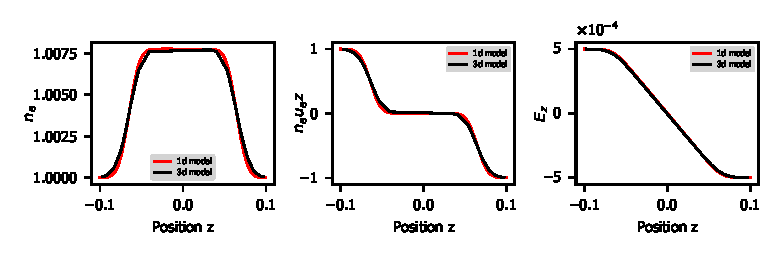
\includegraphics{z_axis_reduction.eps}
    \caption{Comparison of 1D two-fluid model and reduced 1D model on $z$-axis from 3D two-fluid model. The results are both generated on meshes with 64 cells along $z$-axis. No friction term exists. $t = 5 \times 10^{-4}.$}
    \label{fig:z_axis_reduction}
\end{figure}

\todo{Do more thorough tests}

\subsection{A real problem setup}
The problem setting is a cylindrical domain filled with plasma fluids, and with two electrodes on each end, as is sketched in Fig. \ref{fig:sketch_domain}. From the viewpoint of the Euler system, the cylinder is enclosed by a non-penetrating wall whereas the plasma fluids are allowed to inflow and outflow through the electrode surfaces. Regarding the Maxwell system, external electric potentials are applied on the electrodes, and the enclosing boundary is considered insulating. 

Under such a setting, the motions of charged particles of the plasma are driven by the external potential, giving rise to an electromagnetic field, which in turn exerts Lorentz force on the charged particles. This setting is intended for simulating electric arcs.

We discretize the spatial domain by an unstructured mesh doublet ($\mathcal{M}, \Tilde{\mathcal{M}}$) which consists of prisms aligned with the axial direction. The mesh generation is realized by the code developed in \cite{fuchs_2021}. The detailed algorithm is omitted. In principle, a circle is first discretized with a 2D mesh which afterward is extended along the axial direction to form the 3D mesh. Based on the generated primal mesh, a dual mesh conforming to the duality requirements, as is illustrated in Section \ref{sec:mesh_duality}, can be constructed with additional attention on the cut-off boundary that is discussed in Section \ref{sec:boundary_treatment}. An example of the primal and dual meshes is shown in Fig. \ref{fig:primal_dual_meshes}.

\begin{figure}
    \centering
    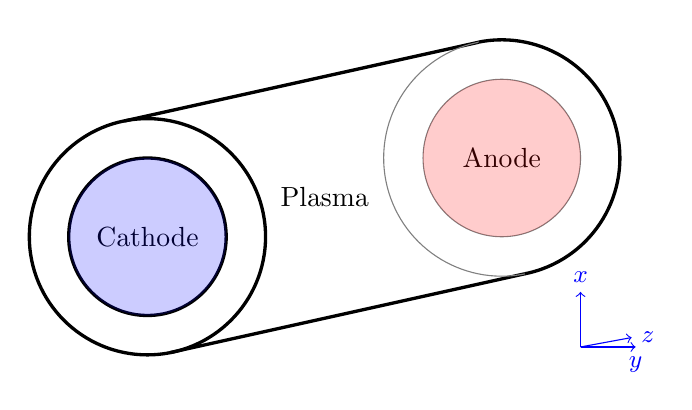
\begin{tikzpicture}
    \coordinate (O1) at (0,0);
    \draw[very thick] (O1) circle (1) node {Cathode};
    \fill[blue, opacity=0.2] (O1) circle (1);
    \draw[very thick] (O1) circle (1.5);
    \coordinate (O2) at (4.5,1) ;
    \draw[gray] (O2) circle (1);
    \node at (O2) {Anode};
    \node at (barycentric cs:O1=1,O2=1) {Plasma}; 
    \fill[red, opacity=0.2] (O2) circle (1);
    \coordinate (S1) at ([shift={(-0.196,0.98)}]O1);
    \coordinate (S2) at ([shift={(-0.196,0.98)}]O2);
    \coordinate (P1) at ([shift={(0.196,-0.98)}]O1);
    \coordinate (P2) at ([shift={(0.196,-0.98)}]O2);
    \coordinate (SS1) at ([shift={({-0.196*1.5},{0.98*1.5})}]O1);
    \coordinate (SS2) at ([shift={({-0.196*1.5},{0.98*1.5})}]O2);
    \coordinate (PP1) at ([shift={({0.196*1.5},{-0.98*1.5})}]O1);
    \coordinate (PP2) at ([shift={({0.196*1.5},{-0.98*1.5})}]O2);
    \draw[very thick] (SS1) -- (SS2);
    \draw[very thick] (PP1) -- (PP2); 
    \draw[gray] (SS2) arc (101.31:180+101.31:1.5);
    \draw[very thick] (PP2) arc (101.31-180:101.31:1.5);
    \begin{scope}[shift={(5.5,-1.4)}]
    \draw[blue, -to] (0,0) -- (0.65,0.12) node[right]{\small $z$};
    \draw[blue, -to] (0,0) -- (0,0.7) node[above]{\small $x$};
    \draw[blue, -to] (0,0) -- (0.7,0) node[below]{\small $y$};
    \end{scope}
    \end{tikzpicture}
    \caption{Sketch of the computational domain: a cylinder filled with plasma and with two electrodes at the ends.\todo{Change the figure}}
    \label{fig:sketch_domain}
\end{figure}

\begin{figure}
    \centering
    %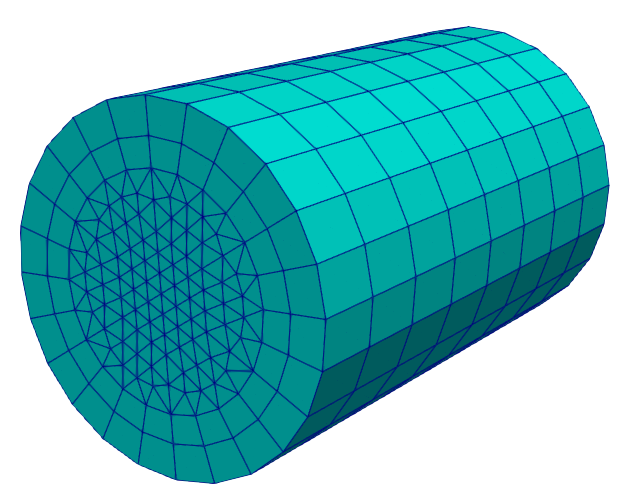
\includegraphics[scale=0.4]{primal_mesh.png}
    \hspace{2cm}
    %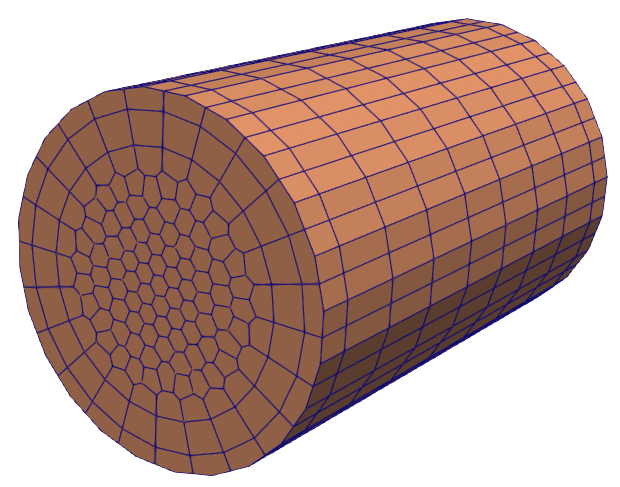
\includegraphics[scale=0.4]{dual_mesh.png}
    \caption{Primal (left) and dual (right) meshes used for the 3D testing case. They are generated by the code developed in \cite{fuchs_2021}.}
    \label{fig:primal_dual_meshes}
\end{figure}

\subsection{Numerical results}
Now comes the point to finally present the numerical results of the AP scheme on the Euler-Maxwell system in a 3D domain. To recap the problem setting and BCs, see Section \ref{sec:problem_description} and \ref{sec:numerical_experiement_bc}. We consider the two-fluid situation where the plasma is composed of electrons and ions. The mass ratio $m_i / m_e$ is equal to $10^4$. The friction term (\ref{equ:collision_rescaled}) is included with $\alpha^\text{coll} = 32$. Other effects like recombination or ionization are not considered yet.  

The initial state is
\begin{equation*}
    n_i(x,y,z,0) = n_e(x,y,z,0) = 1, \ \ \  p_i(x,y,z,0) = p_e(x,y,z,0) = 1.
\end{equation*}
All the other quantities are vanishing initially. The cathode is grounded, and the anode has potential 1.0 throughout the simulation, namely $\varphi^-(t) = 0, \varphi^+(t) = 1.0$. It is intended to see how a stationary system responds to an applied voltage. We would like to remark that such an initial state is conforming to the BCs as well as the quasi-neutral condition $\rho = 0$ so that the quasi-neutrality $\lambda  = 0$ would not incur any initial layer. 

In Fig. \ref{fig:3d_vec_field_E_B_ue} we present the vector fields of the numerical solutions for $\lambda = 1.0, 0.01, 0$ at $t = 0.1$, aiming to give an intuitive visualization. First of all, one \emph{a priori} expects the rotational symmetry in the solutions, which serves as a basic criterion to justify the results. In terms of the 3D structure of the electromagnetic fields, the electric field points from the anode to the cathode, and the magnetic field is spiral-shaped and orthogonal to the electric field. The electrons move in the inverse direction of the electric field. Regarding the asymptotic behavior of the AP scheme, the primary concern is its validity in the limiting case. For this case, the scheme manages to produce a meaningful numerical solution when $\lambda = 0$. Besides, by comparing the solutions for different $\lambda$, the smooth transition from the non-neutrality to quasi-neutrality is observed, which is an implication that the scheme reproduces the asymptotic behavior of the analytical solutions from the non-neutral model to the quasi-neutral one.
\begin{figure}
    \centering
    %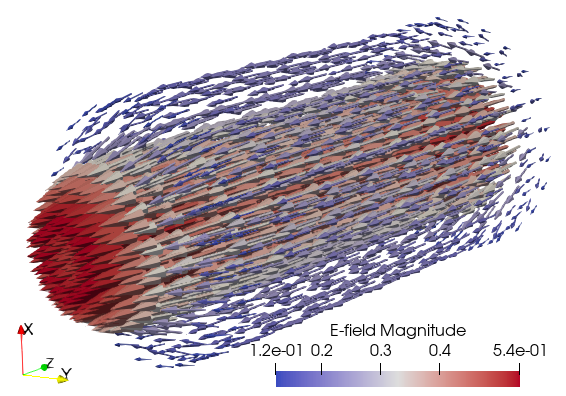
\includegraphics[scale=0.35]{E_lambda_1.png}
    %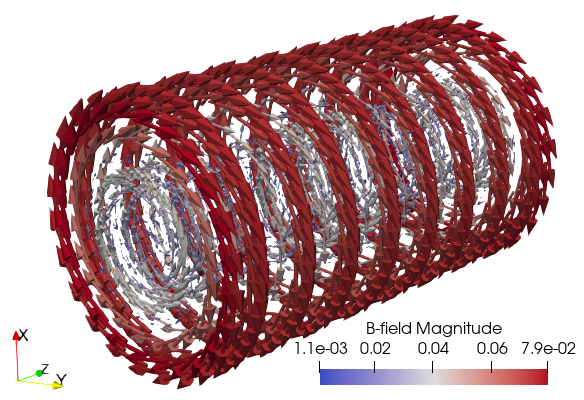
\includegraphics[scale=0.35]{B_lambda_1.png}
    %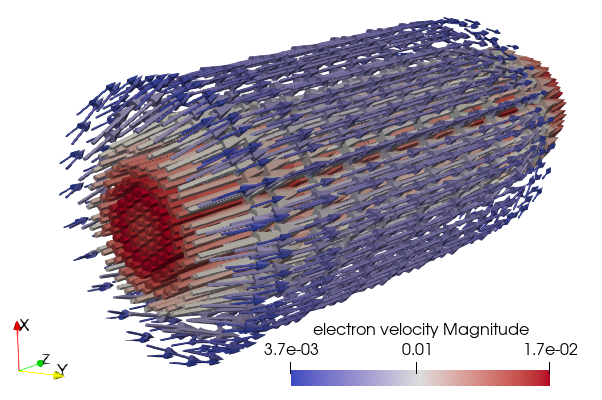
\includegraphics[scale=0.35]{ue_lambda_1.png} \\
    (a) $\lambda = 1.0$ \\
    %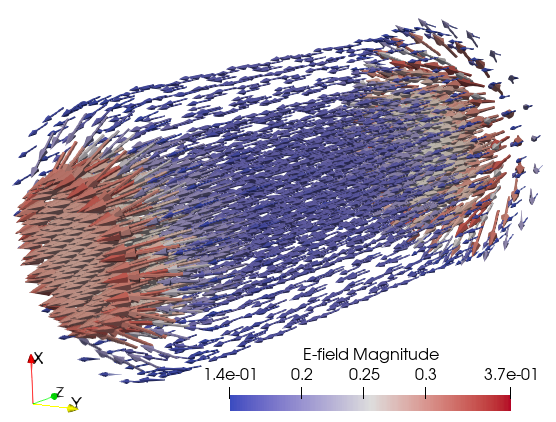
\includegraphics[scale=0.35]{E_lambda_1e-2.png}
    %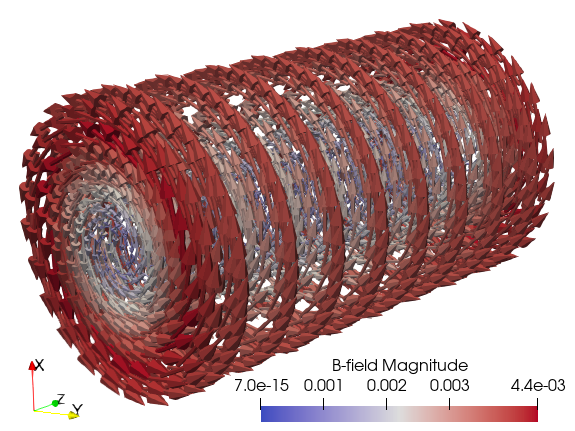
\includegraphics[scale=0.35]{B_lambda_1e-2.png}
    %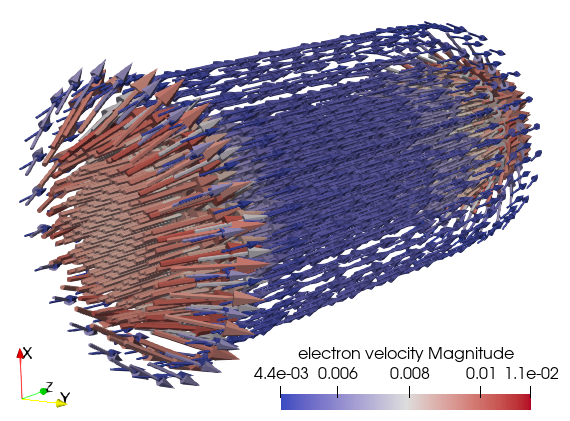
\includegraphics[scale=0.35]{ue_lambda_1e-2.png} \\
    (b) $\lambda = 0.01$ \\
    %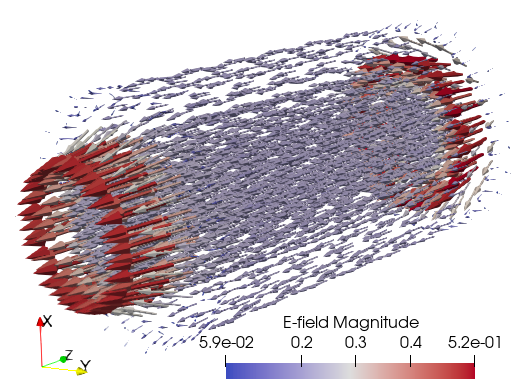
\includegraphics[scale=0.35]{E_lambda_0.png}
    %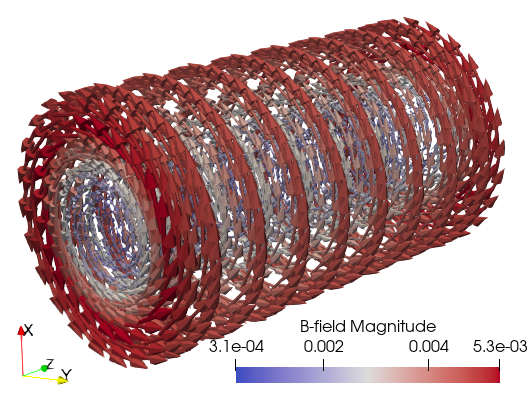
\includegraphics[scale=0.35]{B_lambda_0.png}
    %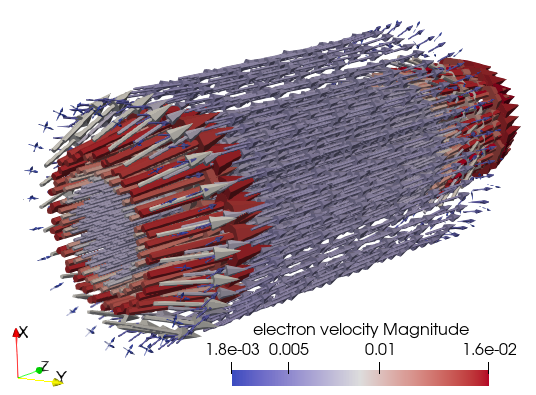
\includegraphics[scale=0.35]{ue_lambda_0.png} \\
    (c) $\lambda = 0$
    \caption{Snapshots of the $\mathbf{E}$-field, $\mathbf{B}$-field, and $\mathbf{u}_e$ for different $\lambda$ at $t = 10$ based on a primal mesh with 1920 cells (8 cells along $z$-axis). } 
    \label{fig:3d_vec_field_E_B_ue}
\end{figure}

We perform the grid study and show the result in Fig. \ref{fig:grid_study_3d}. Meshes with different refinement levels are tested for $\lambda = 1$ and $0.1$ at $t = 1$, and the norms of the quantities are calculated. Due to the high computational cost incurred by the curse of dimensionality, only meshes with limited size are tested and the asymptotic regime of the grid study might be not reached. Nevertheless, it still helps to reveal the independence of solutions with respect to meshes --- the norms of electron density and the magnetic field do not deviate in a divergent manner. The exception of the norm of the electric field possibly results from the singularity caused by the interface of the contacting and insulating surfaces, as will be seen later. 
In Fig. \ref{fig:grid_study_3d_clip_lambda-1e-1} and \ref{fig:grid_study_3d_clip_lambda-0}, we plot the distribution of certain quantities at the cross-section based on different meshes for $\lambda = 0.1$ and $0$ at $t = 1$. Thanks to the rotational symmetry of the problem, the solution at the cross-section suffices to characterize the whole solution. The figures again demonstrate the stability of the numerical solutions with respect to mesh refinement in the sense that qualitatively the same solutions are produced by a series of meshes of different sizes. We would like to point out that singularity arises in the $\mathbf{E}$-field at the interface of contacting and insulating surfaces (two points at the left end and two at the right end). In numerical experiments, we observe an increasing magnitude of the $\mathbf{E}$-field at these points as the mesh is refined. Furthermore, it is noted from Fig. \ref{fig:grid_study_3d_clip_lambda-0} (last two rows) that when $\lambda = 0$, the charges carried by ions and electrons cancel out everywhere as indicated by the quasi-neutral condition $\rho = 0$.

\begin{figure}
    \centering
    %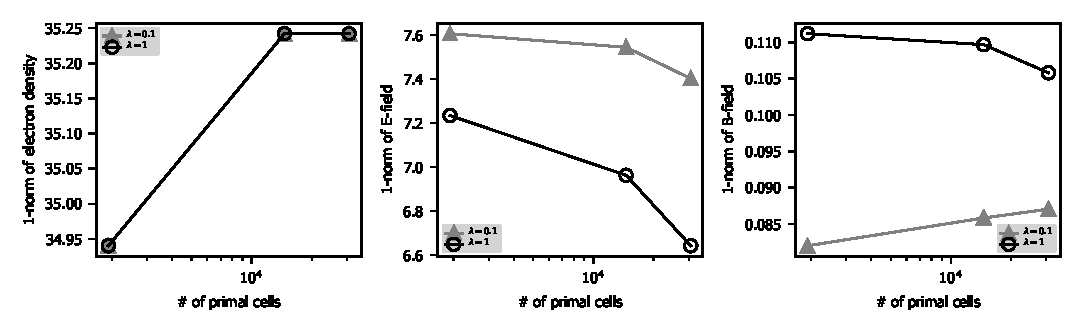
\includegraphics[scale=0.9]{norm_vs_nCell-T_1.eps}
    \caption{1-norms of quantities with respect to different mesh size: The results are computed for $\lambda = 1$ and $0.1$ at $t = 1$.}.
    \label{fig:grid_study_3d}
\end{figure}

\begin{figure}
    \centering
    Refinement 1\hspace{2.5cm}Refinement 2\hspace{2.5cm}Refinement 3\hspace{1cm}
    
    %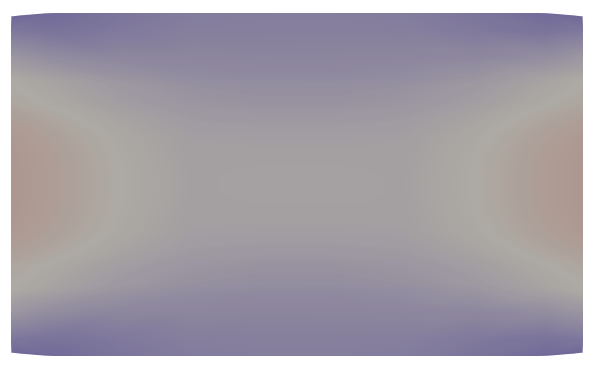
\includegraphics[scale=0.27]{clip_E_T-1_lambda-1e-1_8-2-2.png}
    %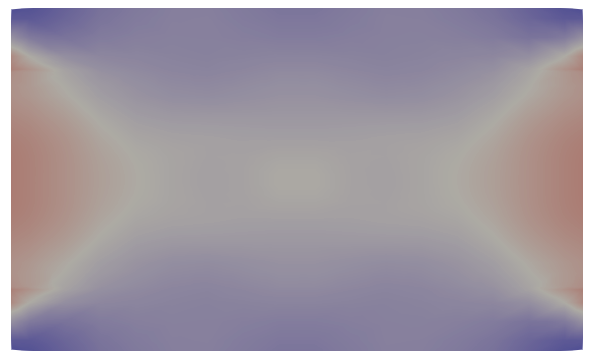
\includegraphics[scale=0.27]{clip_E_T-1_lambda-1e-1_16-3-3.png}
    %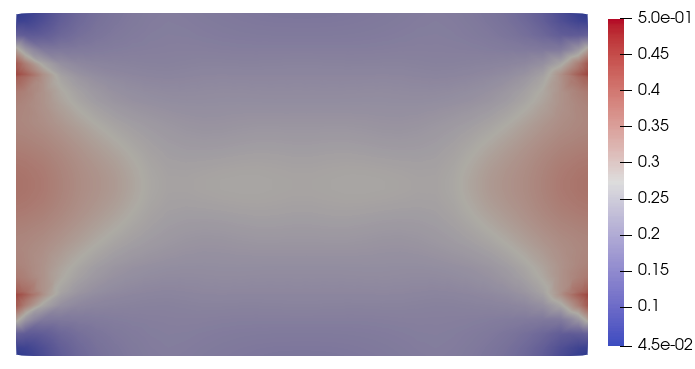
\includegraphics[scale=0.27]{clip_E_T-1_lambda-1e-1_32-3-4.png}
    %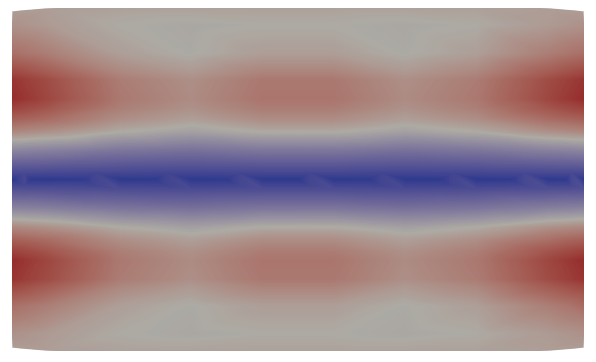
\includegraphics[scale=0.27]{clip_B_T-1_lambda-1e-1_8-2-2.png}
    %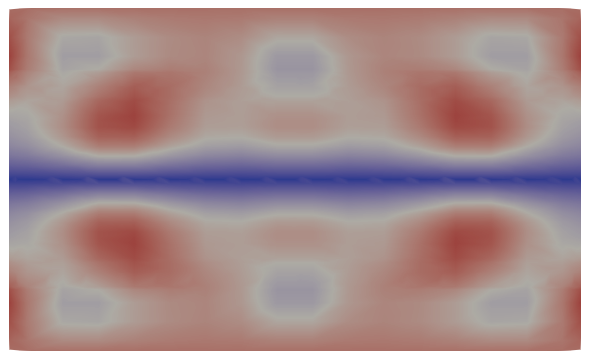
\includegraphics[scale=0.27]{clip_B_T-1_lambda-1e-1_16-3-3.png}
    %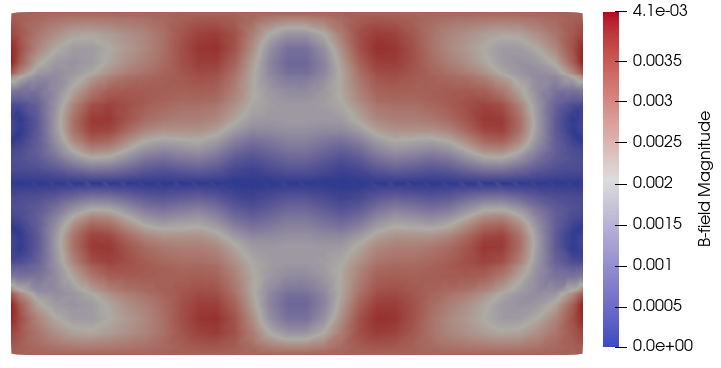
\includegraphics[scale=0.27]{clip_B_T-1_lambda-1e-1_32-3-4.png}
    %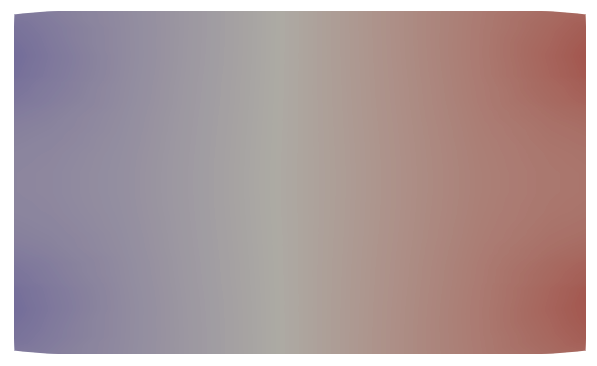
\includegraphics[scale=0.27]{clip_ne_T-1_lambda-1e-1_8-2-2.png}
    %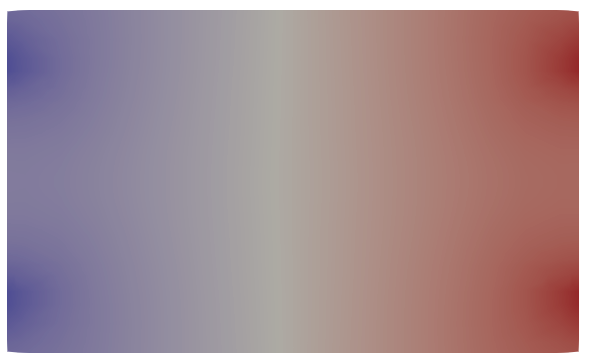
\includegraphics[scale=0.27]{clip_ne_T-1_lambda-1e-1_16-3-3.png}
    %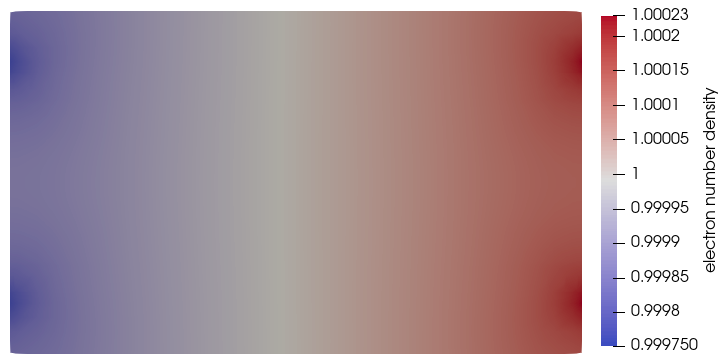
\includegraphics[scale=0.27]{clip_ne_T-1_lambda-1e-1_32-3-4.png}
    %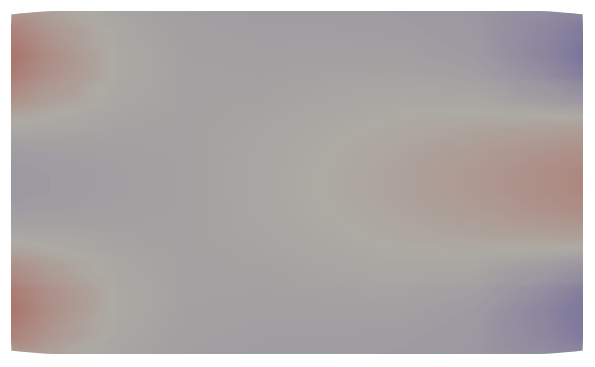
\includegraphics[scale=0.27]{clip_ni_T-1_lambda-1e-1_8-2-2.png}
    %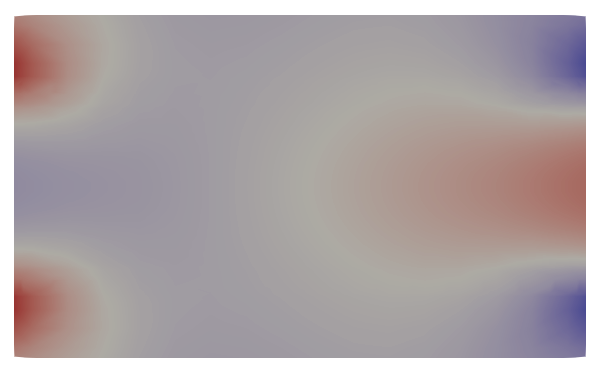
\includegraphics[scale=0.27]{clip_ni_T-1_lambda-1e-1_16-3-3.png}
    %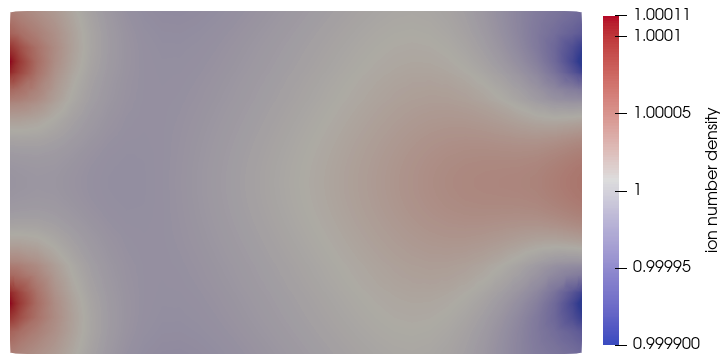
\includegraphics[scale=0.27]{clip_ni_T-1_lambda-1e-1_32-3-4.png}
    \caption{Quantities at the cross-section generated by meshes with different refinement level. Refinement 1: 1920 primal cells; Refinement 2: 14592 primal cells; Refinement 3: 30720 primal cells. The snapshots are computed for $\lambda = 0.1$ at $t = 1$.}
    \label{fig:grid_study_3d_clip_lambda-1e-1}
\end{figure}

\begin{figure}
    \centering
    Refinement 1\hspace{2.5cm}Refinement 2\hspace{2.5cm}Refinement 3\hspace{1cm}
    
    %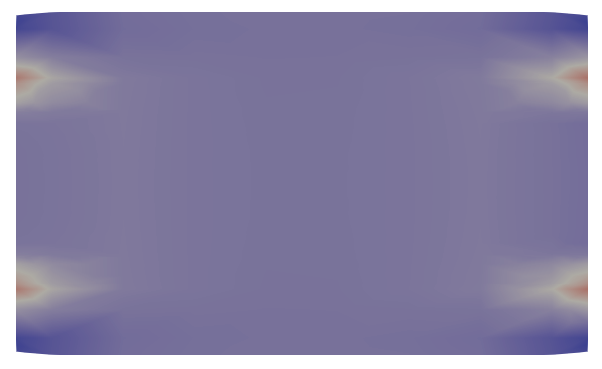
\includegraphics[scale=0.27]{slice_E_T-1_lambda-0_8-2-2.png}
    %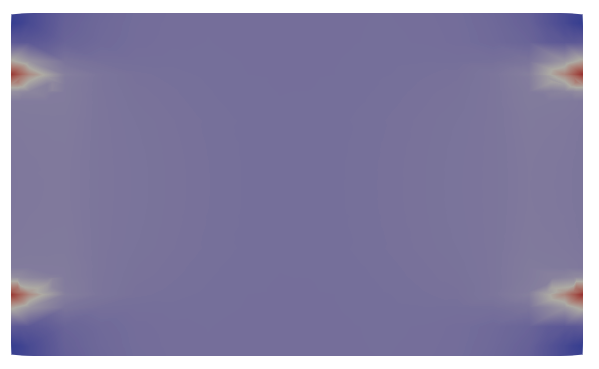
\includegraphics[scale=0.27]{slice_E_T-1_lambda-0_16-3-3.png}
    %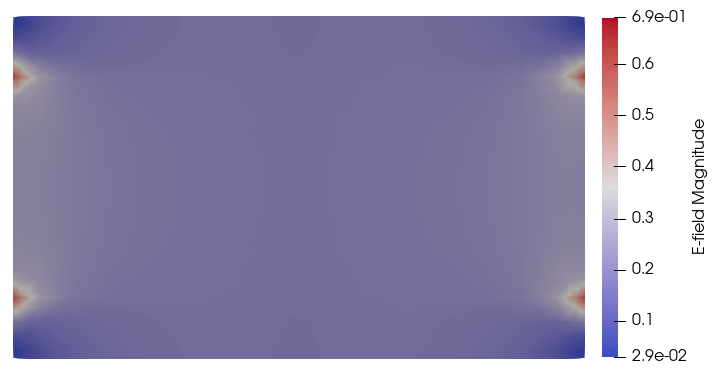
\includegraphics[scale=0.27]{slice_E_T-1_lambda-0_32-3-4.png}
    %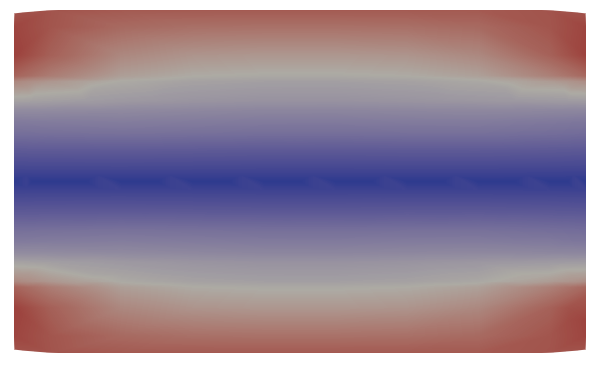
\includegraphics[scale=0.27]{slice_B_T-1_lambda-0_8-2-2.png}
    %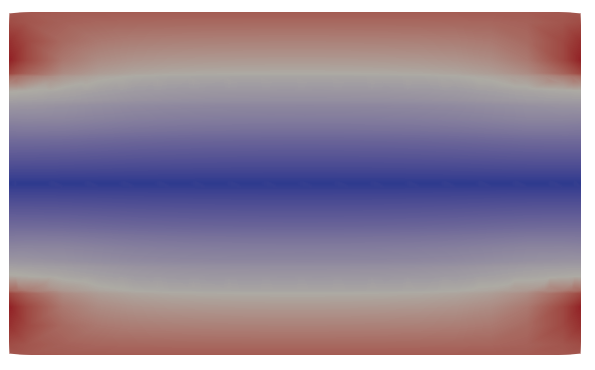
\includegraphics[scale=0.27]{slice_B_T-1_lambda-0_16-3-3.png}
    %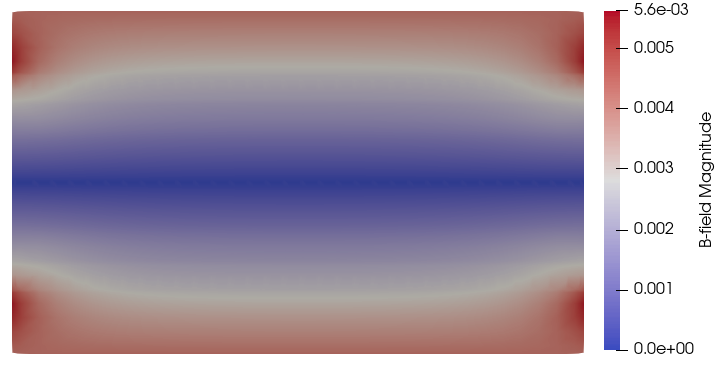
\includegraphics[scale=0.27]{slice_B_T-1_lambda-0_32-3-4.png}
    %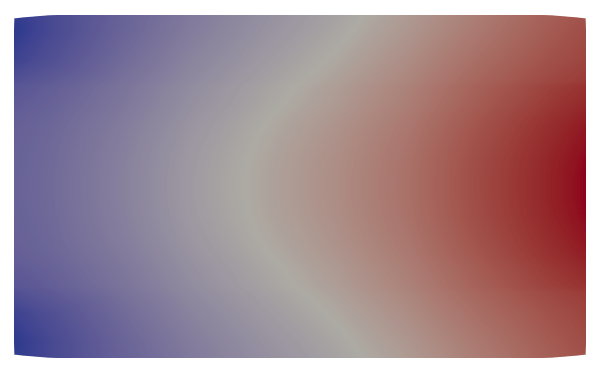
\includegraphics[scale=0.27]{slice_ne_T-1_lambda-0_8-2-2.png}
    %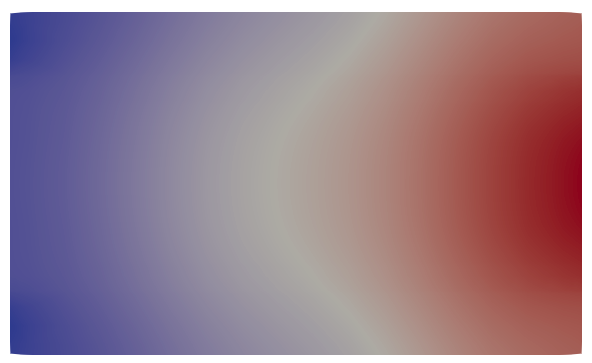
\includegraphics[scale=0.27]{slice_ne_T-1_lambda-0_16-3-3.png}
    %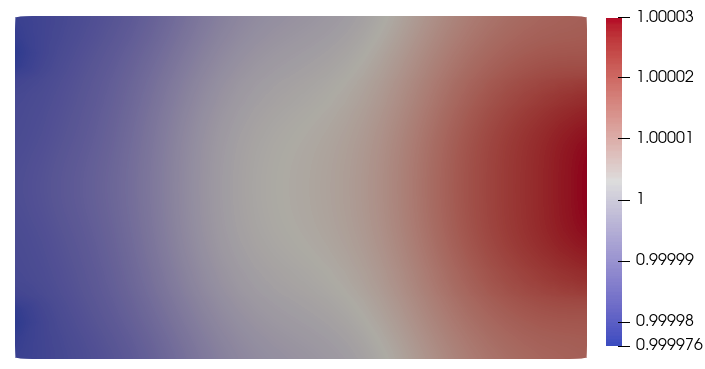
\includegraphics[scale=0.27]{slice_ne_T-1_lambda-0_32-3-4.png}
    %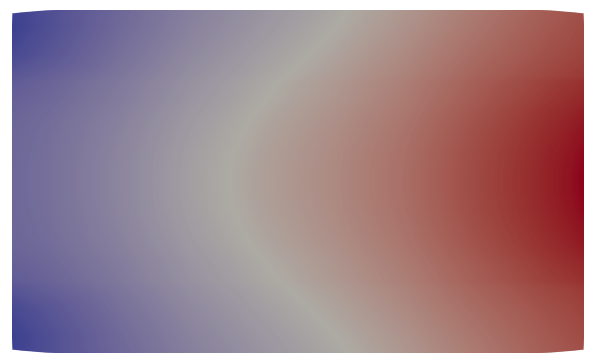
\includegraphics[scale=0.27]{slice_ni_T-1_lambda-0_8-2-2.png}
    %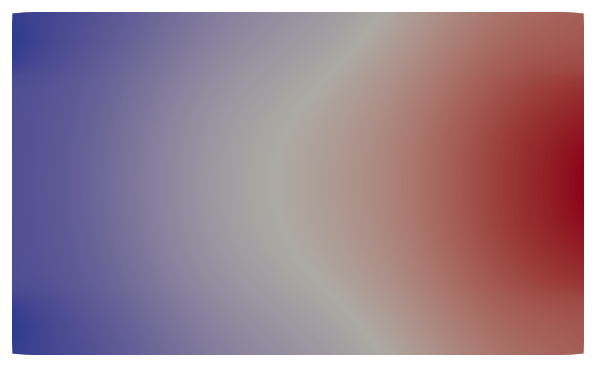
\includegraphics[scale=0.27]{slice_ni_T-1_lambda-0_16-3-3.png}
    %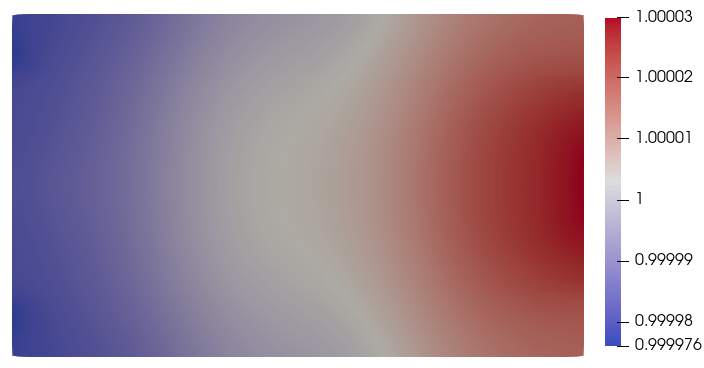
\includegraphics[scale=0.27]{slice_ni_T-1_lambda-0_32-3-4.png}
    \caption{Quantities at the cross-section generated by meshes with different refinement level. Refinement 1: 1920 primal cells; Refinement 2: 14592 primal cells; Refinement 3: 30720 primal cells. The snapshots are computed for $\lambda = 0$ at $t = 1$.}
    \label{fig:grid_study_3d_clip_lambda-0}
\end{figure}

To inspect how the system evolves, we extract the time histories of certain quantities at the origin (the center of the tube) up to $t = 10$ and display them in Fig. \ref{fig:origin-data_vs_time}. Being originally at rest, the system is excited by the suddenly applied voltage and generates oscillations that dampen over time. In general, a large value of $\lambda$ leads to stronger oscillations with larger amplitude whereas smaller $\lambda$ incurs more damping and the system rapidly reaches a steady state. It is a reflection of the shielding effect of plasma which is characterized by the Debye length. It can also be noticed that the electron velocity becomes steady much sooner than ion velocity, which is a consequence of the huge difference in inertia. Besides, the convergence of the discrete model as $\lambda \rightarrow 0$ can be observed---the solution becomes steady over time.
\begin{figure}
    \centering
    %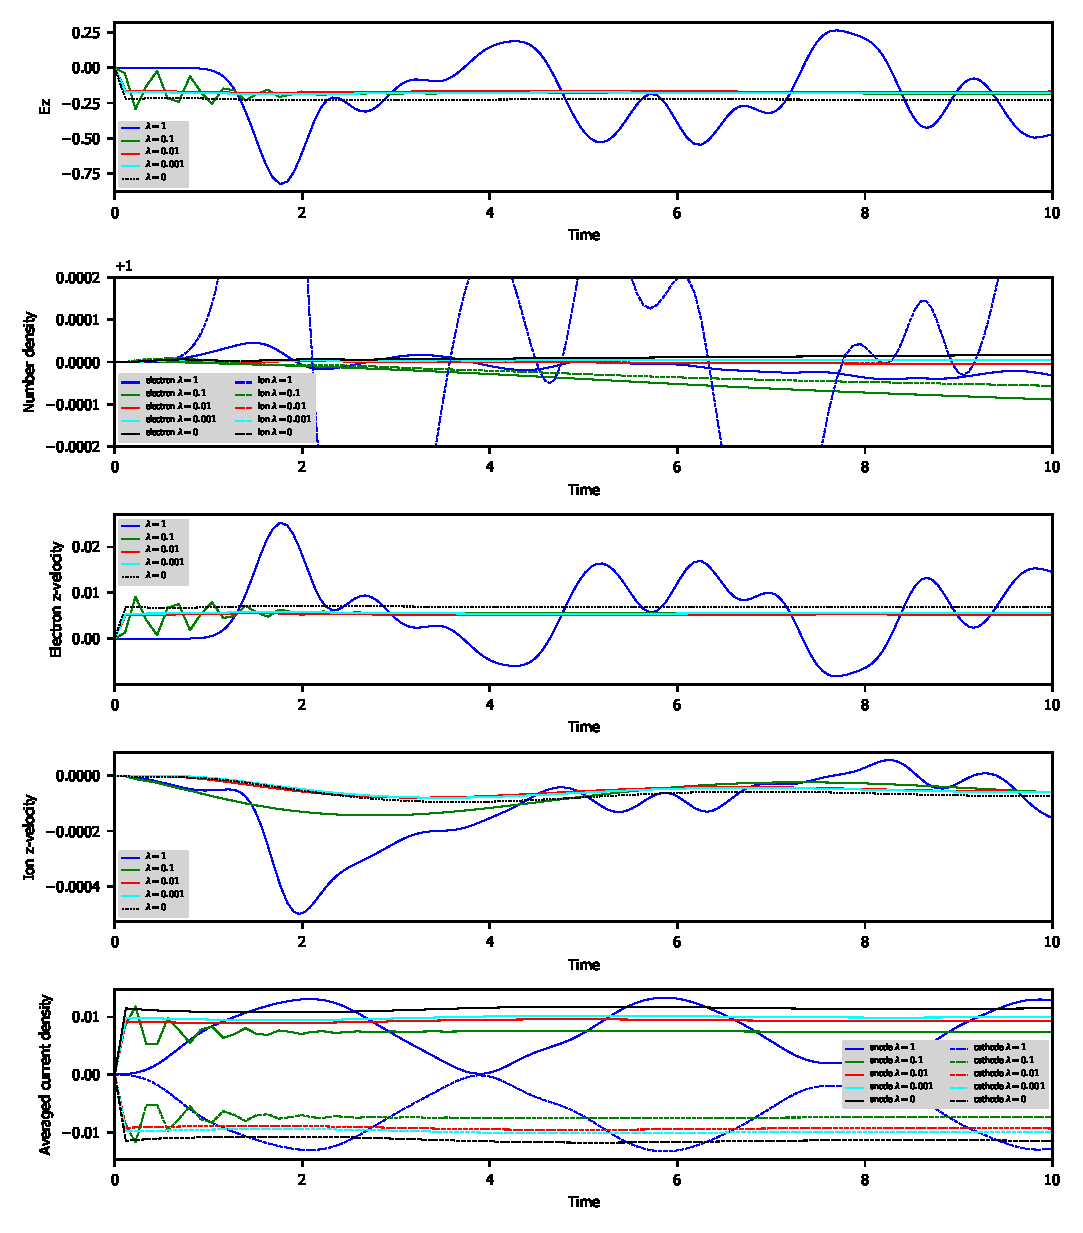
\includegraphics[scale=0.9]{origin-data_vs_time.eps}
    \caption{Time histories of quantities at the origin for different $\lambda$. The simulation is done on a mesh with 1920 primal cells with 8 layers along $z$-axis.}
    \label{fig:origin-data_vs_time}
\end{figure}

A critical sign of quasi-neutrality is the vanishing charge. In fact, in Section \ref{sec:quasi-neutral_limit} we discuss the limiting model where $\rho = 0$ is satisfied. To examine that, the quantities at the $z$-axis over different $\lambda$ are provided in Fig. \ref{fig:zaxis-data_vs_z-T_10}. The right figure demonstrates the approaching and eventual coincidence of electron and ion densities as $\lambda \rightarrow 0$. Furthermore, with relatively small but non-zero $\lambda$, the bulk of the plasma is approximately neutral while the area near the electrodes is not, which is known as a plasma sheath and within such an area the quasi-neutrality is usually inappropriate.
\begin{figure}
    \centering
    %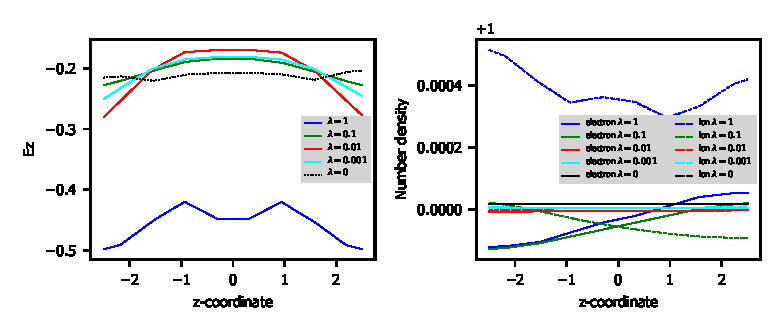
\includegraphics{zaxis-data_vs_z-T_10.eps}
    \caption{Quantities along $z$-axis for different $\lambda$: The results are computed at $t = 10$ on a mesh with 1920 primal cells with 8 layers along $z$-axis.}.
    \label{fig:zaxis-data_vs_z-T_10}
\end{figure}

In Fig. \ref{fig:clip-ne-nue-T_10} the distribution of the electron number density and velocity at the cross-section is displayed. In the non-neutral case, the electrons accumulate near the anode, and the velocity is distributed rather uniformly. With the model approaching quasi-neutrality $\lambda = 0$, the electrons move slower in the bulk area while they are accelerated to high speed at the edge of electrodes, and they tend to accumulate in the middle pass.
\begin{figure}
    \centering
    \begin{subfigure}[b]{0.4\textwidth}
        \centering
        %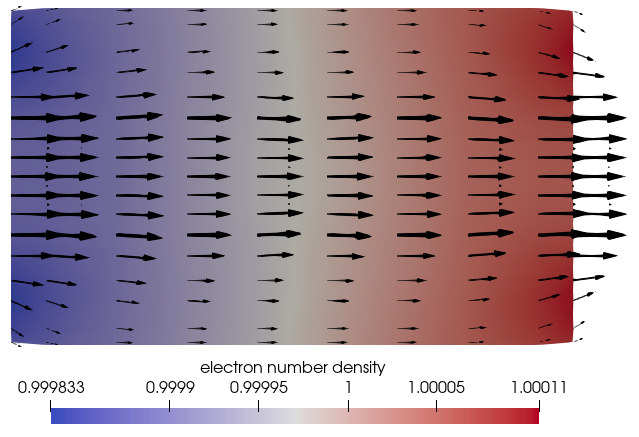
\includegraphics[scale=0.4]{clip-ne-nue-T_10-lambda_1.png}
        \caption{$\lambda = 1$}
    \end{subfigure}
    \begin{subfigure}[b]{0.4\textwidth}
        \centering
        %\includegraphics[scale=0.4]{clip-ne-nue-T_10-lambda_1e-1.png}
        \caption{$\lambda = 0.1$}
    \end{subfigure}
    \begin{subfigure}[b]{0.4\textwidth}
        \centering
        %\includegraphics[scale=0.4]{clip-ne-nue-T_10-lambda_1e-2.png}
        \caption{$\lambda = 0.01$}
    \end{subfigure}
    \hspace{0.2cm}
    \begin{subfigure}[b]{0.4\textwidth}
        \centering
        %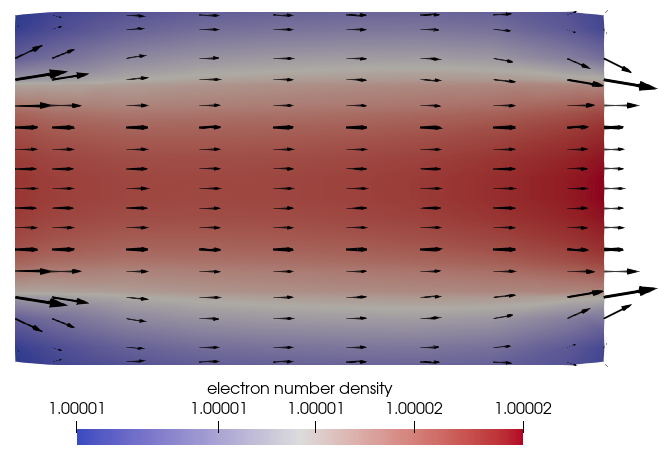
\includegraphics[scale=0.38]{clip-ne-nue-T_10-lambda_0.png}
        \caption{$\lambda = 0$}
    \end{subfigure}
    \caption{Electron number density and velocity vector at the cross-section. The results are computed at $t = 10$ on a mesh with 1920 primal cells with 8 layers along $z$-axis. The velocity vector lengths, which indicates the magnitude, are rescaled by the same factor.}
    \label{fig:clip-ne-nue-T_10}
\end{figure}

\section{Conclusion}
\todo{}



\begin{figure}
    \centering
    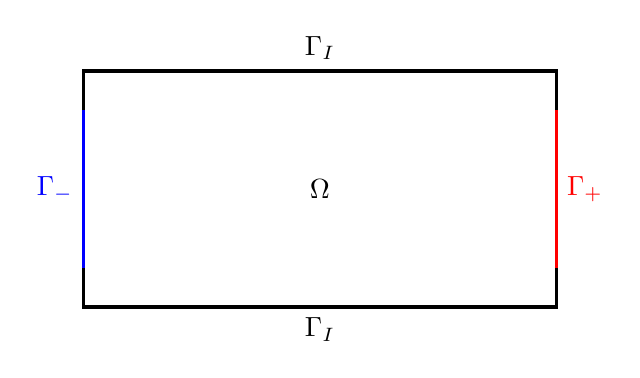
\begin{tikzpicture}
        \coordinate (A1) at (0,1.5);
        \coordinate (A2) at (0,1);
        \coordinate (A3) at (0,-1);
        \coordinate (A4) at (0,-1.5);
        \coordinate (B1) at (6,1.5);
        \coordinate (B2) at (6,1);
        \coordinate (B3) at (6,-1);
        \coordinate (B4) at (6,-1.5);
        \draw[very thick] (A2) -- (A1) -- node[above]{$\Gamma_I$} (B1) -- (B2);
        \draw[very thick] (A3) -- (A4) -- node[below]{$\Gamma_I$} (B4) -- (B3);
        \draw[very thick, blue] (A2) -- node[left]  {$\Gamma_-$}  (A3);
        \draw[very thick, red]  (B2) -- node[right] {$\Gamma_+$}  (B3);
        \node at (3,0) {$\Omega$};
    \end{tikzpicture}
    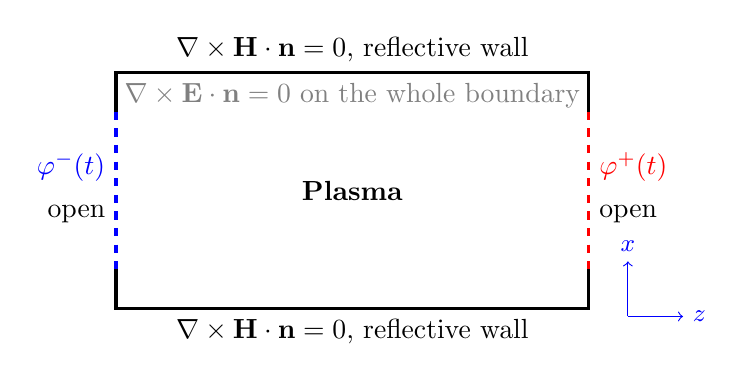
\begin{tikzpicture}
        \coordinate (A1) at (0,1.5);
        \coordinate (A2) at (0,1);
        \coordinate (A3) at (0,-1);
        \coordinate (A4) at (0,-1.5);
        \coordinate (B1) at (6,1.5);
        \coordinate (B2) at (6,1);
        \coordinate (B3) at (6,-1);
        \coordinate (B4) at (6,-1.5);
        \draw[very thick] (A2) -- (A1) -- node[above]{$\nabla \times \mathbf{H}\cdot \mathbf{n} = 0$, reflective wall}  node[below, gray]{$\nabla \times \mathbf{E} \cdot \mathbf{n} = 0$ on the whole boundary} (B1) -- (B2);
        \draw[very thick] (A3) -- (A4) -- node[below]{$\nabla \times \mathbf{H}\cdot \mathbf{n} = 0$, reflective wall} (B4) -- (B3);
        \draw[very thick, dashed, blue] (A2) -- node[left, yshift=0.3cm] {$\varphi^-(t)$} node[left, yshift=-0.3cm] {\textcolor{black}{open}} (A3);
        \draw[very thick, dashed, red]  (B2) -- node[right, yshift=0.3cm]  {$\varphi^+(t)$} node[right, yshift=-0.3cm] {\textcolor{black}{open}}  (B3);
        \node at (3,0) {\textbf{Plasma}};
        \begin{scope}[shift={(6.5,-1.6)}]
        \draw[blue, -to] (0,0) -- (0,0.7) node[above]{\small $x$};
        \draw[blue, -to] (0,0) -- (0.7,0) node[right]{\small $z$};
        \end{scope}
    \end{tikzpicture}
    \caption{Illustration of the boundary conditions: (left) notation of each part of the boundary; (right) boundary conditions at each part of the boundary.\todo{Change the figure}}
    \label{fig:bc}
\end{figure}


\bibliography{ref}
\end{document}